% \documentclass[linenumbers,summarypage,hyperlinks]{outhesis}
\documentclass{outhesis}

% For a bibliography style, you must have the appropriate .bst file
% \bibliographystyle{apj}
\bibliographystyle{prsty}

% Provide the correct margins
\usepackage[top=1in, bottom=1in, left=1.6in, right=1.2in]{geometry}
% If you want a double-sided copy for yourself, uncomment the next line
 % \usepackage[twoside,top=1in, bottom=1in, left=1.6in, right=1.2in]{geometry}

\graphicspath{{/Users/othmane/Documents/Thesis/writing_sample/sample.v0/FIGURES/}}
\usepackage{atlasphysics}
\usepackage{susydefs}
\usepackage{hepparticles}
\usepackage{indentfirst}
\usepackage{subfigure}
\usepackage[makeroom]{cancel}
\usepackage{float}
\usepackage{setspace}

\begin{document}

%% Place Dissertation information here
%% Follow the convention for the use of capital letters 
%% or else the font will not be formatted properly
\author{Othmane Rifki}
\university{UNIVERSITY OF OKLAHOMA}
\college{GRADUATE COLLEGE}
\department{HOMER L. DODGE DEPARTMENT OF PHYSICS AND ASTRONOMY}
\title{Searching for Supersymmetric Particles at the Large Hadron Collider using the ATLAS Detector}
\address{Norman, Oklahoma}
\yr{2016}
\dgname{DOCTOR OF PHILOSOPHY}
%% List your committee members here
\committee{{Dr. Brad Abbott, Chair}, {Dr. S. Lakshmivarahan, Outside Member}, Dr. Mike Strauss, Dr. Chung Kao, Dr. Eric Abraham}

%% Put your dedication here. This is completely optional. Delete it if you don't need it.
%\begin{dedication}
 % 
%\end{dedication}

%% Put your acknowledgements here. This is completely optional. Delete it if you don't need it.
%\begin{acknowledgements}
%  
% \end{acknowledgements}

%% Put your abstract here.

\frontmatter

\maketitle

\mainmatter

%\singlespacing


\section{Overview}
%\label{sec:intro}


As part of our quest to understand and describe the physical world we live in, human beings embarqued on a journey to search for the  most 
fundamental constituents of matter, describe their interactions, and predict their behavior. In short, we want to answer the question 
``what is matter made of?''
The last few decades represented a revolutionary period in the study of fundamental physics.  Several particle accelerators became operational 
and allowed us to disentangle the structure of matter down to a handful of constituents we call elementary particles. The 
most powerful of these accelerators is is the Large Hadron Collider (LHC) at CERN . 
The basic idea of the LHC and other accelerators is to collide particles, 
in our case protons,  at very high energies and take snapshots of these collisions. The goal is to guess the form of the interactions happening 
in each collision and compare the resulting theoretical predictions with the results of our snapshots of the collision, called the experimental data. 
This is one of the strategies that led us to formulate a mathematical framework that describes the elementary particles and their interactions
which is known as the Standard Model of elementary particles (SM). 
When subjected to experimental tests, the SM successfully describes three of the four fundamental forces: electromagnetic, weak, and strong interactions. On the other hand, the SM is not believed to be complete since it fails to explain a number of problems that are still facing today's physics community. First, the SM does not incorporate the fourth fundamental force of gravity. Moreover, It does not provide insight on the nature of the ``invisible'' matter that is holding galaxies together, which constitutes $\sim$ 26\% of the energy density of the universe and is known as \emph{Dark Matter}. In addition, the SM does not account for the different masses and mixing of the 12 leptons
 known as the \emph{flavor problem}, and the predominance of matter over antimatter. In order to solve these problems, searches for physics not accounted for by the SM have been pursued at the LHC. The aim is to conduct 
searches for new states of matter from the experimental data and compare it to theoretical models that predict the existence of these new states of matter.
 The experimental data used in 
our analysis has been collected by the ATLAS detector which is one of the most complex particle detectors ever designed. ATLAS takes snapshots of the 
collisions that are happening 40 million times per second and reconstruct what happened in the collision. We analyze this information to test 
if the theoretical models that we are considering are compatible with our experimental data. One of the theories that predict the existence of 
new states of matter is supersymmetry. Supersymmetry is based on a fundamental symmetry between the elementary particles and the particles that 
mediate their interactions. \\

In the remainder of this document, I present an anlysis of data collected by the ATLAS experiment with the aim of comparing it with theoretical predictions 
based on supersymmetric theories. The level of detail is intended for the professional scientific audience. 


\section{Introduction}
% why study elementary particles
% the sucess of the standard model
% the need for bsm: supersymmetry
% the tool to do it: LHC and ATLAS 
% the challenge

% How did we get here?

Of what is the universe made? A question that has intrigued the human curiosity since the dawn of time. 
Today, we are confident that we do not know the answer to this question but a lot of progress has been made
The overeaching aim was to reduce the diversity of the physicsal phenomena to a compact set of constituents
and a unified set of principles.
% Unification and symmetry
%Yet, attempts to answer it has gone through many iterations in order to find a compact set of principles
%that offers a syntheis of the phenomena we observe in the world around us. 
%would describe the world we observe.
%where it was deemed solved at times 
%and unreachable at others. 
Over two thousands years ago, the ancient Greeks  postulated that all is made of Earth, Air, Fire and Water. 
The idea behind this picture is to give a description of the world we observe based on a compact set of principles 
Obvisoulsy, the ancients got it wrong.
Fastfoward to the end of the 19th century, Mendeleev and others made the astonishing remark that by organizing the 
relative atomic masses of chemical elements in an ascending order, elements with similar chemical properties followed a pattern.
The periodic table of elements was born. 
The predictive power of the periodic table led to the anticipation of new elements and their properties that were later discovered.
However, the table lacked compactness and necessitated a more fundamental underlying structure that could 
connect the different elements. At the turn of the century, several important discoveries established 
the existence of the atom and its constituents. The mass of the atom lies in its nucleus with electrons bound to it via the 
electromagnetic force. The nucleus itself is formed from 
protons and neutrons that are ``glued'' togehter by the strong nuclear force (or strong force).
These elements formed the underlying substructure that explained qualitatively the systematic organization of the periodic table.
Moreover, quantum ideas were applied to the atom offering a quantitative description of the origin of structure in atoms and molecules, 
including the chemical elements and their properties.
The decades that followed refined our understanding of the composition of matter through a series of experimental results.
By studying the collisions of protons and neutrons in the 50's and 60's, we came to uncover a plethora of new particles from the same 
family as the proton and neutron which interacted via the strong force, called \textit{hadrons}.
These particles could not be all elementary
\footnote{Elementary particles refer to  particles that cannot be decomposed into further constituents.}
, a classic replay of the argument that atoms were composite based on Mendeleev's table.
A new layer of structure was unfolded to reveal the existence of \textit{quarks}, elementary 
particles that interact via the strong force and make up all hadrons. 
Another puzzle of the 20th century was the continuous energy spectra in the radioactive $\beta$ decay of nuclei which pointed to the 
existence of neutrinos to remedy the energy conservation law in the decay. This process proceeds via the weak nuclear force 
repsonsible for the radioactivity and nuclear fusion, the process that powers the stars.
It turns out that electrons and neutrinos had other relatives referred to as \textit{leptons}.
Similarly, several other quarks were discovered.%, with the latest top quark discovered in 1995. 
The quarks and leptons are collectively referred as fermions and
share a half integer spin, an intrinsic property of elementary particles.
The strong, weak, and electromagnetic interactions are mediated by 
gluons, $W$ and $Z$ bosons, and photons. These are 
elementary particles with an integer spin, 
collectively called bosons. Apart from gravity, all aspects of daily life can 
be described in terms of these interactions.
%The gravitational force is so weak that it only acts at the macroscopic scale.
The lastest discovery happened in 2012 of a new boson, the Higgs boson, 
that allows the quarks and leptons and the $W$ and $Z$ bosons to 
acquire mass.

%A success story
The physics of elementary particles became the most ambitious and organized attempt to answer the question of what the universe is 
made out of. 
Through a mixture of both theorertical insight and experimental input, we now 
know that everything we see in our daily life is formed from quarks and leptons
that interact via the strong, weak, and electromagnetic forces. 
The forms of these forces are determined from basic princples of 
symmetry and invariance.
As a result, a theoretical framework was constructed to synthesize all these 
developments in a quantitative 
calculational tool that became known as the \textit{Standard Model of particle physics} (SM). 
The only inputs needed by the SM are the interaction strengths of the forces and quark and lepton masses to make 
very accurate predictions about the behavior of elementary particles.
For example, the magnetic moment of the electron calculated in the SM is found to agree with the experimental measurement to nine(?) decimal places.
Over the past 30 years, the SM has been vigorously tested across the strong, weak, and electromagnetic interactions. 
It came out triumphant every time. Yet, we know it is not the complete story. 

% the dark side
In 1933, an observation of the Coma Cluster by Zwicky suggested that the galaxies in the cluster were moving too fast to be explained 
by the luminous matter present. The same observation was repeated when looking at the rotation speeds of individual galaxies which 
suggested a dark component of mass, Dark Matter. 
Several independent measurements established that 
not only dark matter is not made out of baryons but it is more 
abundant. 
For example, anistropies in the cosmic microwave background, a radiation 
left over from the Big Bang, were consistent with 
quantum fluctuations from an inflationary epoch \cite{Hu:2001bc,2009AIPC}. 
These fluctuations encoded details about the density of matter 
in the form of 
cosmological parameters as they travelled through space and time to reach 
our experiments.
The astonishing conclusion was that the universe has nearly five times 
as much dark matter as ordinary matter \cite{Bertone:2004pz}.
The supernovae surveys gave direct evidence for an accelerating universe
 \cite{Perlmutter:1998np},
a view that was cemented by the measurement of cosmological parameters
\cite{Adam:2015rua,Ade:2015xua}
which led to the startling discovery that most of the energy density of 
the Universe is in the 
form of an unkown negative-pressure, called dark energy \cite{Scranton:2003in}.
There is an extensive program of experiments 
which will probe the dark energy.% and is beyond the scope of this work. 
%Instead, we turn to dark matter. 
Astrophysics and cosmology told us about 
the existence of dark matter and measured its density to a remarkable 
precision. Particle physics holds the hope to uncover what dark matter is.
In short, all experimental evidence are consistent with a universe 
constructed of 
\begin{itemize}
\item baryons (everyday matter): $\sim 5\%$ 
\item dark matter: $\sim 20\%$ 
\item dark energy: $\sim 75\%$ 
\item neutrinos, photons: a tiny fraction
\end{itemize}

Today, we are in front of many puzzles related to our view of the universe.
Everything we know of, including all particles present in the standard model, 
constitutes only 5\% of the energy budget of the universe. 
The universe is also predominatly composed of matter as opposed to 
anti-matter even though at the start of the universe, they were in equal 
amounts%, baryon assymetry
. The standard model describes the content of 
everyday matter 
and how it interacts but without telling us why it is that way.
Moreover, the standard model only describes these phenomena 
up to an energy scale of $\mathcal{O}\left(100\right)$ \GeV, weak scale.
Beyond this scale lies the realm of phenomena not described by the standard 
model that extend all the way to the Planck scale of 
$\mathcal{O}\left(10^{19}\right)$ \GeV, the limit where the known laws of 
physics apply. 
There is no mechanism to generate mass for 
neutrinos in the standard model. Last but not least, the standard model 
does not incorporate gravity, the fourth fundamental force.
The SM has many limitations since it is unable to account for observed 
features in the universe. 
Thus, there is a need for a theory beyond the standard model.

One of the most prominent extensions of the standard model, 
that addresses many of the shortcomings mentioned above, is a theory based on 
a new symmetry, called supersymmetry.
This symmetry is between the matter particles, fermions, and particles whose
exchange mediates the forces, bosons. Our current description of the world
treats fermions and bosons differently. Supersymmetry puts forward the idea
that fermions and bosons can be treated in a fully symmetric way. 
In other words,
if we exchange fermions and bosons in the equations of the theory, the 
equations will still look the same. An immediate consequence of the theory
is that every standard model particle will have a ``superpartner''.
As a result, we can design experiments to search for these 
supersymmetric particles. The work presented in this thesis is about the search for supersymmetric particles with a specific signature.
The many benefits of supersymmetry will be discussed but here it is worth 
mentioning two important features of the theory: it addresses the question 
of why there is a huge gap between the Planck scale and the weak scale, 
and it provides a dark matter candidate particle. 

Now that we understand what we are trying to do, it is time to address 
the question of how to do it.
For this endeavour, we require two key elements: accelerators and detectors.
The Large Hadron Collider (LHC) at CERN is the world's most energetic 
particle accelerator producing the highest intensity beam of protons 
travelling at 99.99993\% the speed of light. 

colliding beams of proton beams at a center of mass 
energy of 13 \TeV. When two protons collide, many new paerticles are 
created out of 


Many years of experience from Tevatron collider at Fermilab\cite{tevatron}, 
HERA at DESY\cite{hera}, and LEP\cite{lep} at CERN improved the understanding of the 
complex strong interaction dynamics 


% complex detectors


\section{Signal models}
\label{sec:signal}
\subsection{Models already considered in Run-1}
Final states with two same-sign leptons and multiple jets are sensitive to a variety of new physics scenarios. 
In supersymmetric models in particular, such final states can be produced in the decays of heavy superpartners 
involving massive gauge bosons, sleptons or top quarks. 
We list in this section the different simplified models which we use as benchmarks for the choice of signal regions. 


\begin{figure}[h!]
\centering
\subfigure{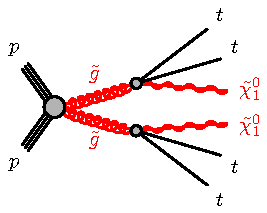
\includegraphics[width=0.24\textwidth]{MODELS/gogo-ttttN1N1}}
\subfigure{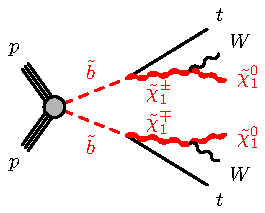
\includegraphics[width=0.24\textwidth]{MODELS/sbsb-ttWWN1N1}}
\caption{Gluino decay via offshell stop (left), and direct sbottom pair production (right).}
\label{fig:feynman_3rdgen}
\end{figure}

\begin{figure}[t]
\centering
\subfigure{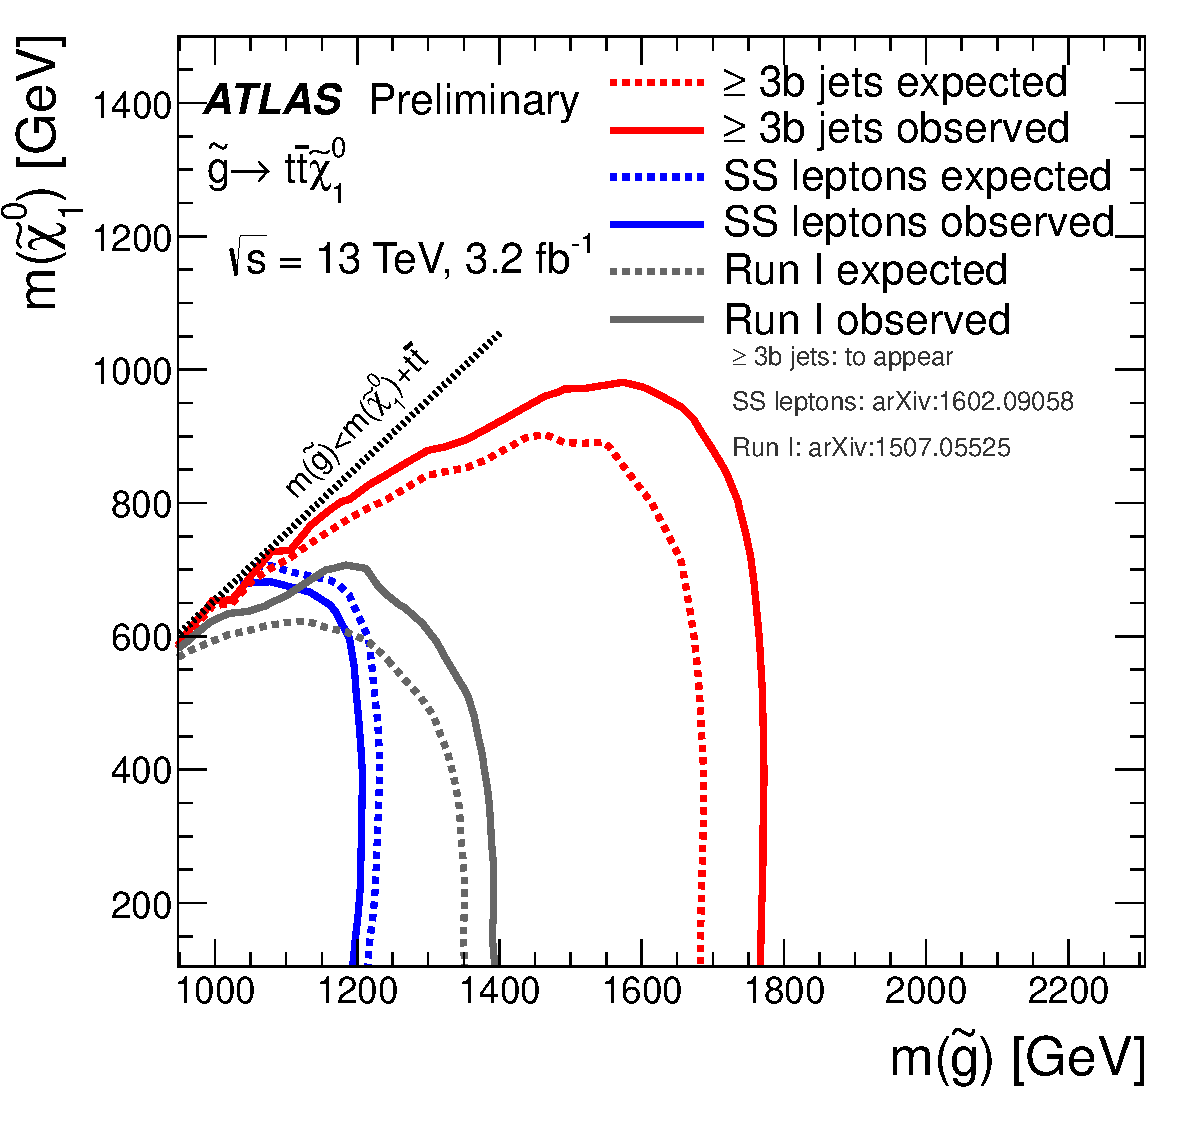
\includegraphics[width=0.49\textwidth]{MODELS/ATLAS_SUSY_Gtt}}
\subfigure{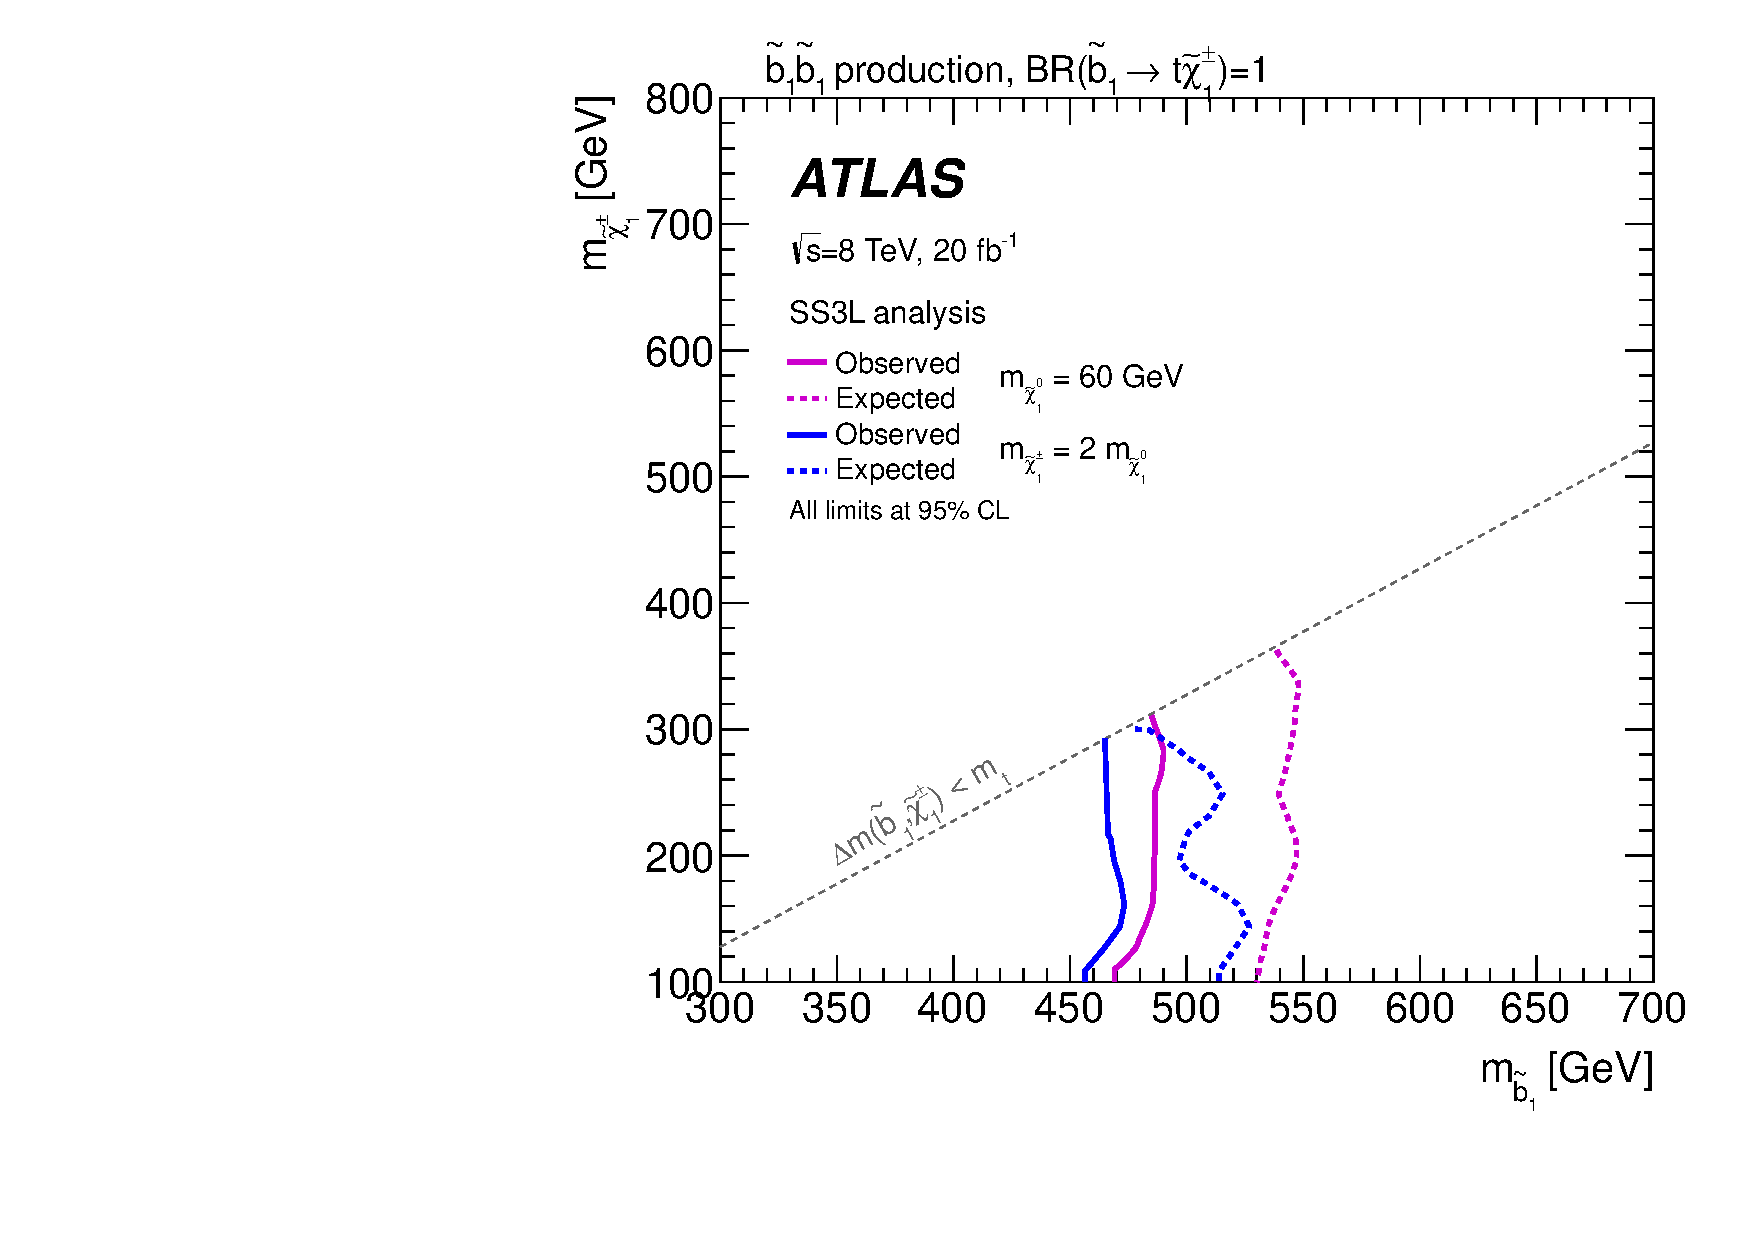
\includegraphics[width=0.49\textwidth]{MODELS/exclusion_sbottom_topC1_both_grids}}
\caption{Exclusion limits on the gluino-stop offshell (left) and direct sbottom (right) scenarios 
set by ATLAS with the 2012 dataset~\cite{DraftSquarkGluinoSummaryPaper}.}
\label{fig:run1excl_3rdgen}
\end{figure}

\par{\bf Gluino-stop offshell $\gluino\to t\bar t\neut$\\}
In this model inspired by naturalness arguments, gluinos are coupling preferentially to stops which are lighter than the other squarks. 
Gluinos are however considered lighter than stops, and decay directly into a $t\bar t\neut$ triplet via a virtual stop (Fig.~\ref{fig:feynman_3rdgen}). 
The pair production of gluinos leads to a final state containing four top quarks and two neutralinos. 
This characteristic final state is accessible through various experimental signatures, which is why this model 
is commonly used as a benchmark to estimate analyses sensitivities. 
The searches performed with run-1 data~\cite{DraftSquarkGluinoSummaryPaper}, 
summarized in Fig.~\ref{fig:run1excl_3rdgen}, showed that the same-sign leptons final state is competitive mainly at large neutralino mass. 
This region of the phase space is consequently given a particular attention in the choice of signal regions described further on. 
In the signal samples referenced in this document, the lightest stop mass is fixed to 10~\TeV and is mostly a $\widetilde{t}_R$ state. 
Only gluino pair production is considered, followed by an exclusive decay in the aforementioned channel. 
\\
\par{\bf Direct sbottom $\sbot\to t\chargino$\\}
In this model, bottom squarks are rather lights and assumed to decay in a top quark and a chargino $\chargino$ (Fig.~\ref{fig:feynman_3rdgen}), 
providing complementarity to the mainstream search which focuses on the channel $\sbot\to b\neut$. 
The final state resulting from the production of a sbottom pair contains pairs of top quarks, of $W$ bosons and of neutralinos. 
While this final state may lead to various experimental signatures, 
the model was considered in run-1~\cite{DraftSquarkGluinoSummaryPaper} 
only by the same-sign leptons and jets search, leading to the exclusion limits presented in Fig.~\ref{fig:run1excl_3rdgen}. 
In the signal samples used by the analysis, the neutralino mass is fixed to 60~\GeV, and the chargino mass to 150~\GeV, while the sbottom mass is varied. 
Only pair production of the lightest sbottom is considered, followed by an exclusive decay in the aforementioned channel. \\


\begin{figure}[h!]
\subfigure{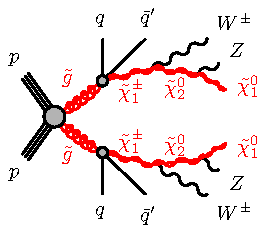
\includegraphics[width=0.24\textwidth]{MODELS/gogo-qqqqWWZZN1N1-C1N2}}
\subfigure{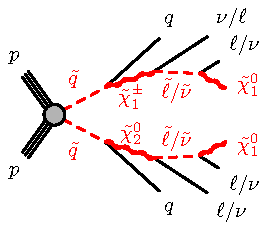
\includegraphics[width=0.24\textwidth]{MODELS/sqsq-qqlllvN1N1-C1N2}}
\subfigure{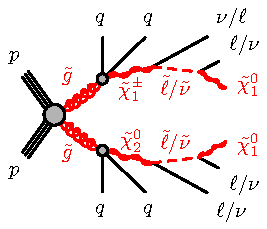
\includegraphics[width=0.24\textwidth]{MODELS/gogo-qqqqlllvN1N1-C1N2}}
\subfigure{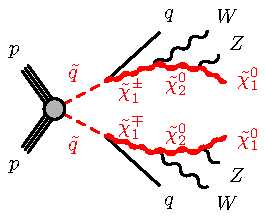
\includegraphics[width=0.24\textwidth]{MODELS/sqsq-qqWWZZN1N1-C1N2}}
\caption{Two-step decays of gluinos and squarks, mediated by gauginos (left) or sleptons (right).}
\label{fig:feynman_1stgen}
\end{figure}

\begin{figure}[t]
\centering
\subfigure{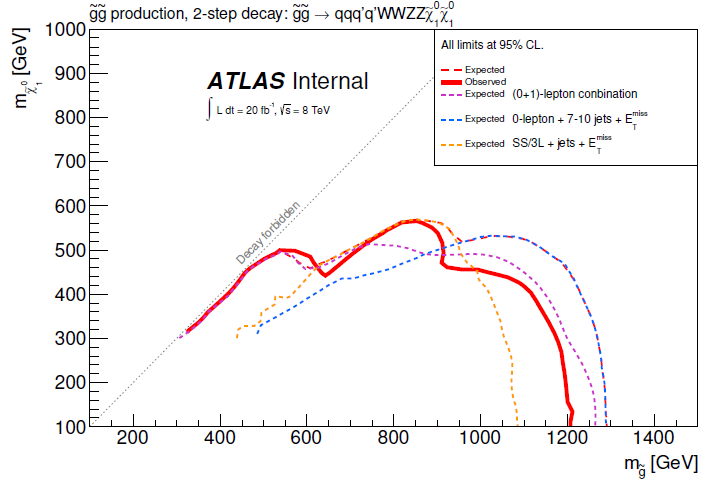
\includegraphics[width=0.49\textwidth]{MODELS/run1excluded_gluino2stepWZ}}
\subfigure{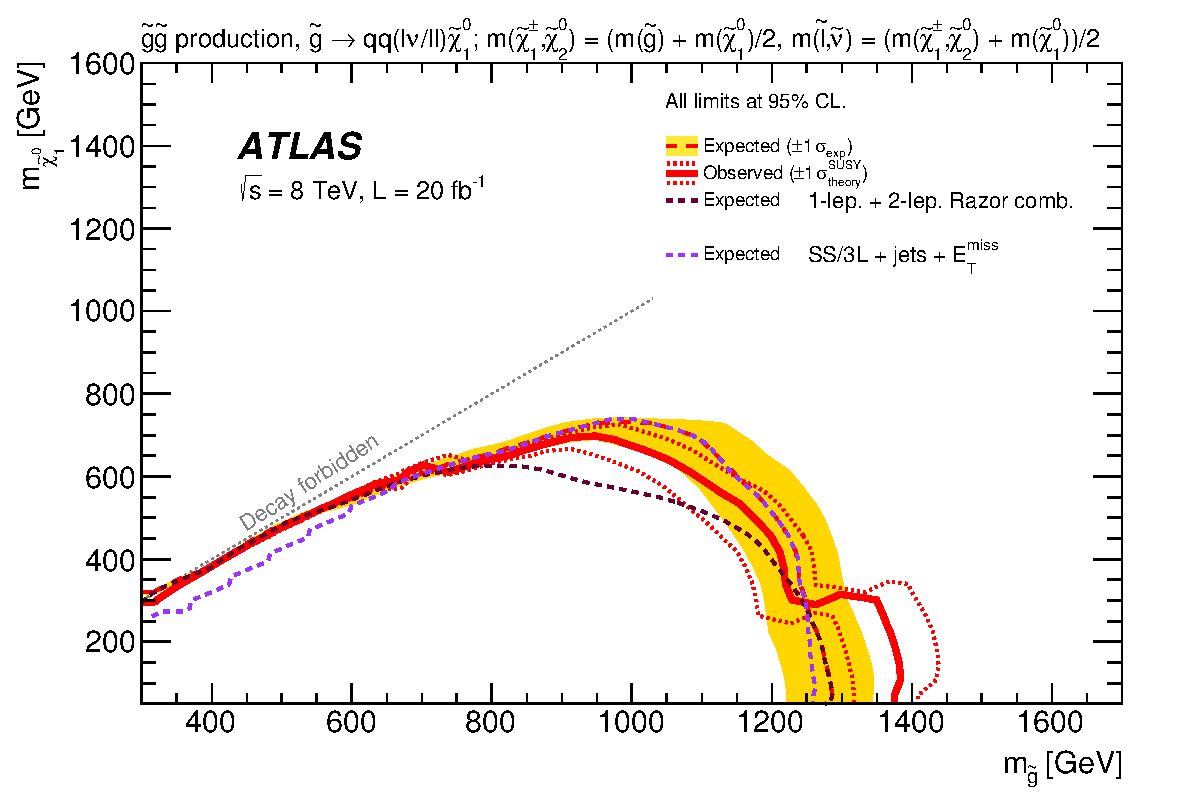
\includegraphics[width=0.49\textwidth]{MODELS/run1excluded_gluino2stepSleptons}}
\subfigure{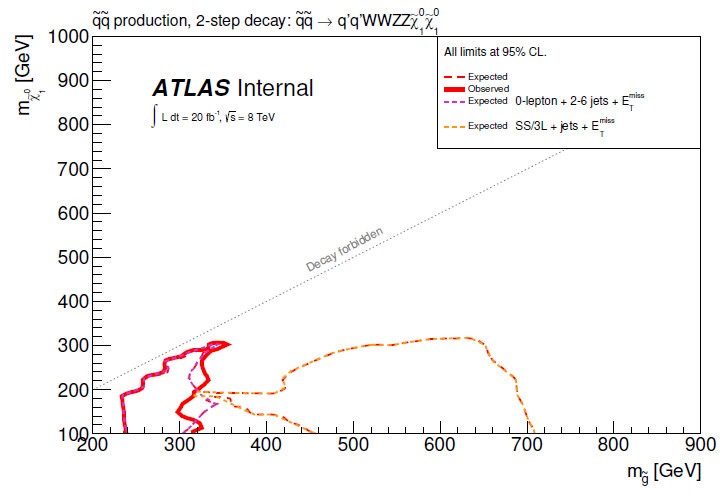
\includegraphics[width=0.49\textwidth]{MODELS/run1excluded_squark2stepWZ}}
\subfigure{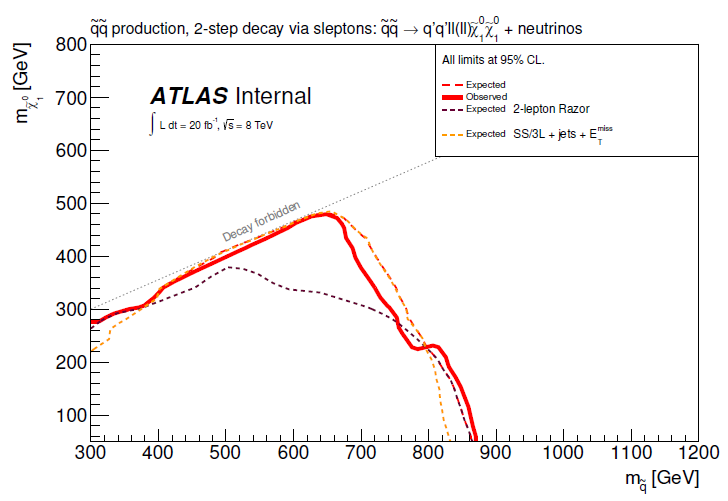
\includegraphics[width=0.49\textwidth]{MODELS/run1excluded_squark2stepSleptons}}
\caption{Exclusion limits on scenarios featuring gluino (top) and squarks (bottom) two-steps decays via gauginos (left) or sleptons (right) 
set by ATLAS with the 2012 dataset~\cite{DraftSquarkGluinoSummaryPaper}.}
\label{fig:run1excluded_1stgen}
\end{figure}

\par{\bf Gluinos and squarks 2-step decays via gauginos\\}
These scenarios feature a less oriented search for gluinos or squarks (save third generation) where gluinos couple preferentially to the latter, 
and squarks decay to charginos (Fig.~\ref{fig:feynman_1stgen} left) with the subsequent cascade $\chargino\to W\tilde{\chi}_{2}^{0} \to WZ\neut$. 
This leads to final states of two light quarks, two $W$ and $Z$ bosons, and two neutralinos 
(with two additional light quarks in the case of gluino pair production). 
Fig.~\ref{fig:run1excluded_1stgen} left shows the exclusion limits obtained with the 2012 dataset~\cite{DraftSquarkGluinoSummaryPaper}; 
in the gluino scenario, the same-sign leptons + jets search provided complementarity at large neutralino mass, 
while its sensitivity in the squark scenario dominated completely. 
In the signal samples used here, the chargino mass is set halfway between the neutralino and squark (or gluino) masses, 
while the neutralino $\tilde{\chi}_{2}^{0}$ mass is set halfway between the chargino and neutralino masses. 
Gluino and squark-antisquark pair production are considered separately in distinct scenarios.  
\\
\par{\bf Gluinos and squarks 2-step decays via sleptons\\}
In these scenarios, gluinos couple preferentially to the squarks of the first two generations, and
the latter decay either to a chargino $\chargino$ or a neutralino $\tilde{\chi}_{2}^{0}$, 
which are assumed to be mass-degenerate, and decay in turn to sleptons (Fig.~\ref{fig:feynman_1stgen} right) 
with $\mathcal{BR}(\chargino\to\nu\tilde\ell) = \mathcal{BR}(\chargino\to\ell\tilde\nu) 
= \mathcal{BR}(\tilde{\chi}_{2}^{0}\to\nu\tilde\nu) = \mathcal{BR}(\tilde{\chi}_{2}^{0}\to\ell\tilde\ell)=50\%$. 
The corresponding final state may contain zero to four charged leptons, neutrinos, two light quarks and two neutralinos 
(with two additional light quarks in the case of gluino pair production). 
Because of the sleptons replacing the gauge bosons featured in the scenarios presented in the previous paragraph, 
these scenarios have comparatively a lower jet multiplicity but a significantly enhanced acceptance in multi-lepton experimental signatures. 
As can be seen on Fig.~\ref{fig:run1excluded_1stgen} right, which presents the exclusion limits obtained with the 2012 dataset~\cite{DraftSquarkGluinoSummaryPaper}, 
the same-sign leptons and jets signature is again very competitive. 
In the signal samples used here, the chargino $\chargino$ and neutralino $\tilde{\chi}_{2}^{0}$ masses are set equal, 
halfway between the neutralino and squark (or gluino) masses, 
while the degenerate sleptons masses are set halfway between these gauginos and the lightest neutralino masses. 
Furthermore, gauginos decay to any slepton flavor with equal probability. 
Gluino and squark-antisquark pair production are considered separately in distinct scenarios. 
\\
\par{\bf Models not considered for the moment\\}
In the publications~\cite{paperSS3L,DraftSquarkGluinoSummaryPaper} of the analysis results obtained with run-1 data, 
exclusion limits were also provided for other signal models, often 
These scenarios included the $\gluino\to tbW\neut$ and $\gluino\to tcW\neut$ simplified models, as well as minimal models featuring 
$R$-parity violation through bilinear terms, gauge-mediated SUSY breaking, or universal extra dimensions. 
These models are not considered here, although interpretations might be proposed for them again in the future. 

\subsection{New models}

%\subsubsection{pMSSM inspired [Sebastien]}

\subsubsection{RPV inspired}
\label{subsec:RPVmodel}

 In supersymmetry, the following superpotential is present :
 \begin{align}
   W = \mu H L + \frac{1}{2} \lambda_{ijk} L_i L_j E_k + \lambda'_{ijk} L_i Q_j D_k + \frac{1}{2} \lambda''_{ijk} U_i D_j D_k
   \label{rpvpotential}
 \end{align}
 where $H$, $L$, $Q$, $E$, $U$ and $D$ are respectively the superpotential associated to the Higgs doublet, the lepton-neutrino doublet, the quark up-down doublet, the right-handed electron, the right-handed up quark and the right-handed down quark.
 The indices $i$, $j$ and $k$ are the flavor indices and $\mu$ , $\lambda_{ijk}$ , $\lambda'_{ijk}$ , $\lambda''_{ijk}$ are the coupling constants.
\\

 The leptonic number violation and the baryonic number violation implied by this potential have an important impact in the physic at low energy
 and do not respect some low energy constraints like the proton decay time limit.
 In $R$-parity conserving (RPC) SUSY models, the $R$-parity is added in order to remove these terms and keep the proton stable.
 However, one can play with the couplings $\mu$ , $\lambda_{ijk}$ , $\lambda'_{ijk}$ and $\lambda''_{ijk}$ in order to violate $R$-parity while respecting the low energy constraints.
 This is called the $R$-parity violation (RPV) SUSY models.
\\

 In this note, we will only consider the case where the coupling constants $\mu$, $\lambda_{ijk}$, $\lambda'_{ijk}$ and $\lambda''_{(i \neq 3) jk}$ are suppressed.
 Therefore, the only non-negligible terms are $\lambda''_{321}TSD$ , $\lambda''_{331}TBD$ and $\lambda''_{323}TSB$ where $T$, $B$, $D$ and $S$ are the superfields associated to the top, bottom, down and strange quark.
 This scenario is predicted by some RPV models like the Minimal Flavor Violation (MFV) scenarios~\cite{Nikolidakis:2007fc,Csaki:2011ge} and leads to the production of same-sign top quarks~\cite{Durieux:2013uqa} (see Fig.~\ref{fig:rpv_diagram}).

\begin{figure}[h!]
\centering
\subfigure{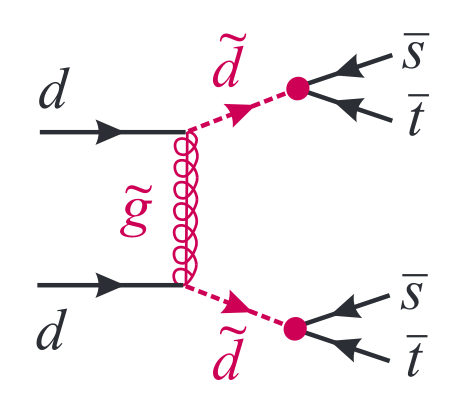
\includegraphics[width=0.24\textwidth]{MODELS/ddfusion.png}}
\subfigure{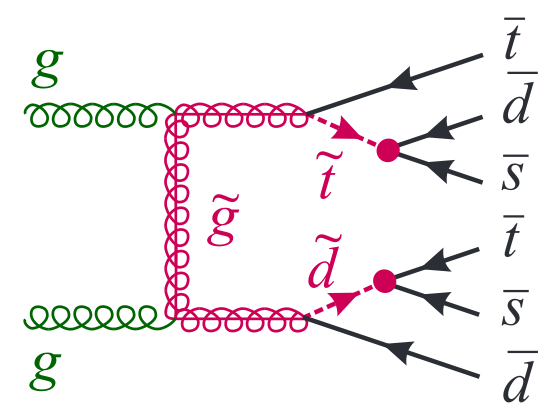
\includegraphics[width=0.27\textwidth]{MODELS/ggfusion.png}}
\caption{Example of diagrams for RPV model for the \textit{d-quark fusion} topology (left), and the \textit{gluon fusion} topology (right) involving the $\lambda''_{321}$ coupling. In both cases, the baryonic number is violated by two units. }
\label{fig:rpv_diagram}
\end{figure}

 In these scenarios, the $R$-parity is not conserved and the LSP is not stable (and therefore cannot be a good dark matter candidate).
 However, the interesting part of this model is that it allows B-violating processes (see Fig.~\ref{fig:rpv_diagram}).
 Actually, the baryonic asymmetry in the universe and the fact that the standard model does not respect this symmetry provides a good motivation for the search for $B$-violation processes at high energy.
 In addition, it was also proved that the violation of the baryonic number by two units involving top quarks could respect the low denergy constraints like the proton decay time limit~\cite{Durieux:2012gj}.
% Therefore, RPV SUSY is good generic model for the search for $B$-violation.
\\

In this analysis, two kind of topologies will be considered:
\begin{itemize}
\item \textbf{d-quark fusion}: Production of two on-shell $d$-squarks with a gluino in $t$-channel and the $d$-squarks decay to an anti-top quark and to one extra jet.
  The squarks will lighter than the gluino and the cross section will mostly depend on the mass of the squark (see Fig.~\ref{fig:rpv_diagram}).
  \begin{align}
    dd \to \tilde{d} \tilde{d}\ ,\ \tilde{d} \to \bar{t}q    
  \end{align}
\item \textbf{gluon fusion}: Production of two on-shell gluinos which decay to a top or an anti-top quark and to two extra jets.
  The gluino will be lighter than the squarks and the cross section will only depend on the mass of the gluino (see Fig.~\ref{fig:rpv_diagram} ).
  \begin{align}
    gg \to \gluino\gluino\ ,\ \gluino \to tqq\ /\ \gluino \to \bar{t}qq'
  \end{align}
\end{itemize}
The extra jets could be either $b$-jet or light jets, depending on the coupling being considered. 
In order to have access to the charge of the top quark, we will only consider the case where the top quark decays leptonically.
At the end, the final states will be composed of two same-sign leptons, at least two $b$-jets, low missing transverse energy (coming from the neutrinos) and extra jets.
\\
% Cross section : soon

 This model was already constrained by ATLAS~\cite{Aad:2014pda} and CMS~\cite{Chatrchyan:2013fea} in Run-1, but those analyses 
 only considered the coupling $\lambda''_{323}$ and the topology of \textit{gluon fusion}.
 A limit of around 900 GeV was found on the mass of the gluino. The full hadronic final state was also exploited in ATLAS~\cite{Aad:2013wta}.



\section{Signal region definition}
\label{sec:sr}
\label{sec:SignalRegDef}

The definitions of the signal regions have been studied to provide an optimal performance for $\sqrt s=13$ TeV collisions and a low integrated luminosity (2-4~\ifb). 
This optimization process was first performed with DC14 MC samples, and was then refined with the more accurate MC15 samples and close-to-final object definitions. 
We chose to categorize the signal regions based on their $b$-jet multiplicity, in continuation of the approach sustained in the Run-1 analysis: 
\begin{itemize}
\item[$\bullet$] Signal region(s) with at least one $b$-jet (``SR1b''): these selections target signal scenarios involving top or bottom quarks, 
mostly related to third-generation squarks, such as the benchmark process $\sbot\sbot^*\to t\bar t\tilde\chi_1^+\tilde\chi_1^-$. 
\item[$\bullet$] Signal region(s) with at least three $b$-jets (``SR3b''): these selections target signal scenarios involving many top or bottom quarks, 
such as the benchmark process $\gluino\gluino\to t\bar tt\bar t\ninoone\ninoone$, 
and with their intrinsically very low background are particularly well suited for scenarios with compressed mass spectra. 
\item[$\bullet$] Signal region(s) with a $b$-jet veto (``SR0b''): these selections allow to increase the sensitivity to signal scenarios without bottom quarks, 
by suppressing most of the top background -- the selections are then dominated by diboson background. 
\end{itemize}
One can notice that there is no dedicated selection for final states with $\ge 2$ $b$-jets: 
it is found to not be particularly useful, as the background is generally dominated by $t\bar t+X$ processes, 
which does not change substantially between $\ge 1$ and $\ge 2$ $b$-jets selections. 
By contrast the difference between $\ge 1$ and $\ge 3$ $b$-jets selections is very important. 

To this first classification we add minimal requirements on the inclusive jet multiplicity: 
\begin{center}
\begin{tabular}{c|c|c|c|c}
Signal region(s) & \multicolumn{2}{c|}{SR0b} & SR1b & SR3b\\\hline
Jets req. & $\ge 3$ ($p_T>50$~GeV) & $\ge 5$ ($p_T>50$~GeV) & $\ge 4$ ($p_T>50$~GeV) & $-$\\
\end{tabular}
\end{center}
As one can see, the SR0b selections were subdivided into two overlapping selections ($\ge 3$ or $\ge 5$ jets, 
also denoted as SR0b5j and SR0b3j) to cover various signal scenarios that lead to differently jet-enriched final states. 
The optimal minimal number of jets and the jet $p_T$ thresholds were defined as part of the DC14-based optimization, through a (\meff, \met, \#jets, jet $p_T$) scan similar to the one described below 
and focused on the few benchmark signal scenarios that were produced for DC14 studies. Only the $\pt$ threshold for SR0b3j was raised from 40 to 50~GeV for homogenization among the SRs since this change had very small impact in the sensitivity.

All these selections are inclusive in terms of leptons (``at least two same-sign leptons''), 
it was found that for these early results no substantial gain would be achieved by considering trilepton final states separately (as was done in the Run-1 analysis) except for SR0b3j, where a $\geq$3 lepton requirement was found to improve the sensitivity to slepton-mediated signals ($\gluino\to q\bar{q}(\ell\ell/\ell\nu)\ninoone$).

To complete the definition of the signal regions, we added requirements on the effective mass \meff{} and missing transverse momentum \met. 
We rely only on these two discriminant variables, well suited for generic SUSY searches, 
as one of the analysis strengths is to be sensitive to a broad range of BSM scenarios and we do not want to overtune it to a restricted set of benchmarks. 

\subsection{Optimization procedure and results}

The optimization of the signal region definitions was carried on with the MC15 samples. % (resp. the 50/25 ns configuration for background/signal). 
We scanned the $(\meff,\met)$ plane for the four selections detailed above, 
looking at the impact of the cuts on various signal benchmarks. 
We used as figure of merit the signal discovery significance (Zn), calculated with {\tt RooStats::NumberCountingUtils::BinominalObsZ} 
assuming an overall $40\%$ systematic uncertainty on the background prediction (as a compromise to the 50\% expected uncertainty on the fake-lepton background and 30\% on the prompt-lepton background). 
We discarded the cut configurations where the background projection was too imprecise, due to limited MC statistics; 
more precisely when the statistical error on the projected background exceeded $30\%$. 
We also focused on signal benchmarks that would provide at least 2 signal events for the considered luminosity. 

Figure~\ref{fig:OptimScan} shows as an example the $(\meff, \met)$ planes for two different signal regions and models.
The resulting maximum discovery significance across the signal grids and the corresponding $(\meff,\met)$ configurations 
are shown in Figure~\ref{fig:OptimSig1} for SR1b, SR3b and SR0b5j. As shown, with 2~\ifb\ of data we can have sensitivity beyond the existing Run-1 limits in some of the models. Note that the Run-1 limits shown in the figures correspond to the best ATLAS limit, not necessarily obtained by the SS/3L analysis.

\begin{figure}[!htb]
\centering
  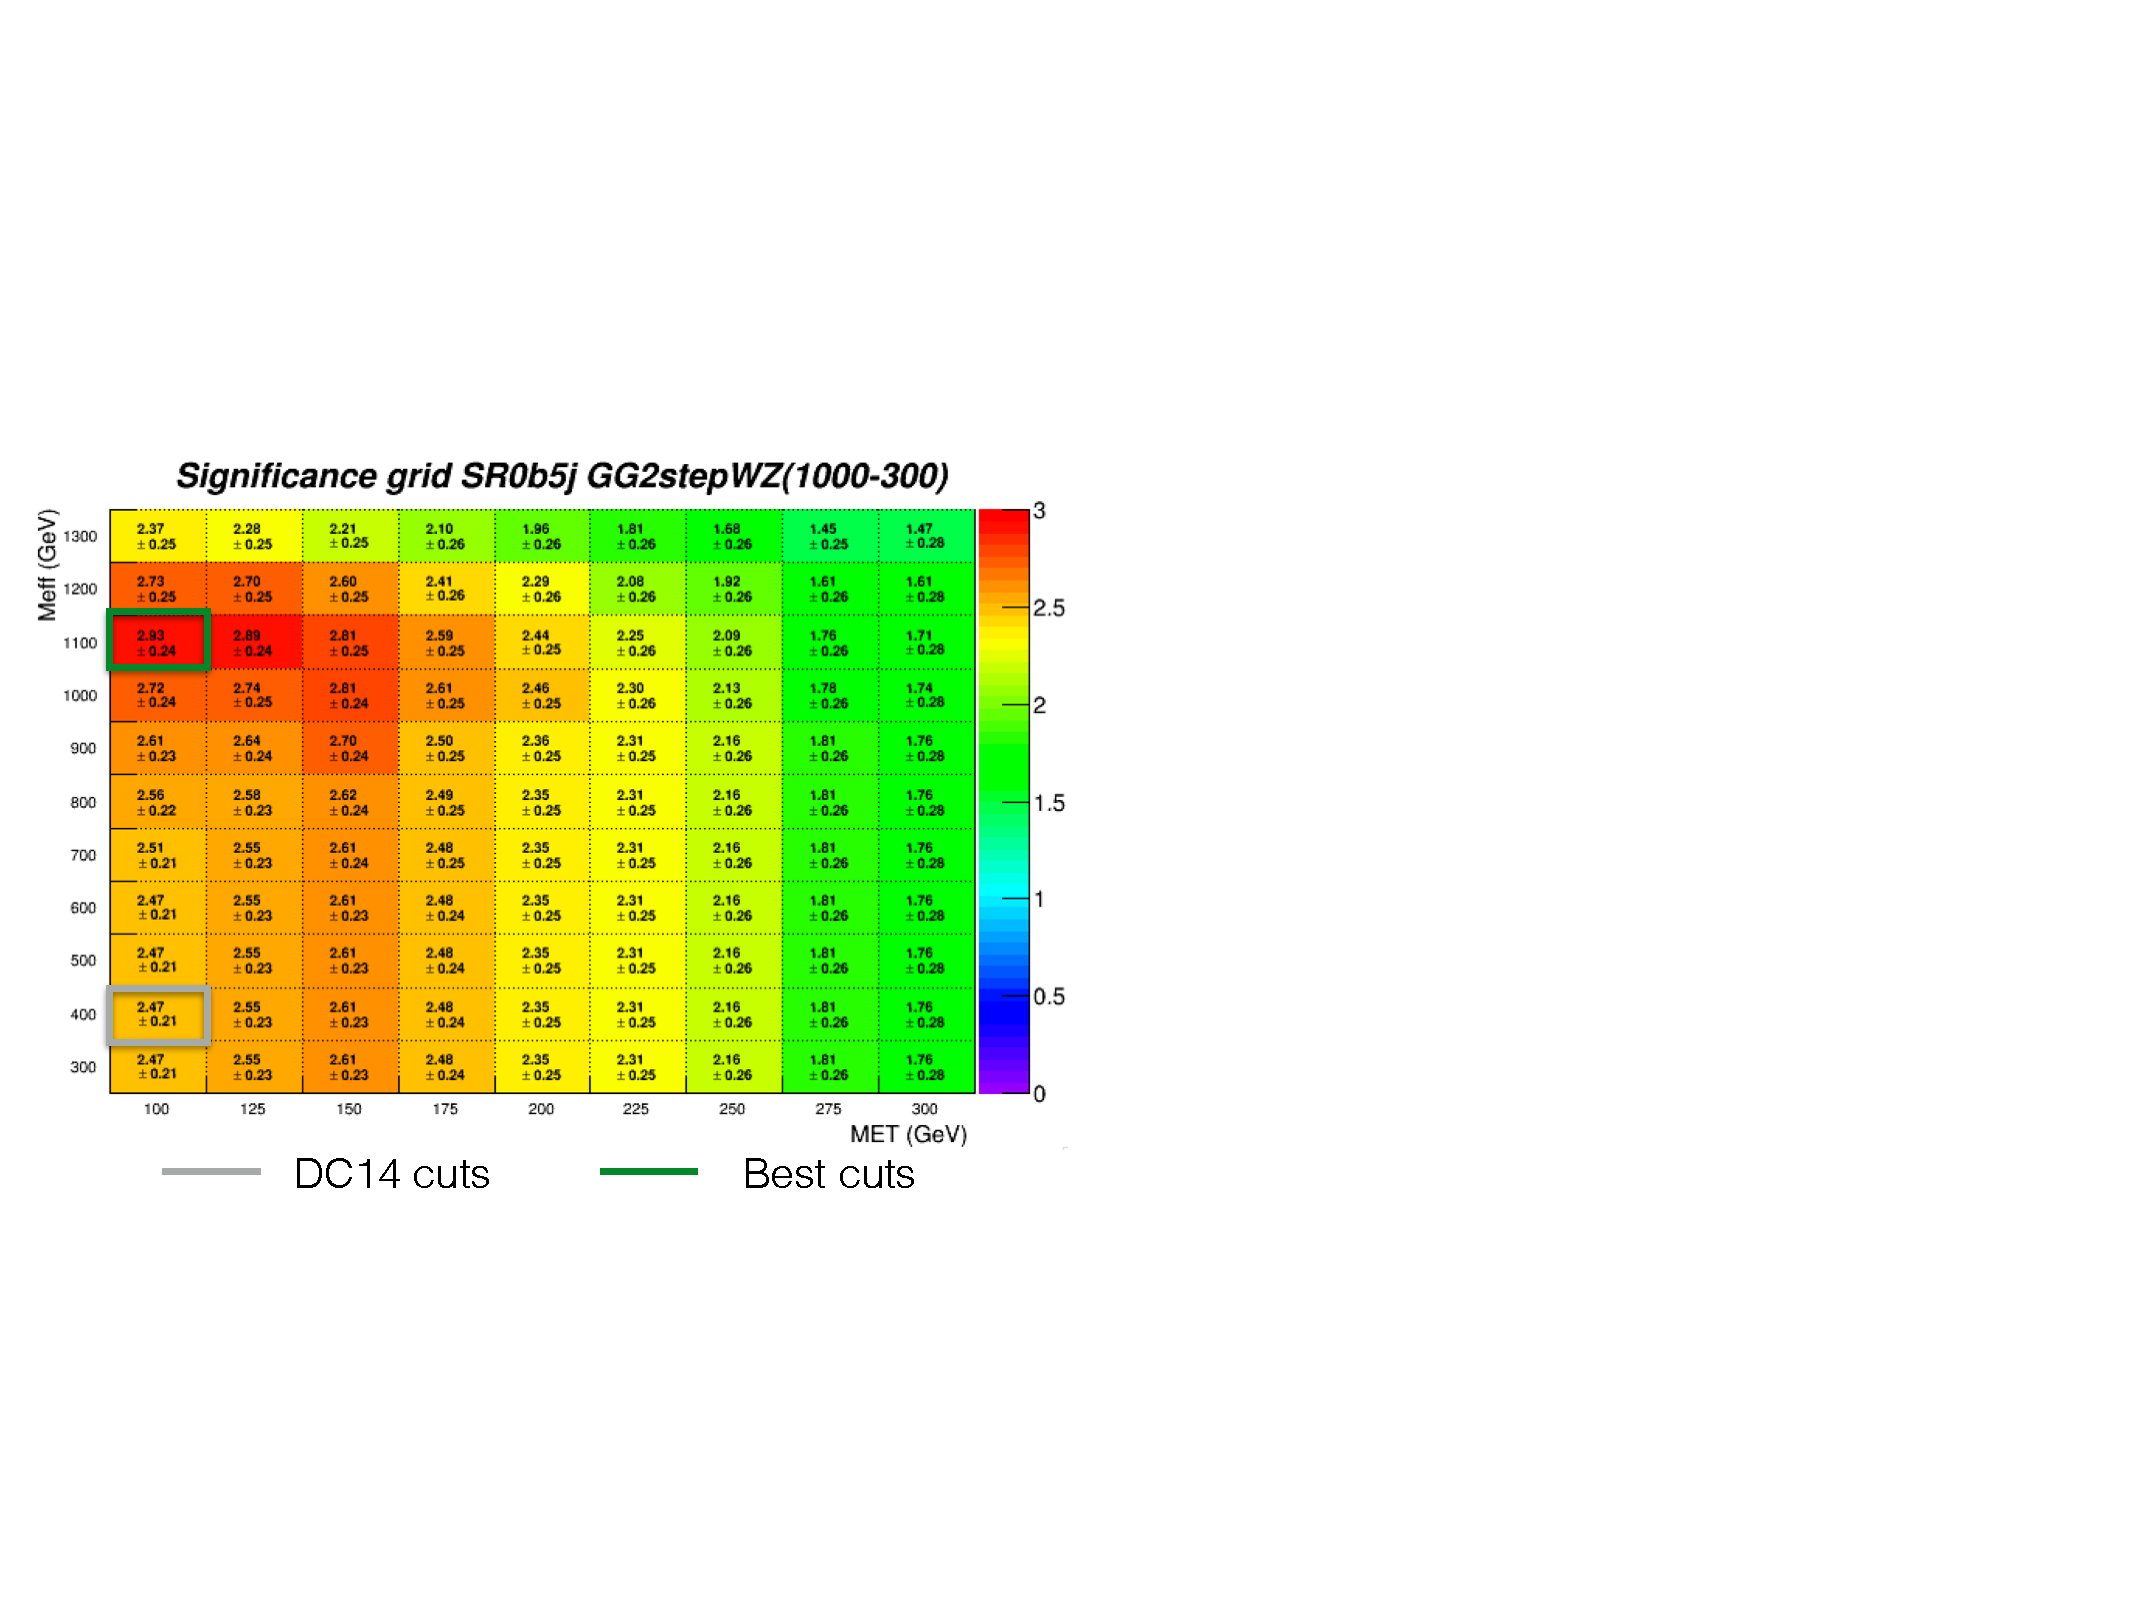
\includegraphics[width=0.49\textwidth]{OPTIMIZATION/Scan1.pdf}
  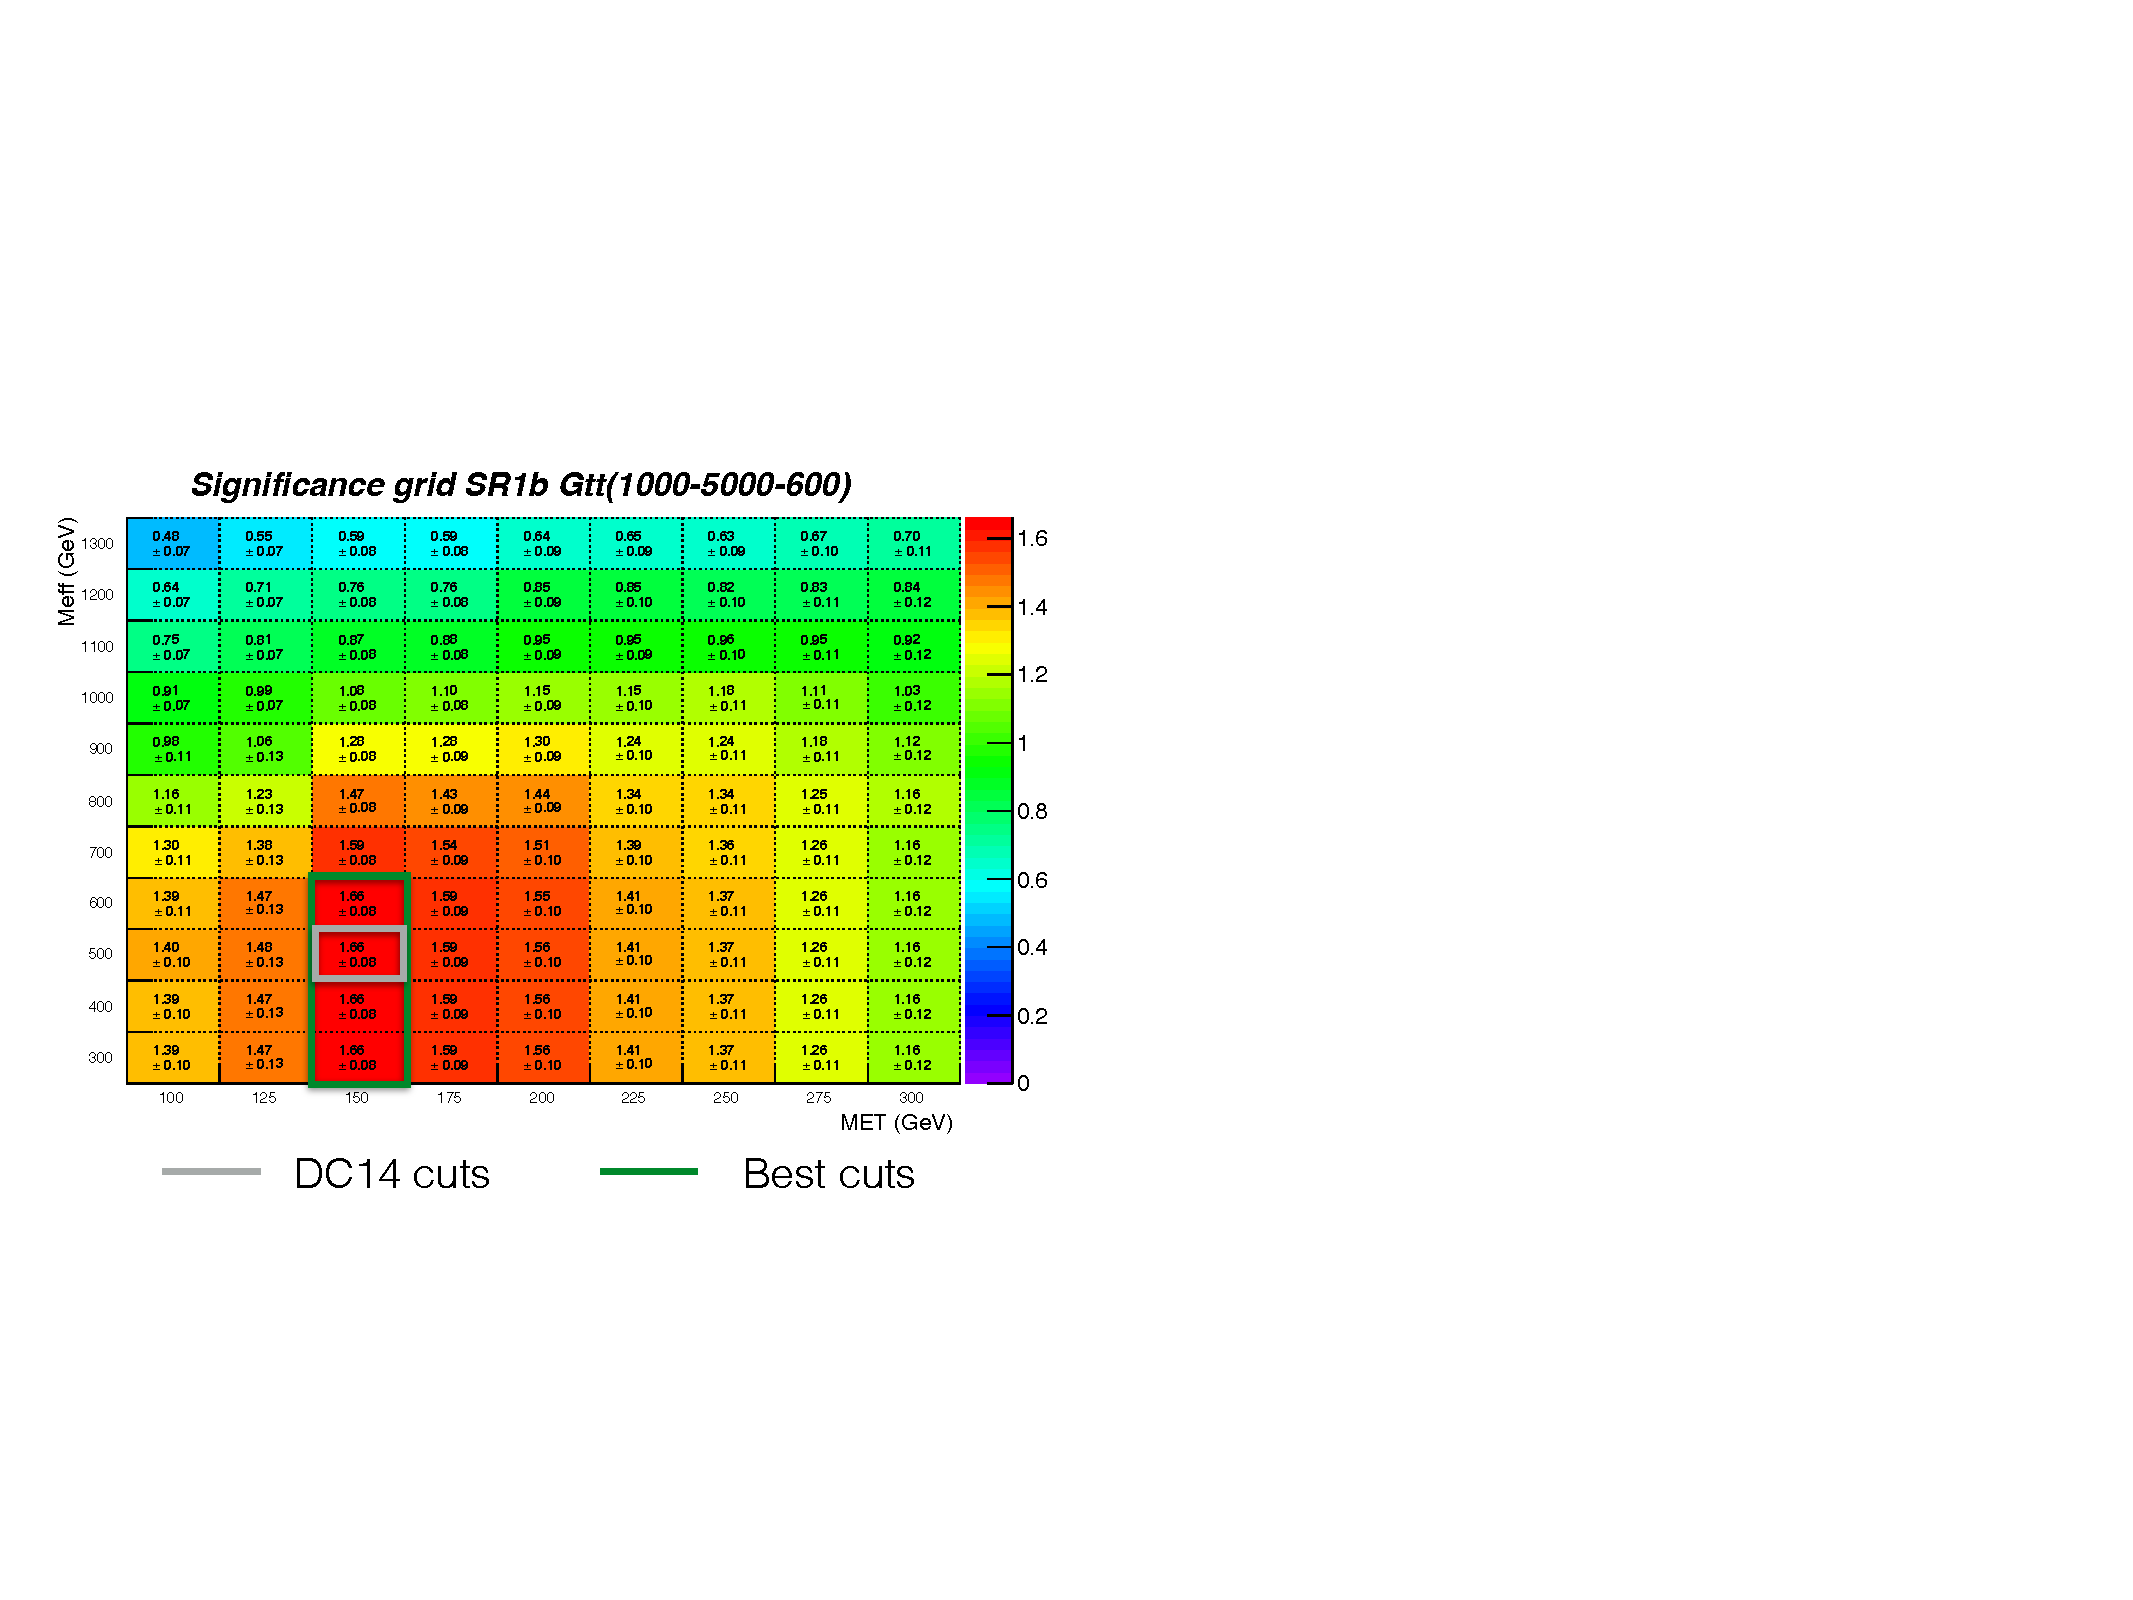
\includegraphics[width=0.49\textwidth]{OPTIMIZATION/Scan2.pdf}
  \caption{Example of (\met, \meff) scans for SR0b5j (left) and SR3b (right). The configurations with maximum significance are highlighted as well as the outcome of the DC14 optimization studies.}
\label{fig:OptimScan}


\end{figure}


%\begin{figure}[!htb]
%\centering
%  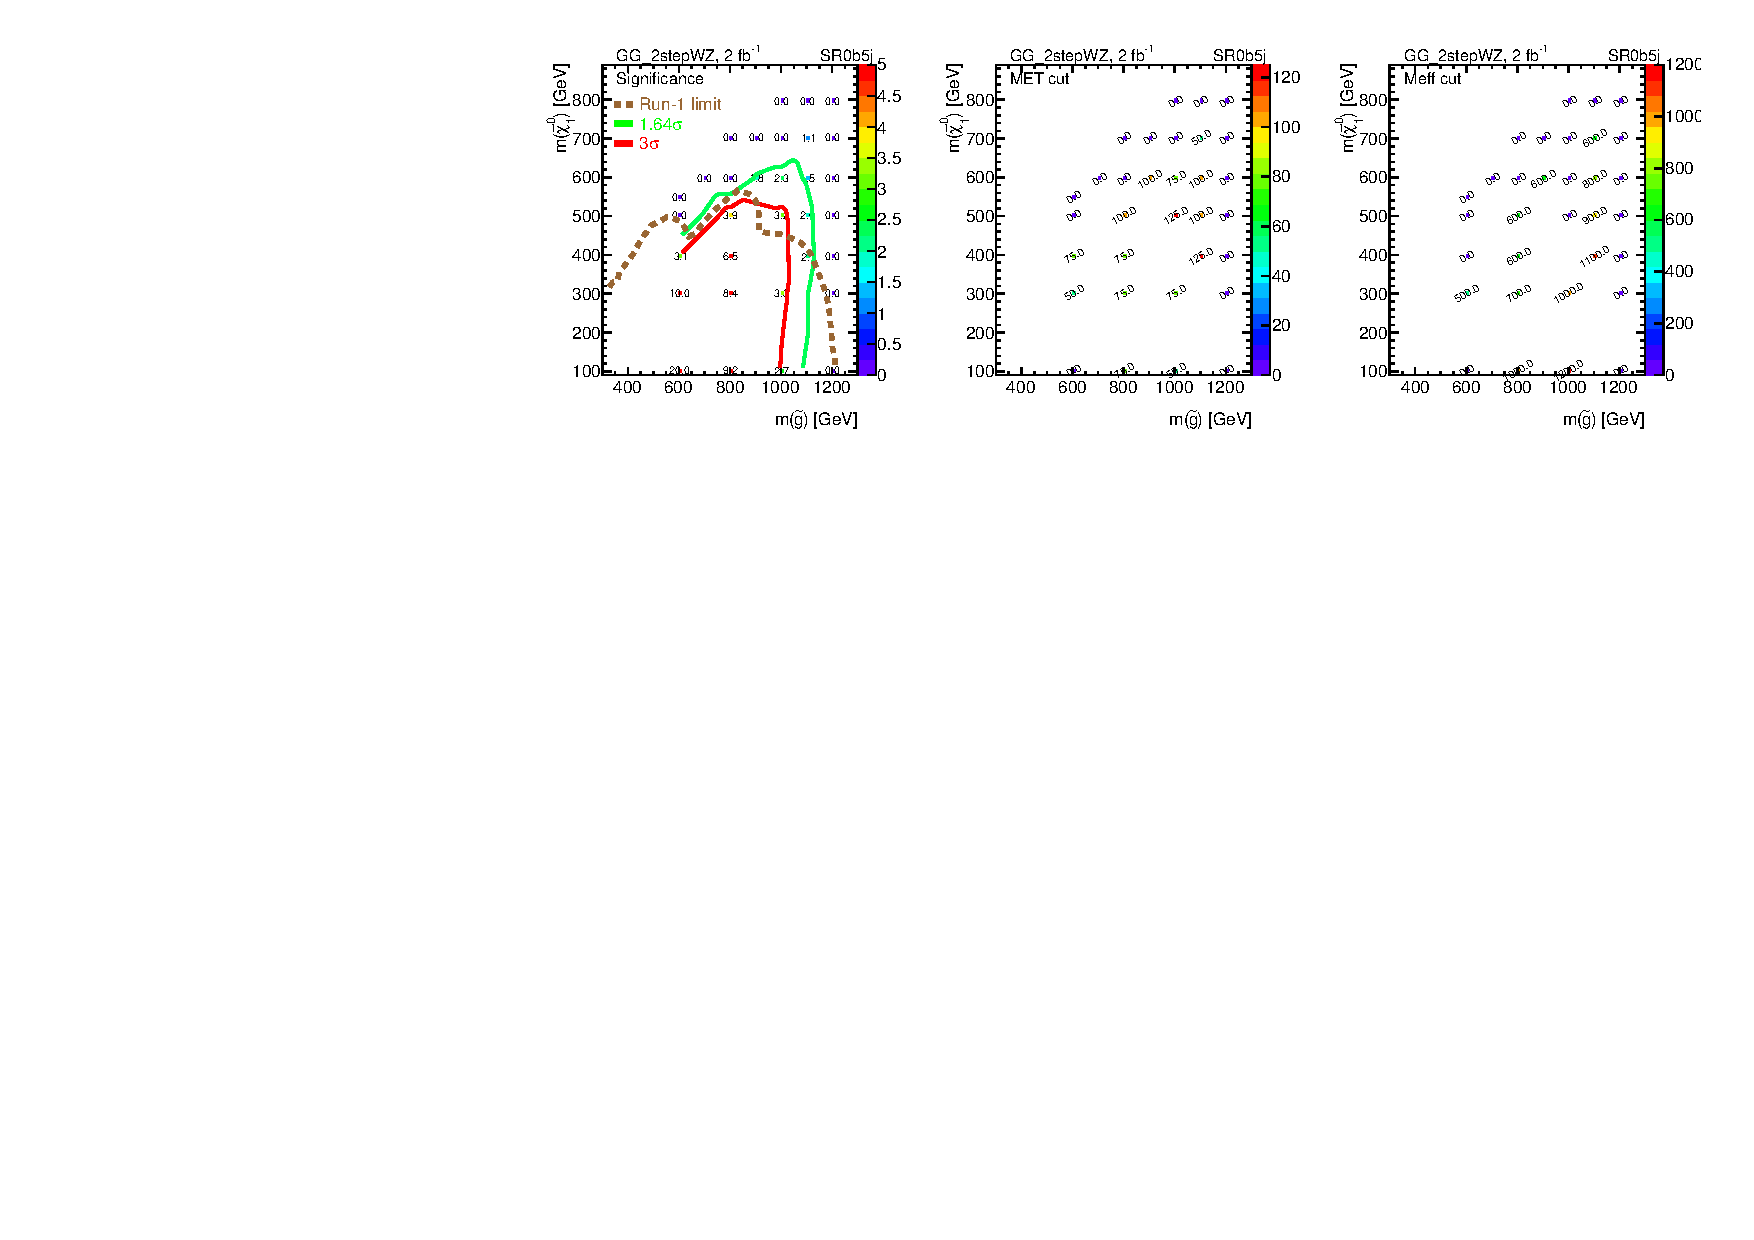
\includegraphics[width=\textwidth]{OPTIMIZATION/Optimiz_SR0b5j_2fb.pdf}
%  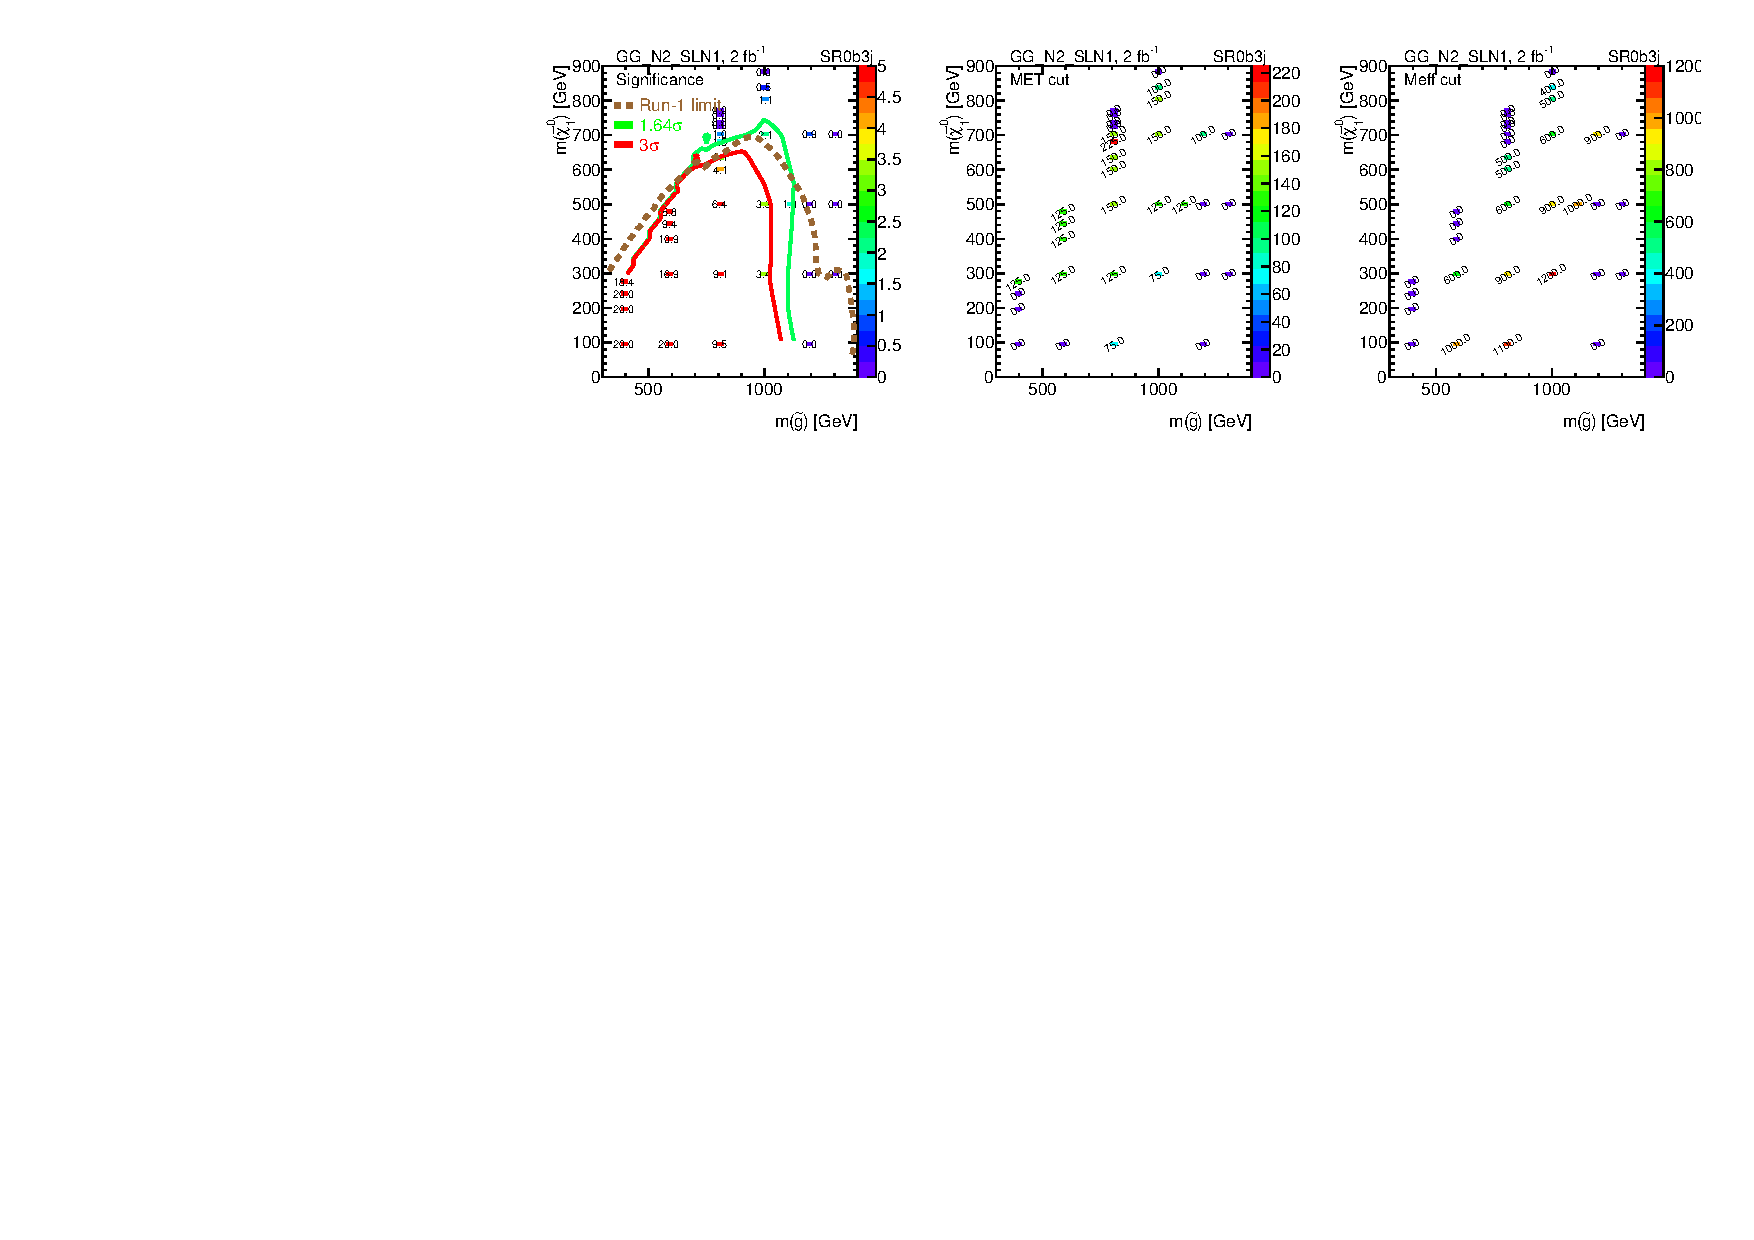
\includegraphics[width=\textwidth]{OPTIMIZATION/Optimiz_SR0b3j_2fb.pdf}
%\caption{Maximum discovery significance (left) for 2~\ifb\, as well as the $\met$ (center) and $\meff$ (right) cuts needed to maximize the significance for SR0b5j in the $\gluino\gluino$ 2-step grid (top) and SR0b3j in the $\gluino\gluino$ 1-step grid (bottom). The Run-1 limits in those models are shown with a brown line.}
%\label{fig:OptimSig2}
%\end{figure}


\subsection{Signal regions}
 
The definition of the exact SR was done as a good compromise across the signal grids shown in 
Figure~\ref{fig:OptimSig1} with a single ($\met$, $\meff$) configuration. 
Tables~\ref{tab:SRdef2}-\ref{tab:SRdef4} show the optimized signal region definitions for scenarios with 2, 3 and 4~\ifb\, respectively. 
The final SR to be used for the 2015 analysis was determined by the luminosity available at the end of the data-taking period: 
if less than 2.5~\ifb\ had been available for analysis after GRL, we would have used the SRs for the 2~\ifb\ scenario; 
if more than 3.5~\ifb\ had been available, we would have used the SRs for the 4~\ifb\ scenario. 
But with the 3.2~\ifb\ eventually collected, we used the definitions corresponding to the intermediate scenario of 3~\ifb.
Figures~\ref{fig:OptimSig2} and \ref{fig:OptimSig4} show the significance values obtained for those signal regions in the SUSY models considered, 
with the 1.64$\sigma$ discovery contours extending beyond the Run-1 exclusions, even achieving a 3$\sigma$ sensitivity in certain regions of the mass parameter space.
 
 
\begin{table}[htb!]
\caption{Signal regions definition for the 2~\ifb\ scenario (to be used for $L <2.5$~fb$^{-1}$). The two leading leptons are required to have \pt~$>$~20~\GeV.}
\hspace{0.5cm}
\label{tab:SRdef2}
\centering
\begin{tabular}{|c|c|c|c|c|c|}
\hline 
\hline
Signal region  &  $N_{\rm{lept}}$   & $N_{b\rm{-jets}}^{20}$    & $N_{\rm{jets}}^{50}$  & \met\ [GeV] & \meff\ [GeV]   \\
\hline\hline
SR3b     &   $\ge$2  &   $\ge$3  &  - & $>$100 & $>$600   \\
\hline
SR1b     &  $\ge$2  &    $\ge$1  &  $\ge$4 &  $>$125 & $>$500 \\
\hline
SR0b5j &  $\ge$2  &    $==$0 &  $\ge$5 &  $>$100 & $>$600 \\
\hline
SR0b3j &  $\ge$3  &    $==$0 &  $\ge$3 &  $>$150 & $>$500 \\
\hline\hline
\end{tabular}
\end{table}

\begin{table}[htb!]
\caption{Signal regions definition for the 3~\ifb\ scenario (to be used for $2.5 \leq L <3.5$~fb$^{-1}$), 
the one eventually used in this analysis. The two leading leptons are required to have \pt~$>$~20~\GeV.}
\hspace{0.5cm}
\label{tab:SRdef3}
\centering
\begin{tabular}{|c|c|c|c|c|c|}
\hline 
\hline
Signal region  &  $N_{\rm{lept}}$   & $N_{b\rm{-jets}}^{20}$    & $N_{\rm{jets}}^{50}$  & \met\ [GeV] & \meff\ [GeV]   \\
\hline\hline
SR3b     &   $\ge$2  &   $\ge$3  &  - & $>$125 & $>$650   \\
\hline
SR1b     &  $\ge$2  &    $\ge$1  &  $\ge$4 &  $>$150 & $>$550 \\
\hline
SR0b5j &  $\ge$2  &    $==$0 &  $\ge$5 &  $>$125 & $>$650 \\
\hline
SR0b3j &  $\ge$3  &    $==$0 &  $\ge$3 &  $>$200 & $>$550 \\
\hline\hline
\end{tabular}
\end{table}

\begin{table}[htb!]
\caption{Signal regions definition for the 4~\ifb\ scenario (to be used for $L \geq 3.5$~fb$^{-1}$). The two leading leptons are required to have \pt~$>$~20~\GeV.}
\hspace{0.5cm}
\label{tab:SRdef4}
\centering
\begin{tabular}{|c|c|c|c|c|c|}
\hline 
\hline
Signal region  &  $N_{\rm{lept}}$   & $N_{b\rm{-jets}}^{20}$    & $N_{\rm{jets}}^{50}$  & \met\ [GeV] & \meff\ [GeV]   \\
\hline\hline
SR3b     &   $\ge$2  &   $\ge$3  &  - & $>$125 & $>$700   \\
\hline
SR1b     &  $\ge$2  &    $\ge$1  &  $\ge$4 &  $>$150 & $>$600 \\
\hline
SR0b5j &  $\ge$2  &    $==$0 &  $\ge$5 &  $>$125 & $>$700 \\
\hline
SR0b3j &  $\ge$3  &    $==$0 &  $\ge$3 &  $>$200 & $>$600 \\
\hline\hline
\end{tabular}
\end{table}

\begin{figure}[!htb]
\centering
  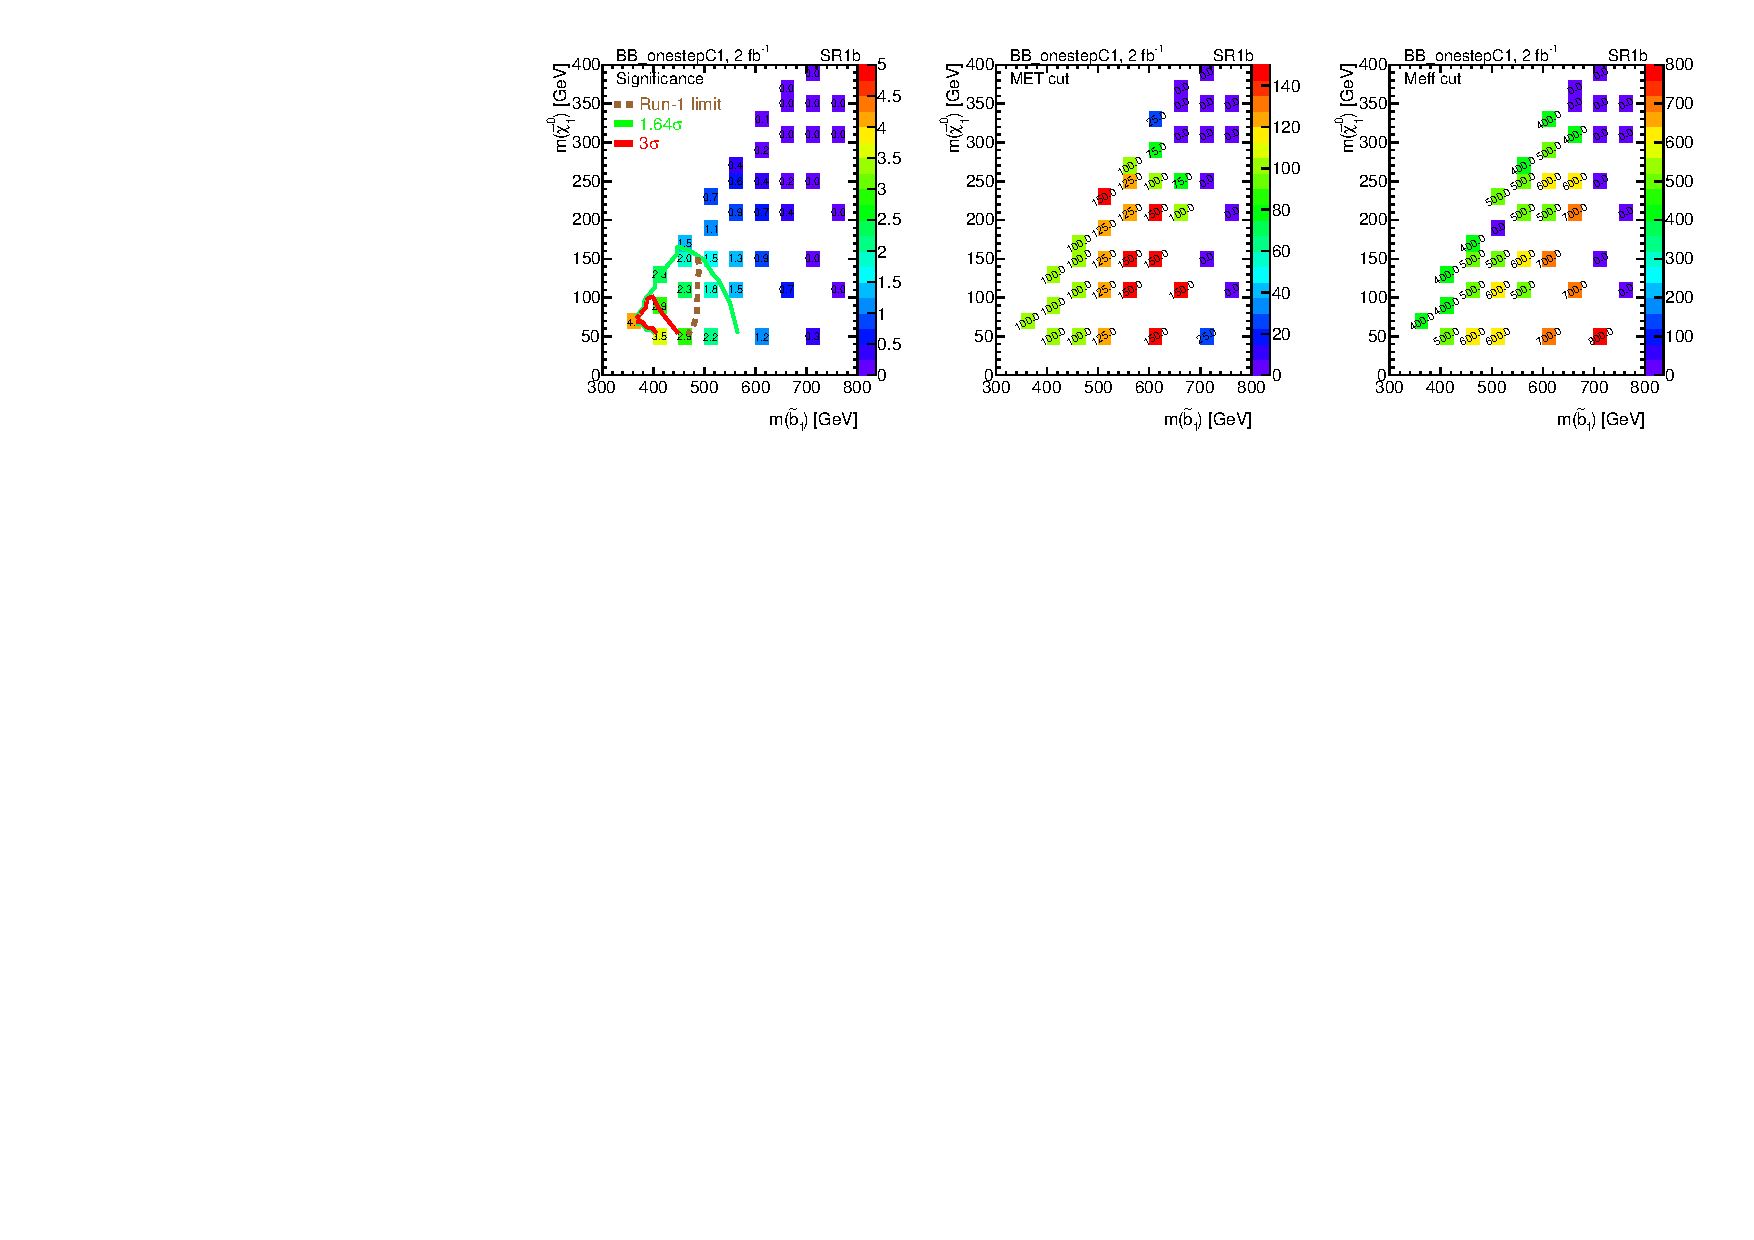
\includegraphics[width=0.9\textwidth]{OPTIMIZATION/Optimiz_SR1b_2fb.pdf}
  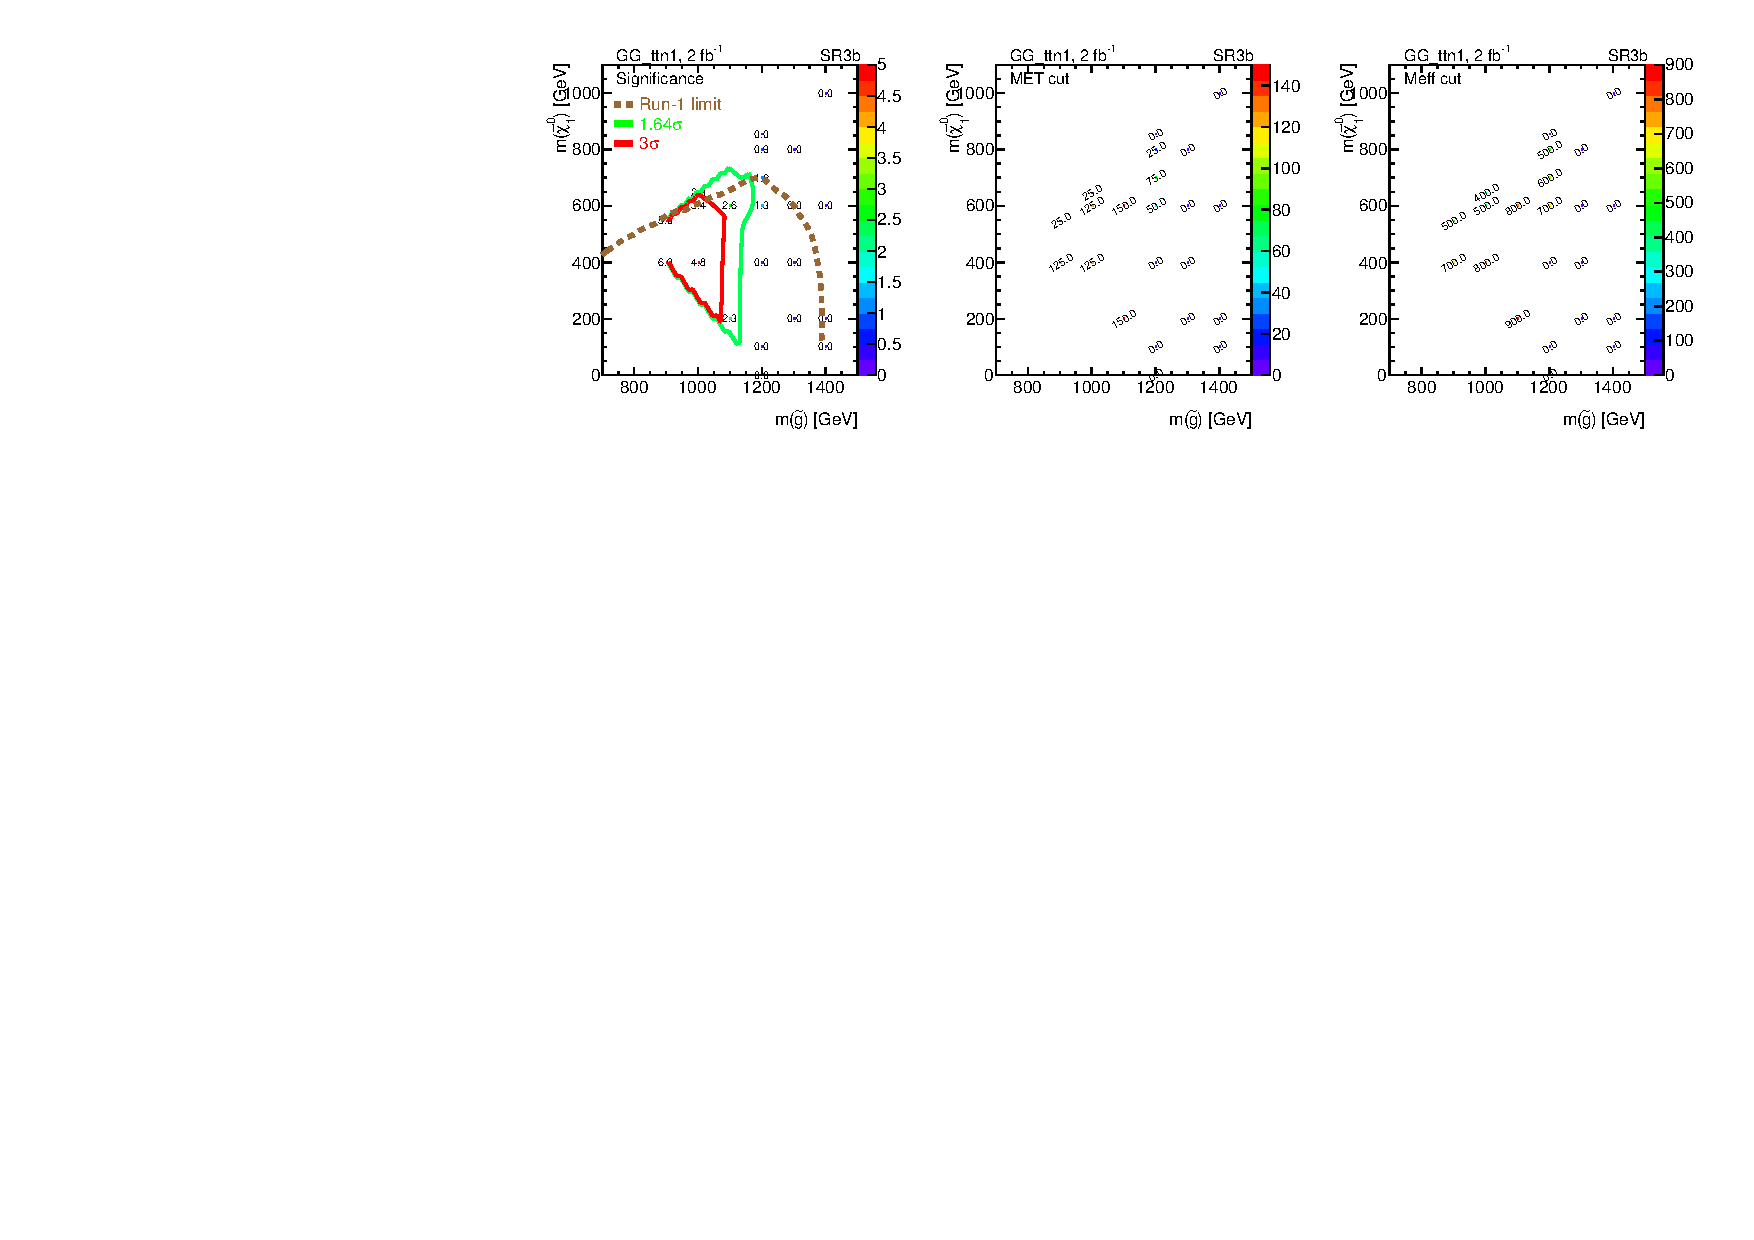
\includegraphics[width=0.9\textwidth]{OPTIMIZATION/Optimiz_SR3b_2fb.pdf}
  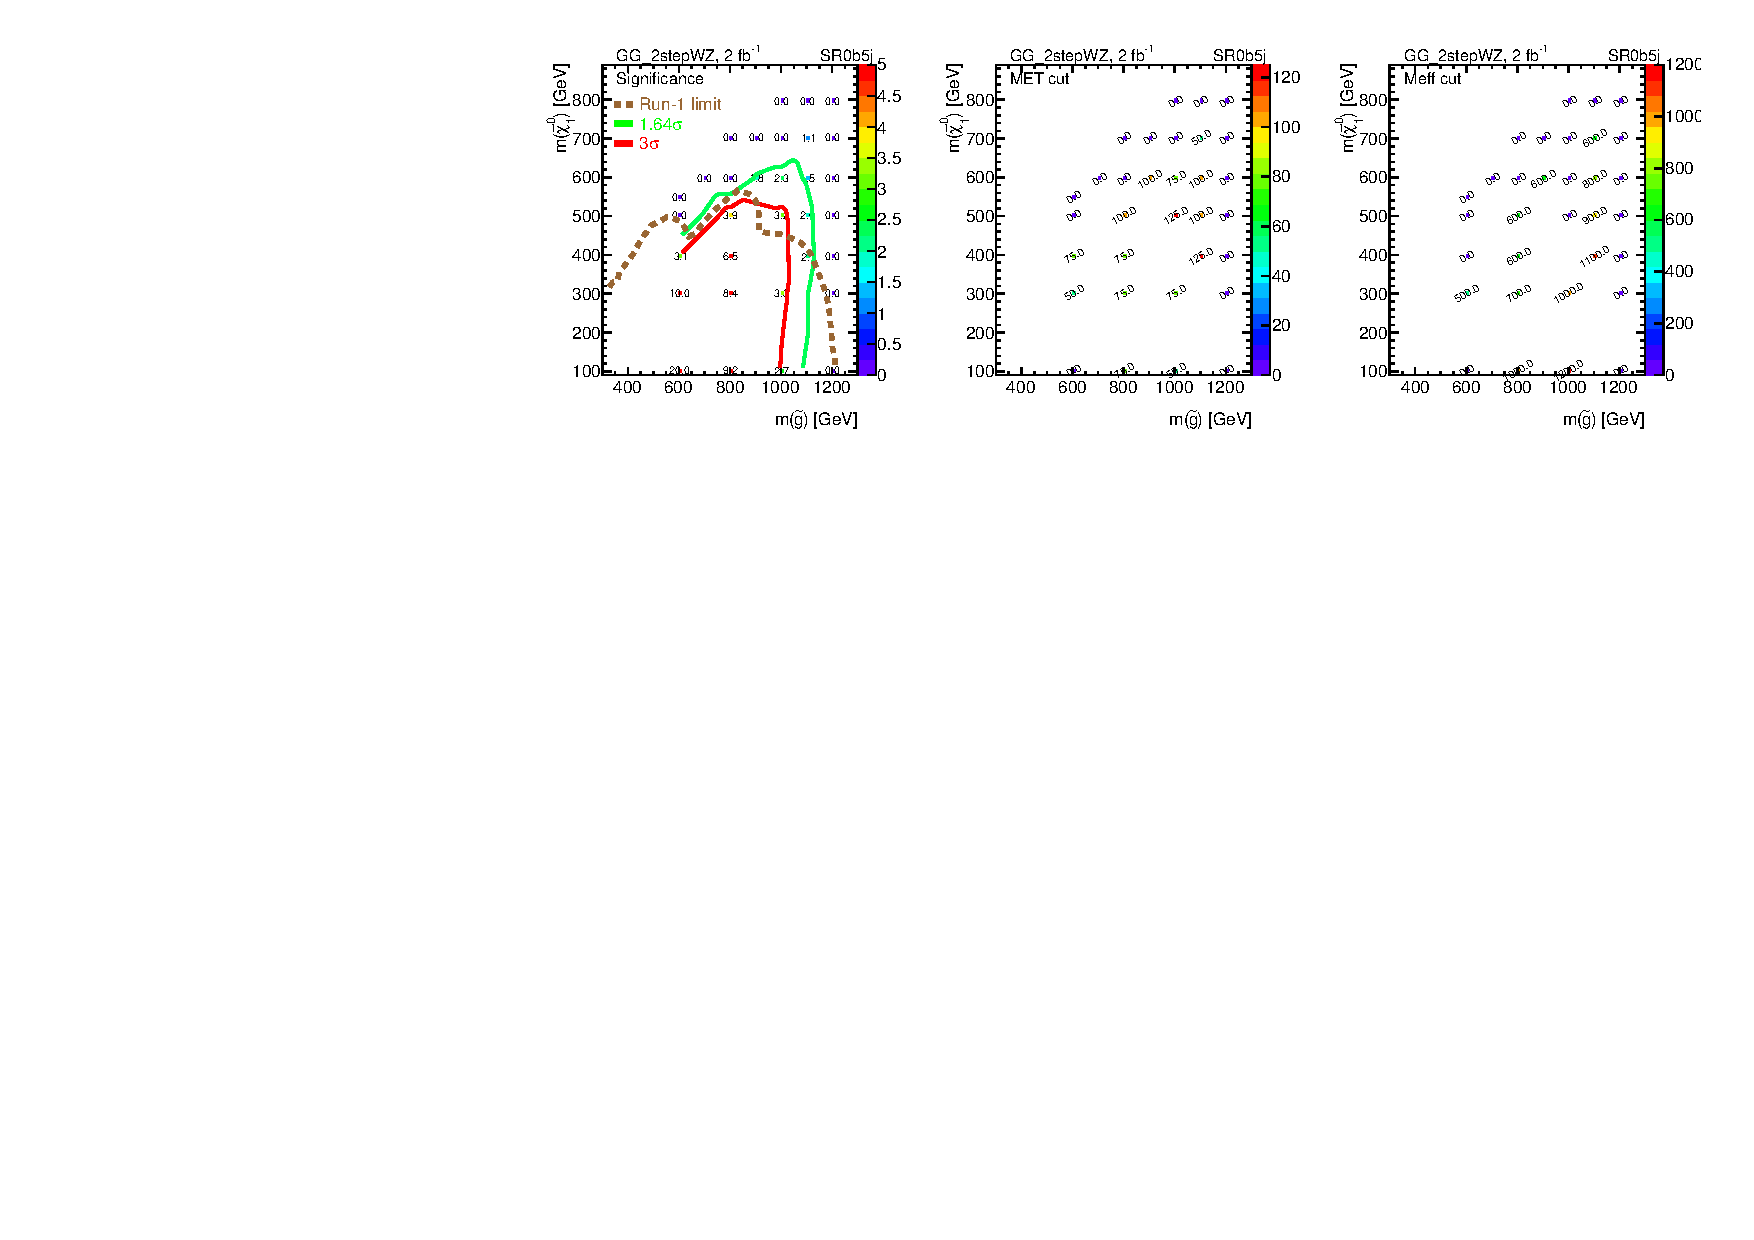
\includegraphics[width=0.9\textwidth]{OPTIMIZATION/Optimiz_SR0b5j_2fb.pdf}
  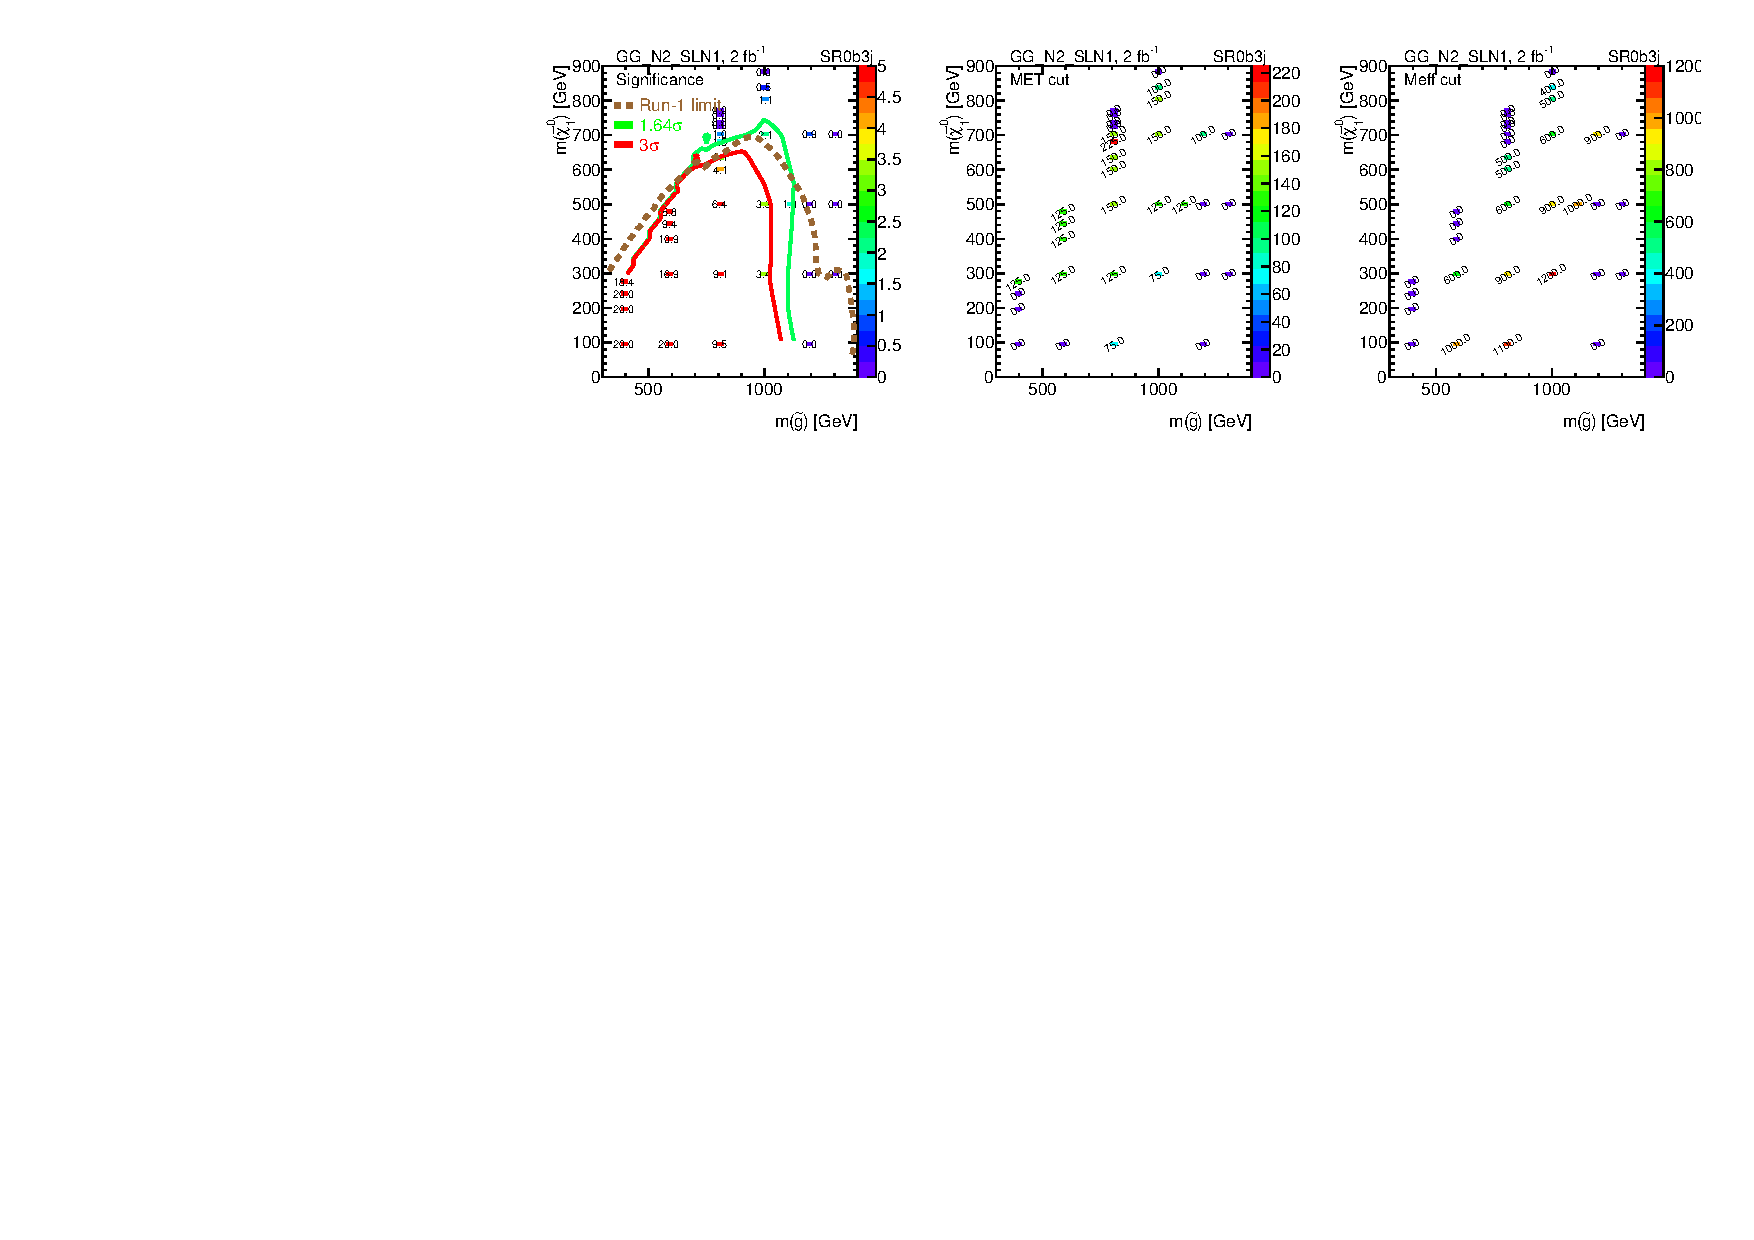
\includegraphics[width=0.9\textwidth]{OPTIMIZATION/Optimiz_SR0b3j_2fb.pdf}
  \caption{Maximum discovery significance (left) for 2~\ifb, as well as the $\met$ (center) and $\meff$ (right) cuts needed to maximize the significance for: (from top to bottom) SR1b in the $\sbot\sbot^*\to t\bar t\tilde\chi_1^+\tilde\chi_1^-$ grid, SR3b in the $\gluino\gluino\to t\bar tt\bar t\ninoone\ninoone$ grid, SR0b5j in the $\gluino\gluino$ with $\gluino\to q\bar{q}'WZ\ninoone$ grid and SR0b3j in the $\gluino\gluino$ with $\gluino\to q\bar{q}(\ell\ell/\ell\nu)\ninoone$ grid. The Run-1 limits in those models are shown with a brown line, and the 1.64$\sigma$ and 3$\sigma$ discovery contours from the proposed signal regions are shown in green and red, respectively.}
\label{fig:OptimSig1}
\end{figure}



\begin{figure}[!htb]
\centering
  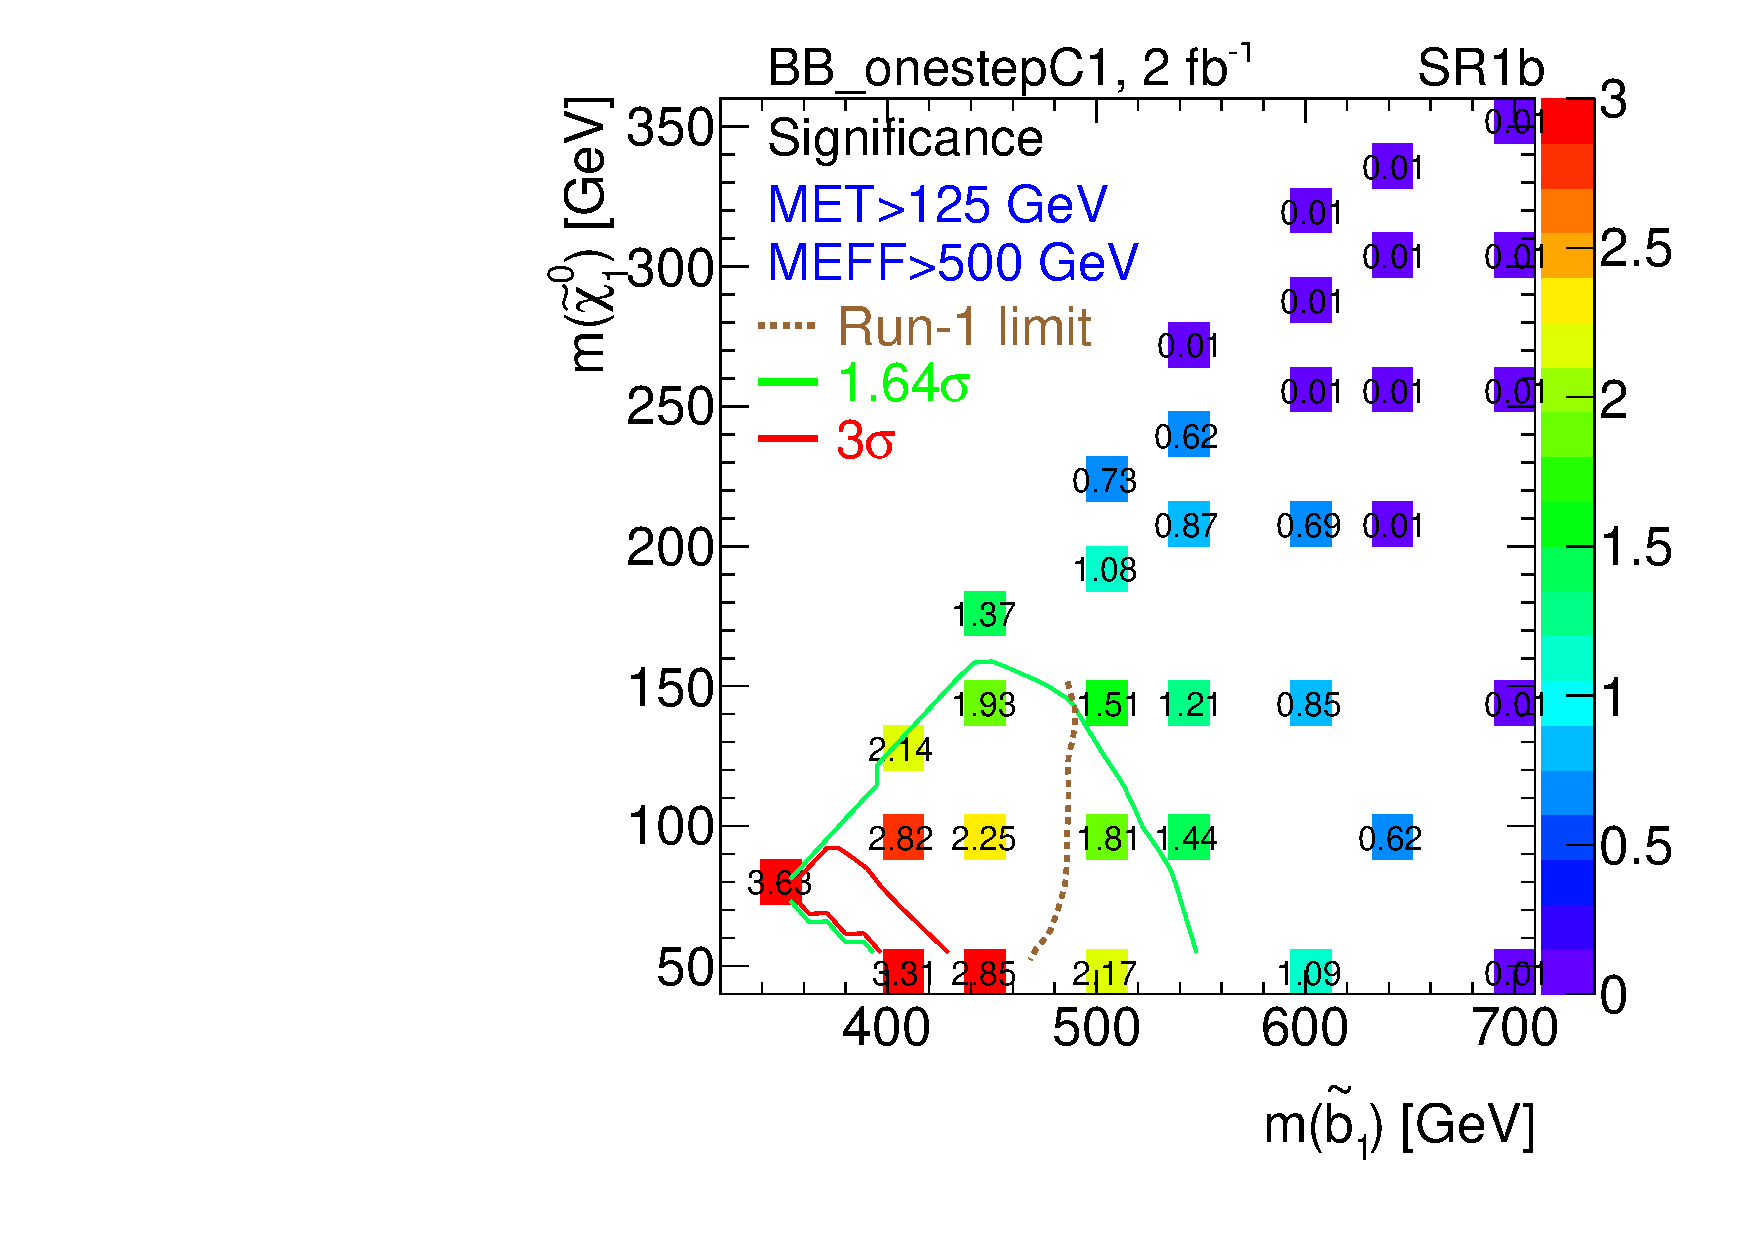
\includegraphics[width=0.4\textwidth]{OPTIMIZATION/Optimiz_SR1b_2fb_125_500.pdf}
  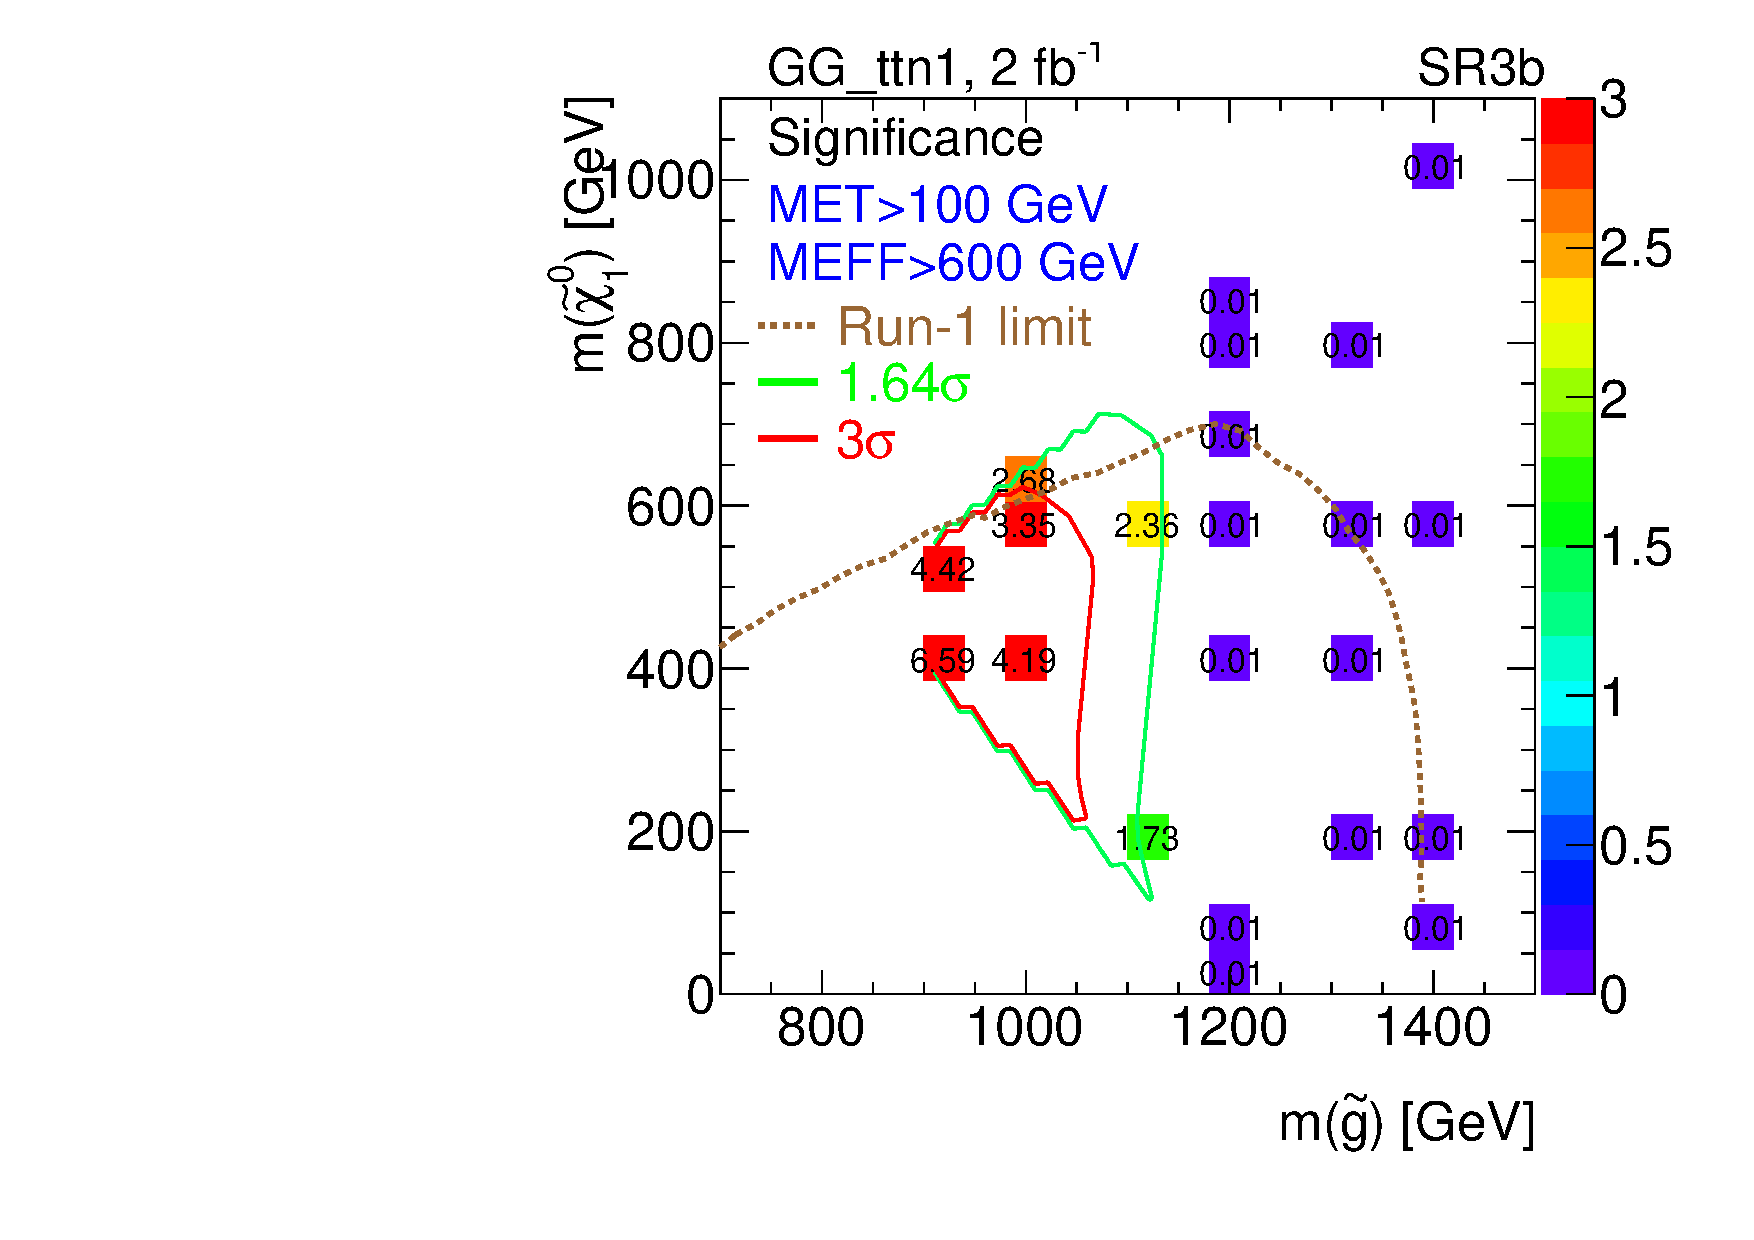
\includegraphics[width=0.4\textwidth]{OPTIMIZATION/Optimiz_SR3b_2fb_100_600.pdf}\\
  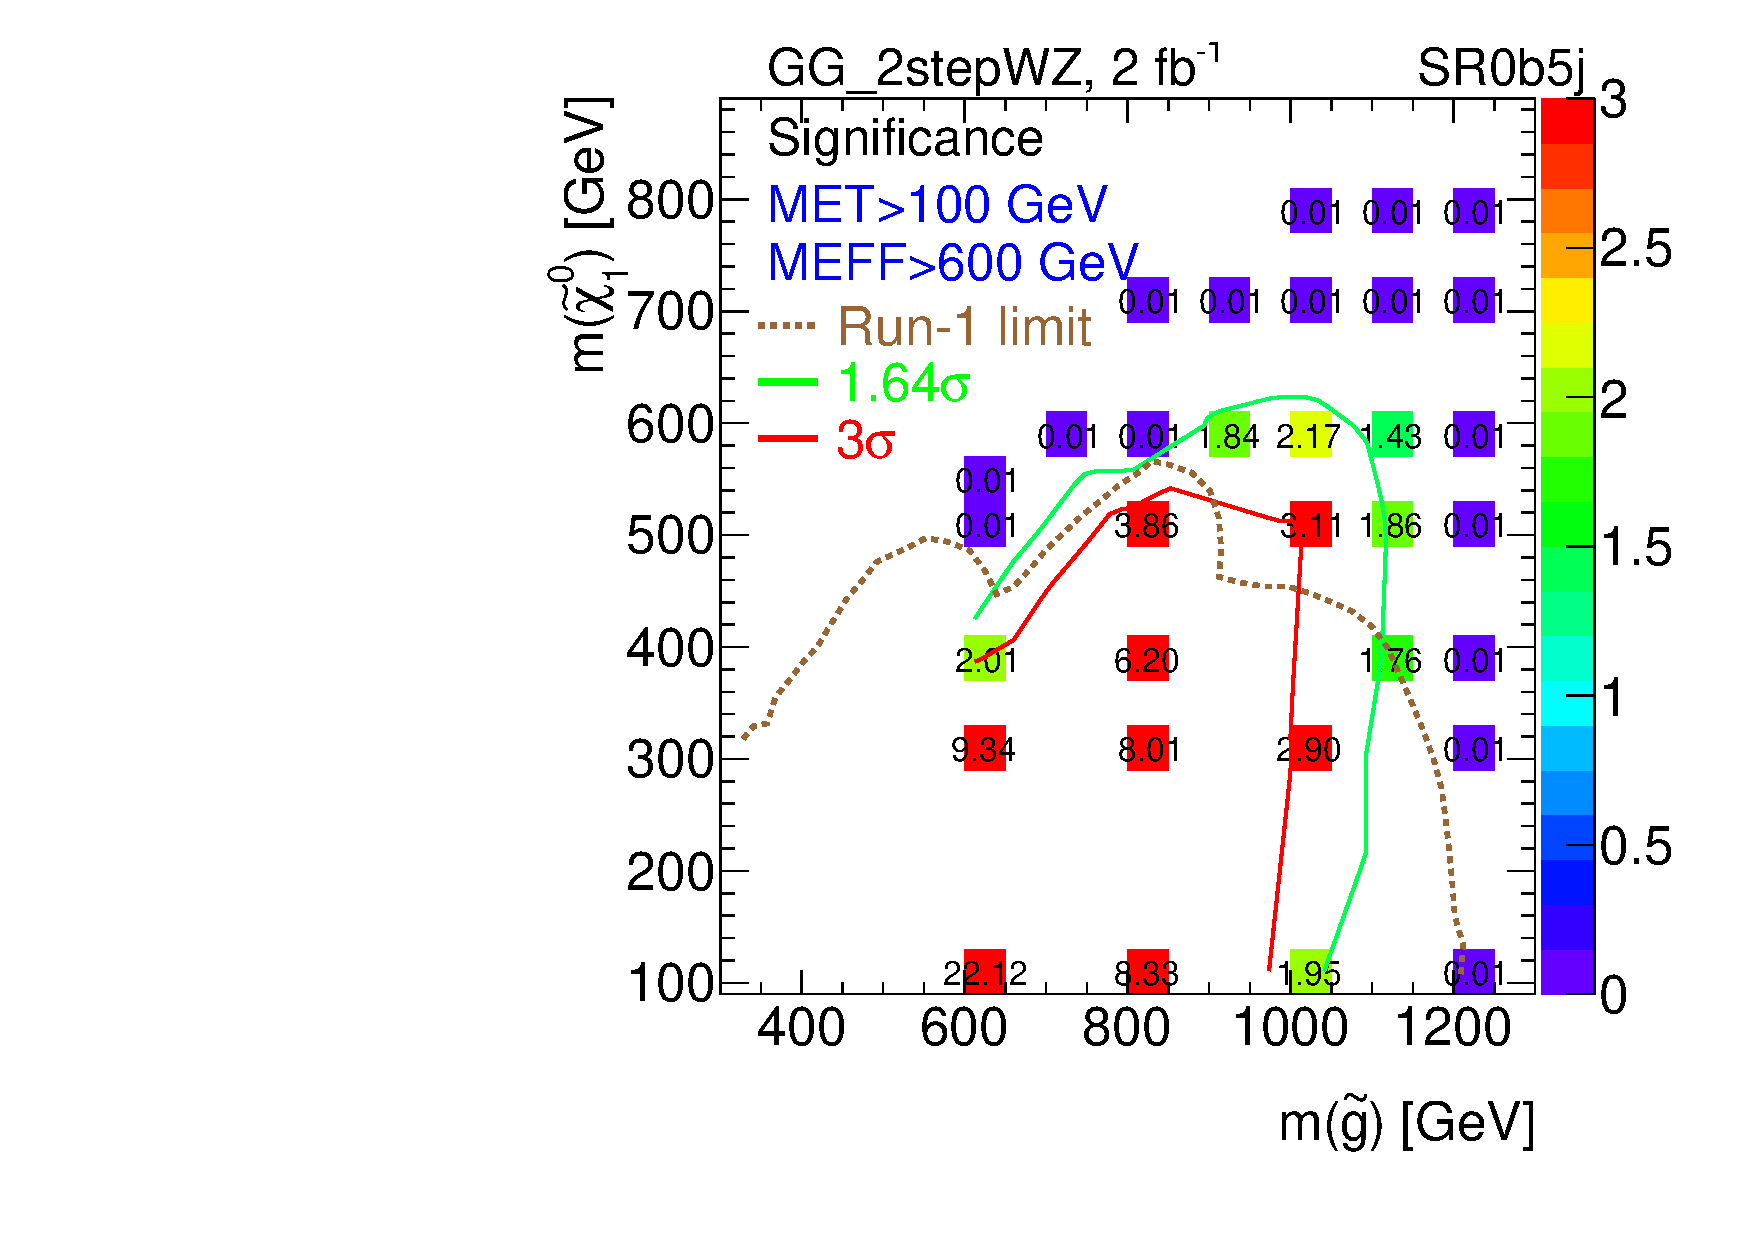
\includegraphics[width=0.4\textwidth]{OPTIMIZATION/Optimiz_SR0b5j_2fb_100_600.pdf}
  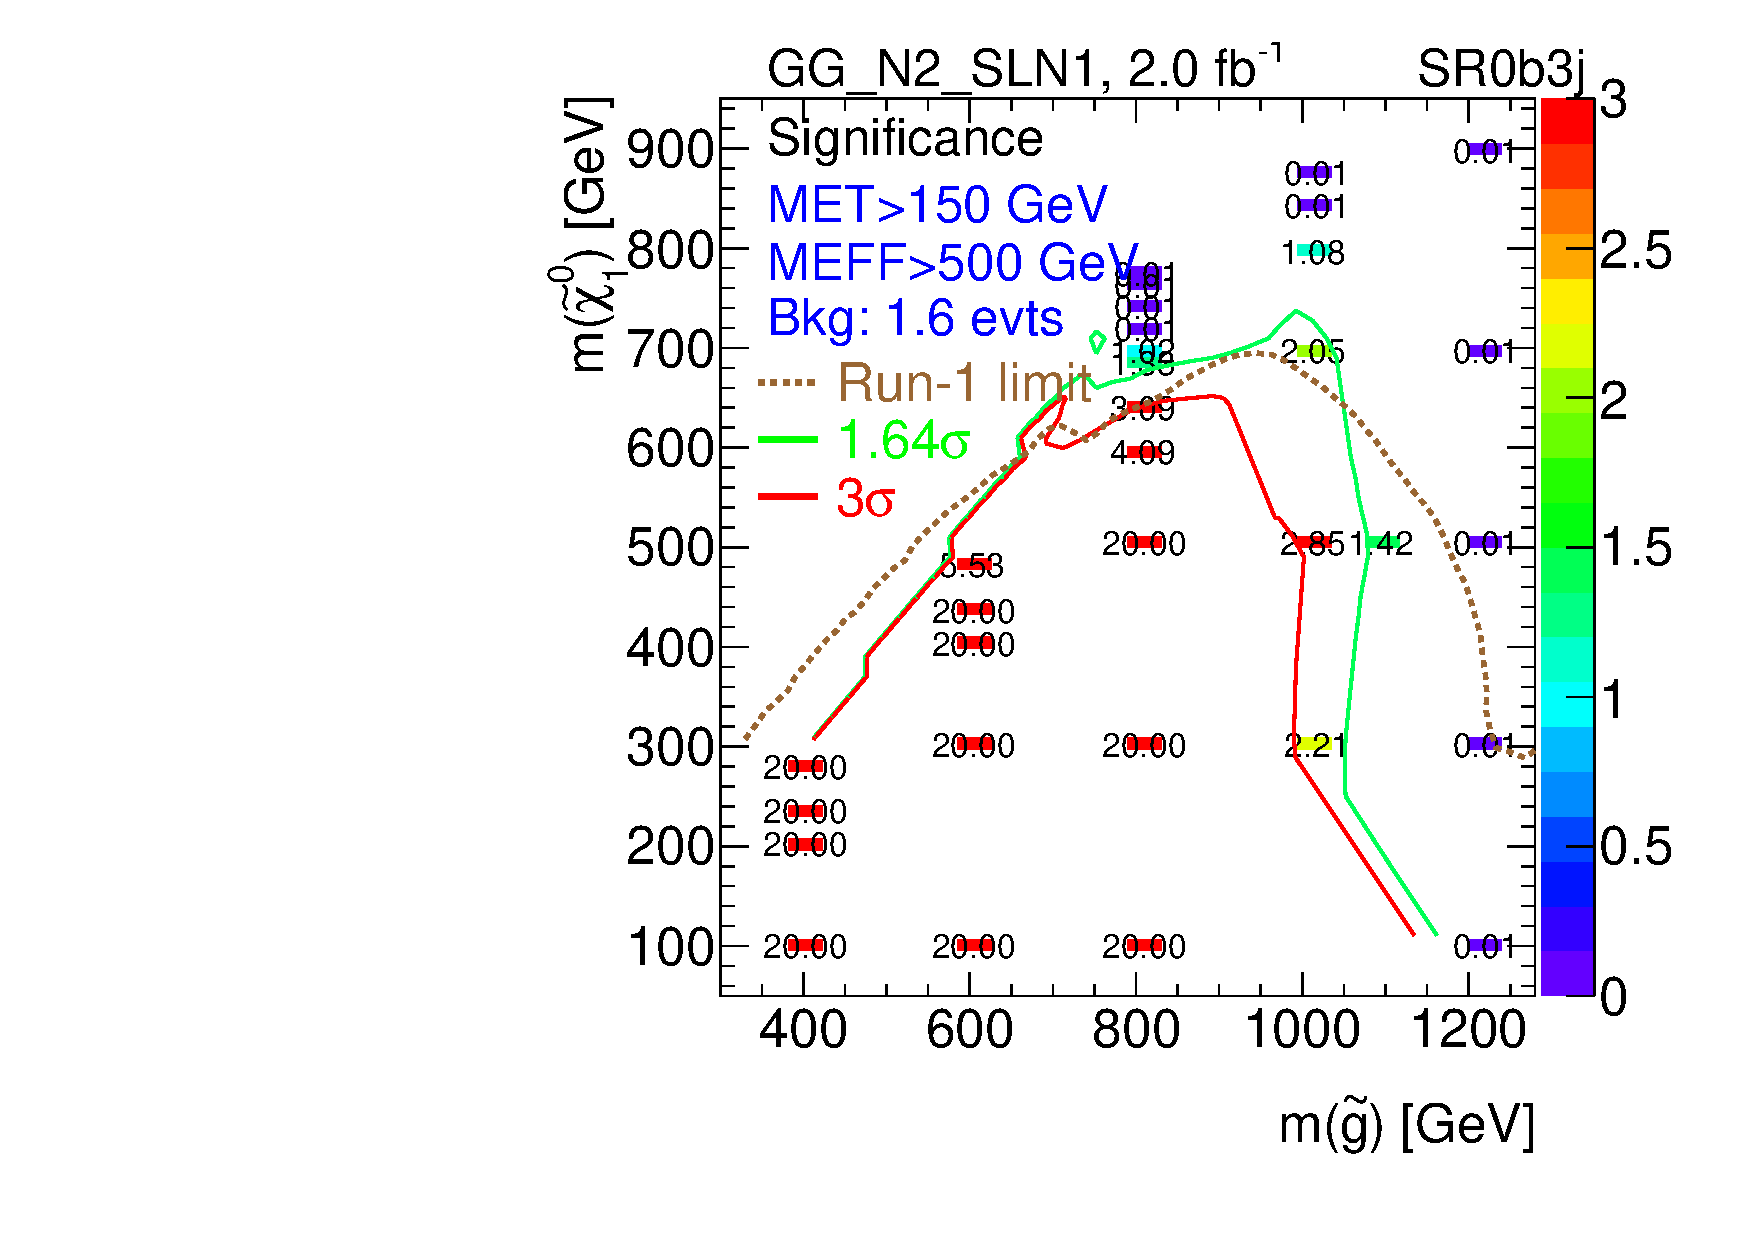
\includegraphics[width=0.4\textwidth]{OPTIMIZATION/Optimiz_SR0b3j_2fb_150_500.pdf}
  \caption{Discovery significance for the SRs defined in Table~\ref{tab:SRdef2} (2~\ifb) for SR1b in the $\sbot\sbot^*\to t\bar t\tilde\chi_1^+\tilde\chi_1^-$ grid (top left), SR3b in the $\gluino\gluino\to t\bar tt\bar t\ninoone\ninoone$ grid (top right), SR0b5j in the $\gluino\gluino$ with $\gluino\to q\bar{q}'WZ\ninoone$ grid (bottom left) and SR0b3j in the $\gluino\gluino$ with $\gluino\to q\bar{q}(\ell\ell/\ell\nu)\ninoone$ grid (bottom right). The Run-1 limits in those models are shown with a brown line, and the 1.64$\sigma$ and 3$\sigma$ discovery contours from the proposed signal regions are shown in green and red, respectively.}
\label{fig:OptimSig2}
\end{figure}


\begin{figure}[!htb]
\centering
  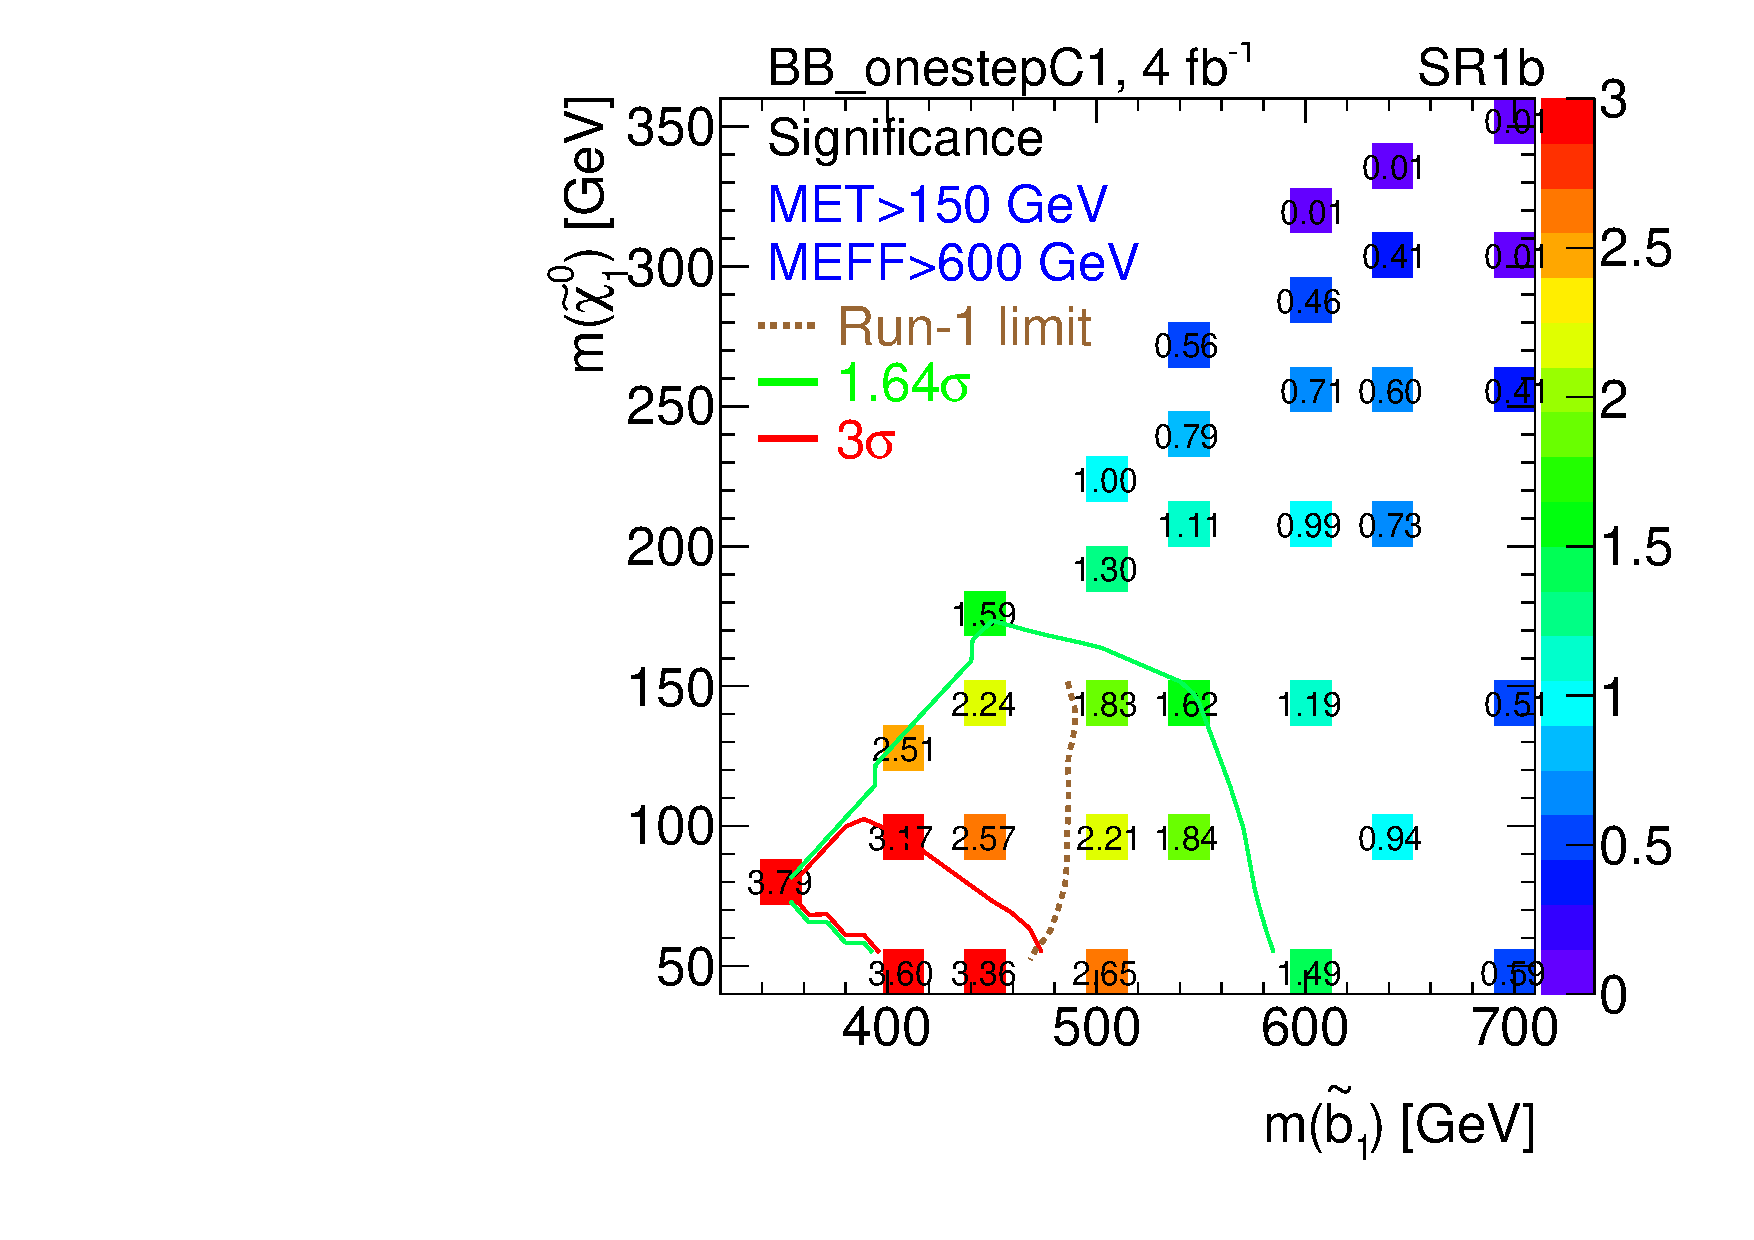
\includegraphics[width=0.4\textwidth]{OPTIMIZATION/Optimiz_SR1b_4fb_150_600.pdf}
  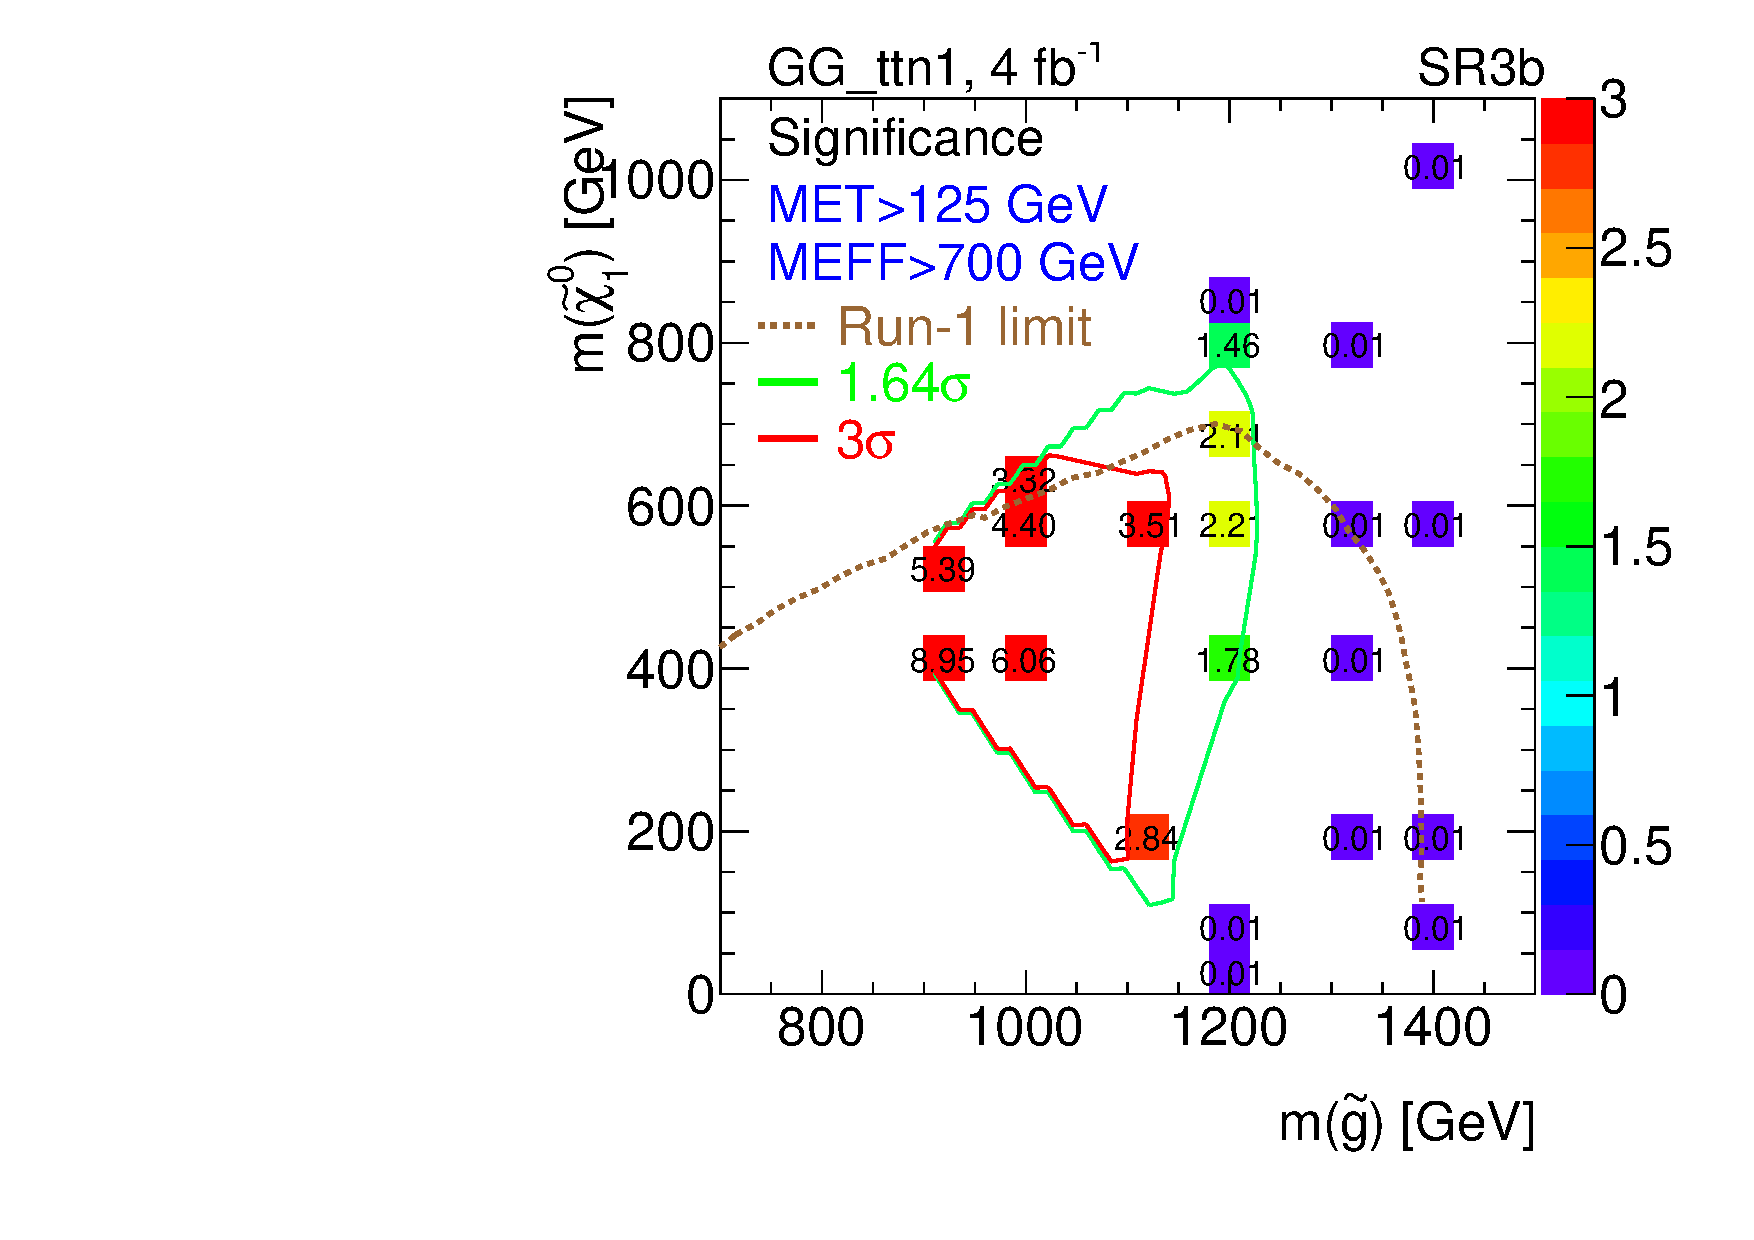
\includegraphics[width=0.4\textwidth]{OPTIMIZATION/Optimiz_SR3b_4fb_125_700.pdf}\\
  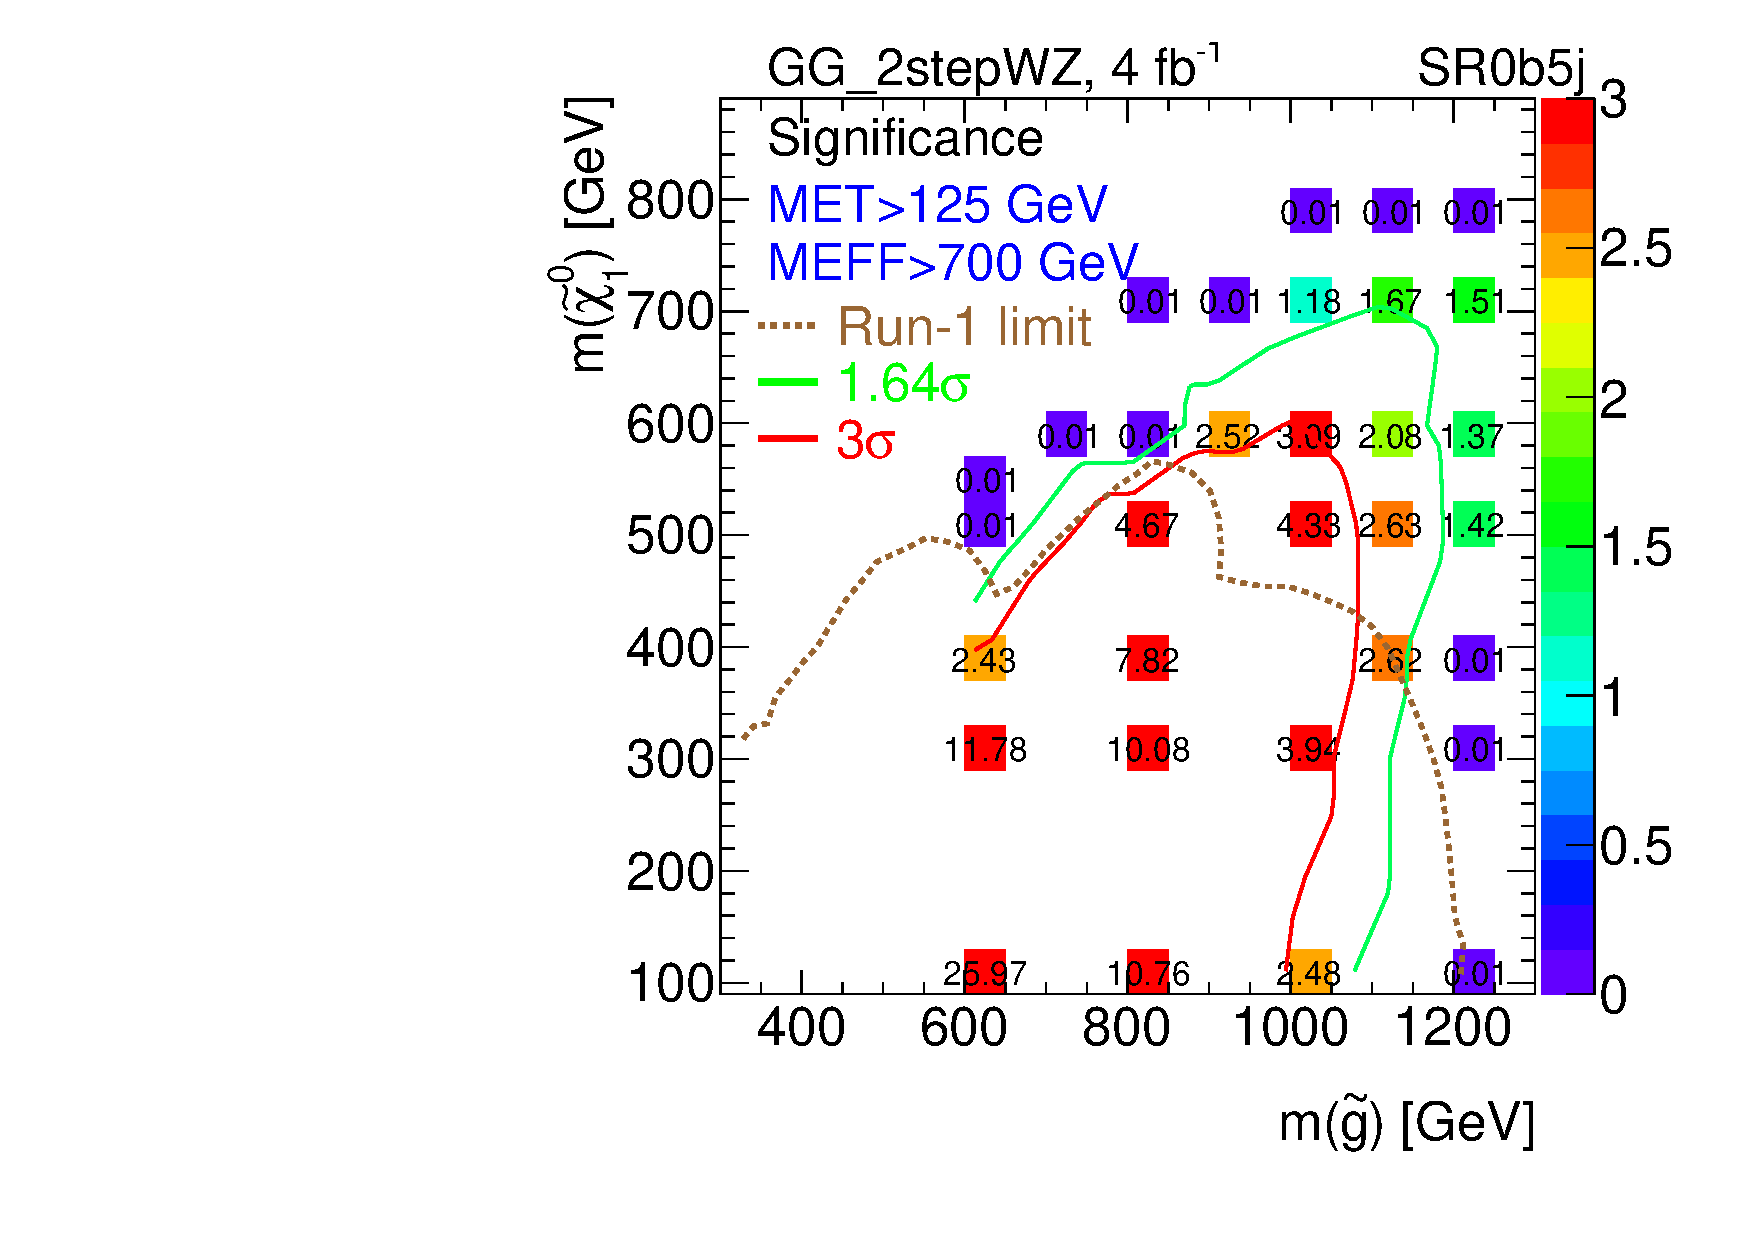
\includegraphics[width=0.4\textwidth]{OPTIMIZATION/Optimiz_SR0b5j_4fb_125_700.pdf}
  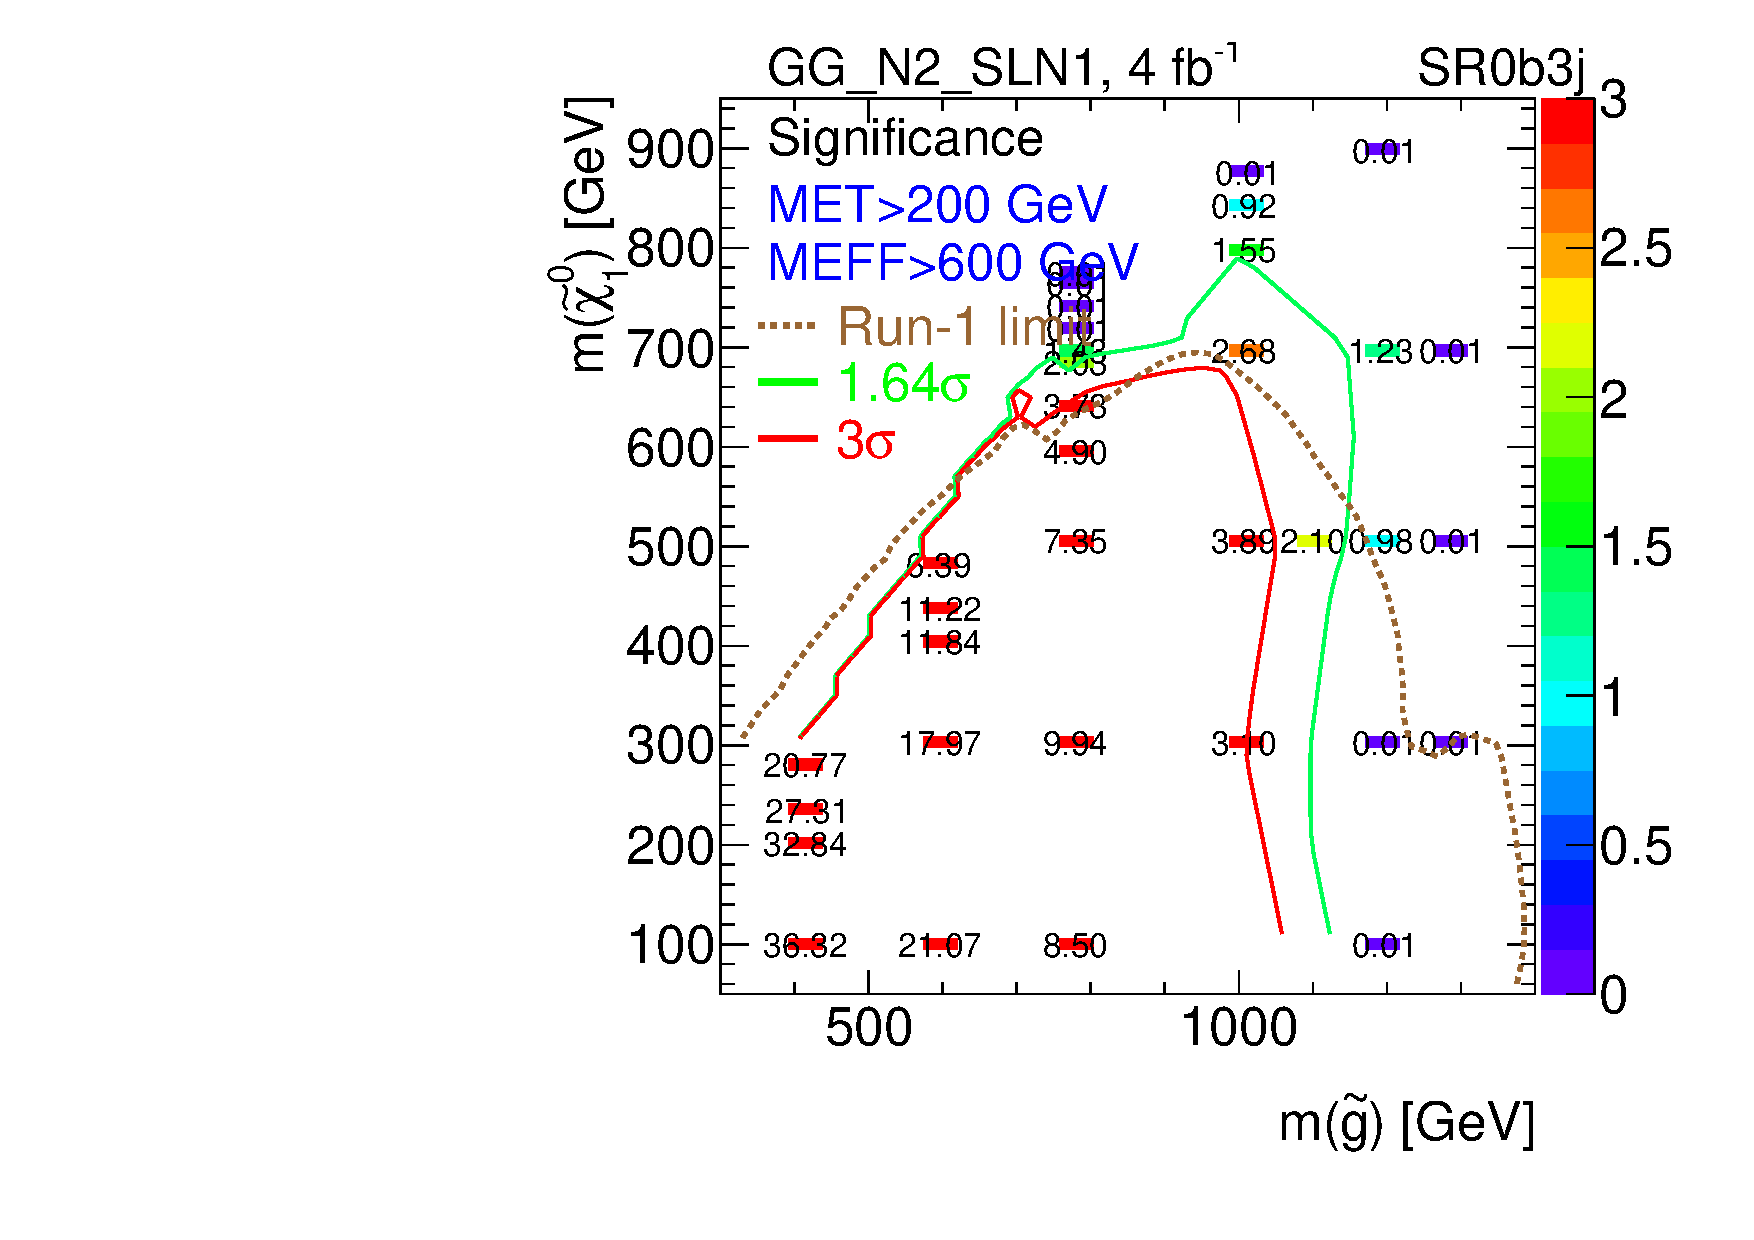
\includegraphics[width=0.4\textwidth]{OPTIMIZATION/Optimiz_SR0b3j_4fb_200_600.pdf}
  \caption{Discovery significance for the SRs defined in Table~\ref{tab:SRdef4} (4~\ifb) for SR1b in the $\sbot\sbot^*\to t\bar t\tilde\chi_1^+\tilde\chi_1^-$ grid (top left), SR3b in the $\gluino\gluino\to t\bar tt\bar t\ninoone\ninoone$ grid (top right), SR0b5j in the $\gluino\gluino$ with $\gluino\to q\bar{q}'WZ\ninoone$ grid (bottom left) and SR0b3j in the $\gluino\gluino$ with $\gluino\to q\bar{q}(\ell\ell/\ell\nu)\ninoone$ grid (bottom right). The Run-1 limits in those models are shown with a brown line, and the 1.64$\sigma$ and 3$\sigma$ discovery contours from the proposed signal regions are shown in green and red, respectively.}
\label{fig:OptimSig4}
\end{figure}


%\FloatBarrier



%\section{Background estimation}
%\label{sec:bkg}
%Two main sources of SM background can be distinguished in this analysis. 
The first category is the reducible or detector background which includes 
events containing electrons with mis-measured charge, mainly from the production of top quark pairs, and events 
containing at least one non-prompt or fake lepton (FNP), which mainly originate from hadron decays in events containing 
top quarks, $W$ or $Z$ bosons. Data-driven methods used for the estimation
of this background are described in Section~\ref{sec:DD_bkg}. The second category consists of events 
with two same-sign prompt leptons or at least three prompt leptons and is 
estimated using the MC samples described in Section~\ref{sec:dataMC}. 
Since diboson and $\ttbar V$ events are the main backgrounds in the signal regions, 
dedicated validation regions (VR) with an enhanced contribution from these processes 
are defined to verify the background predictions from the simulation (see Section~\ref{sec:valid}).


\subsection{Detector background estimation methods} 
\label{sec:DD_bkg}

Background events due to charge mis-identification concerns only the electron. The probability of mis-identifying the 
charge of a muon is checked in both data and MC simulation, and found to be negligible in the kinematic range relevant to this analysis.
The contribution of charge-flip events to the SR/VR yields is estimated using the data. 
The electron charge-flip probability is extracted in a $Z/\gamma^{*}\to ee$ data sample using a likelihood fit 
which takes as input the numbers of same-sign and opposite-sign electron pairs observed in a window around the $Z$ mass. 
The charge-flip probability is a free parameter of the fit and is extracted as a function of the electron $\pt$ and $\eta$. 
These probabilities are in the range \textcolor{red}{UPDATE:1--5\%} and \textcolor{red}{UPDATE:0.1--1\%} for the candidate 
and signal electrons respectively.
The event yield of this background in the signal or validation regions is obtained by applying the measured charge-flip probability 
to the data regions with the same kinematic requirements as the signal or validation regions but with opposite-sign lepton pairs. 

The contribution from fake or non-prompt leptons (such as hadrons mis-identified as leptons, 
leptons originating from heavy-flavour decays, and electrons from photon conversions) 
is also estimated from the data with a matrix method similar to that described in Ref.~\cite{SUSY3bjetsRun1}. 
In this method, two types of lepton identification criteria are defined: ``tight'', 
corresponding to the signal lepton criteria described in Section~\ref{sec:selection}, 
and ``loose'', corresponding to candidate leptons after overlap removal. 
The matrix method relates the number of events containing prompt or FNP leptons 
to the number of observed events with tight or loose-not-tight leptons 
using the probability for loose prompt or FNP leptons to satisfy the tight criteria. 
The probability for loose prompt leptons to satisfy the tight selection criteria ($\epsilon$)
is obtained using a $Z/\gamma^*\to\ell\ell$ data sample 
and is modelled as a function of the lepton $\pt$ and $\eta$. 
The probability for loose FNP leptons to satisfy the tight selection criteria (FNP fake rate, $f$) is determined from data 
in SS and three lepton control regions enriched in non-prompt leptons originating from heavy-flavour decays, mostly coming from 
semileptonic $\ttbar$ events. This region contains events with at least one $b$-jet, 
one well-isolated ``tag'' muon, and an additional loose electron or muon on which the measurement is performed. 
The efficiencies are measured as function of \pt ($\eta$ binning is also used for low \pt muons) 
after subtracting the small contribution from prompt lepton processes. 

\textcolor{red}{[UPDATE: rewrite/inflate this paragraph]}The estimated FNP yields in the SRs are consistent with those 
predicted by two alternative methods: the first one relies on MC simulation of processes with FNP leptons or charge-flipped electrons 
($\ttbar$, $V$+jets)~\cite{paperSS3L,ATLAS-CONF-2012-151}, 
corrected to match the observed data in dedicated control regions. 
The second method relies on data events with only one lepton, which are the processes leading to FNP leptons, 
to extrapolate from low-\met\ control regions to the SRs.

%The data-driven background estimates are cross-checked with an MC-based technique. 
%In this method, the contributions from processes with FNP leptons and electron charge mis-identification 
%are obtained from MC simulation and normalised to data in dedicated control regions at low jet multiplicity, low $\met$, and 
%either with or without $b$-jets. 
%The normalisation is performed using five multipliers: one to correct 
%the electron charge mis-identification rate, and four to correct the contributions from FNP 
%electrons or muons originating from $b$-jets or light-flavour jets, respectively.
%In addition to the MC samples listed in Section~\ref{sec:dataMC}, this method employs samples of top quark pair production generated with the \POWHEG-Box v2 generator interfaced to \PYTHIA 6.428~\cite{Sjostrand:2006za}, 
%as well as samples of simulated $W$+jets and $Z$+jets events generated with \POWHEG-Box v2 interfaced to \PYTHIA 8.186.

% not the best place, but otherwise it's not well positionned wrt the text...
\begin{figure}[th!]
\centering
\begin{subfigure}[t]{0.49\textwidth}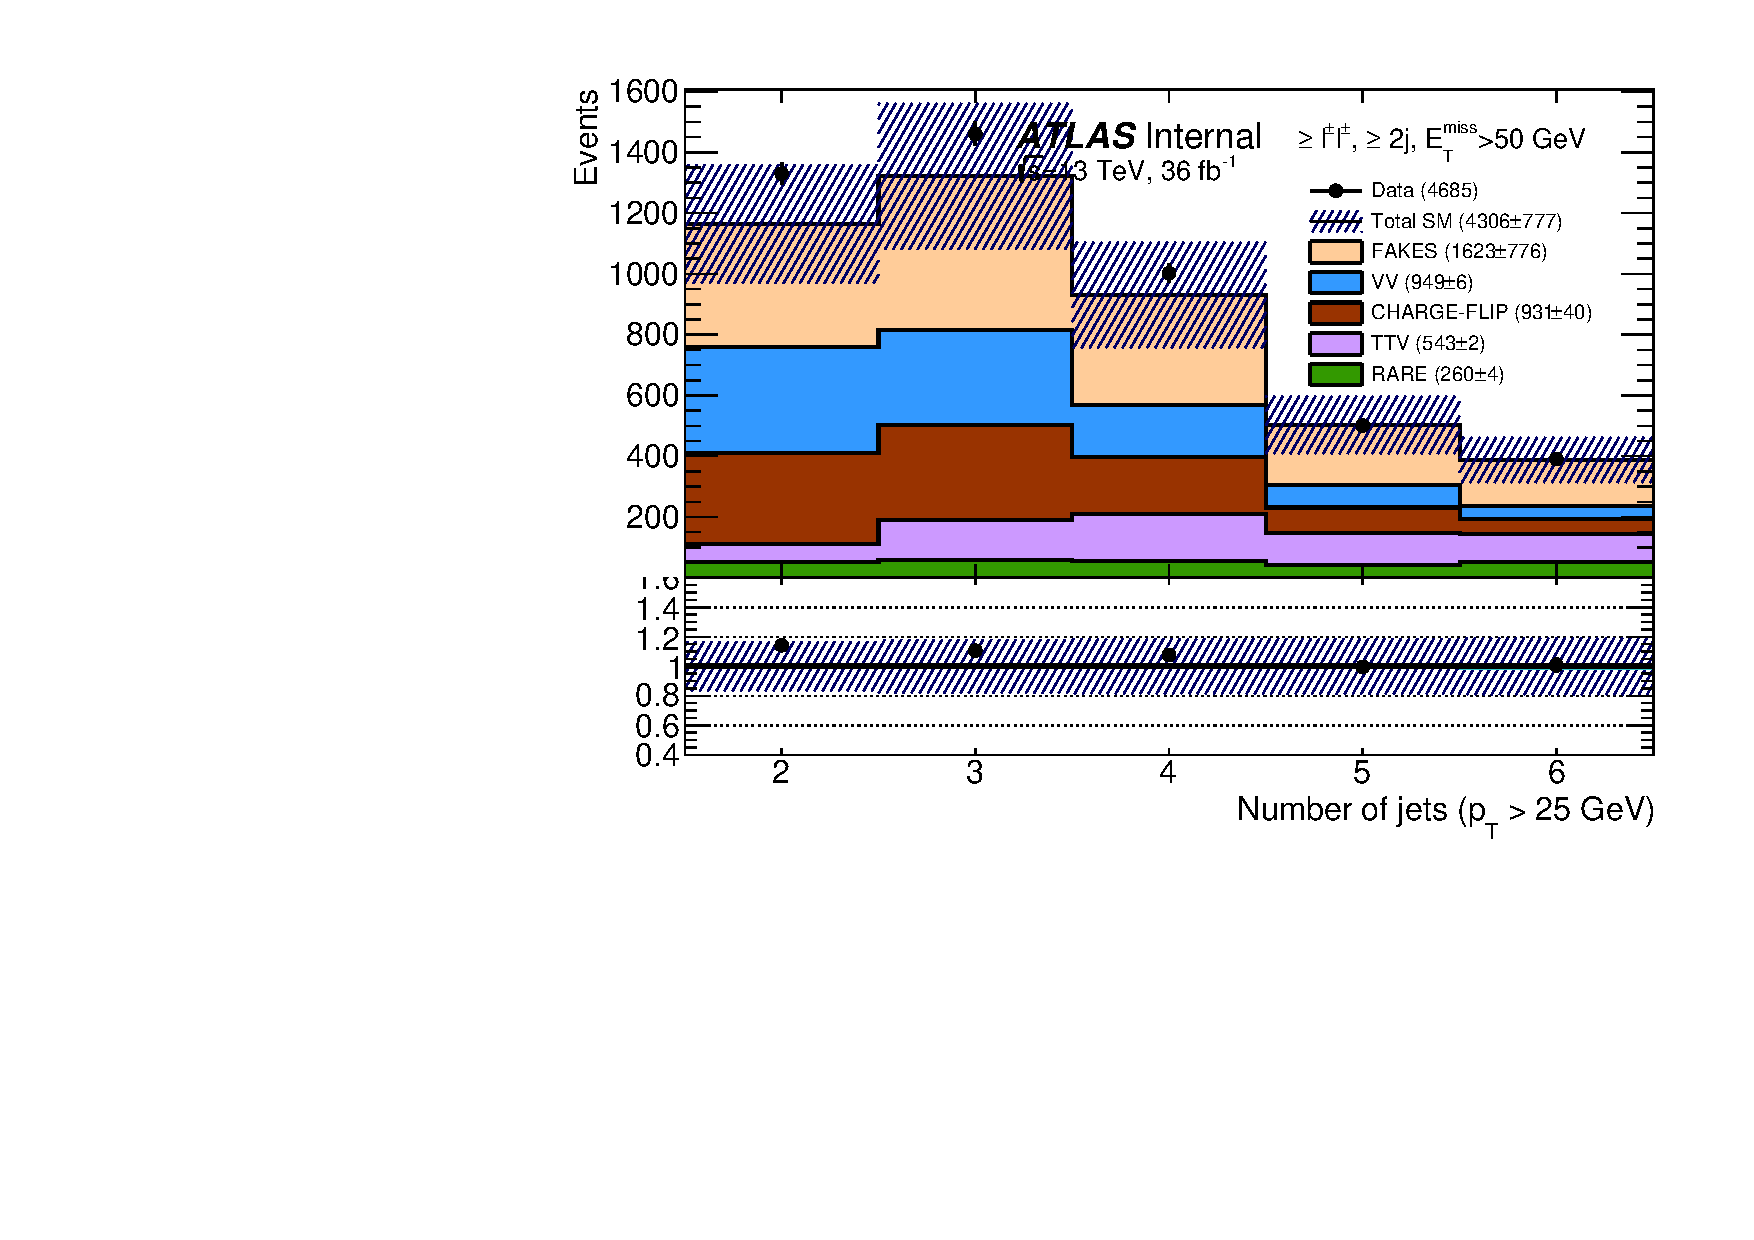
\includegraphics[width=\textwidth]{DILEP_2JMET50_njets25}\caption{}\end{subfigure}
\begin{subfigure}[t]{0.49\textwidth}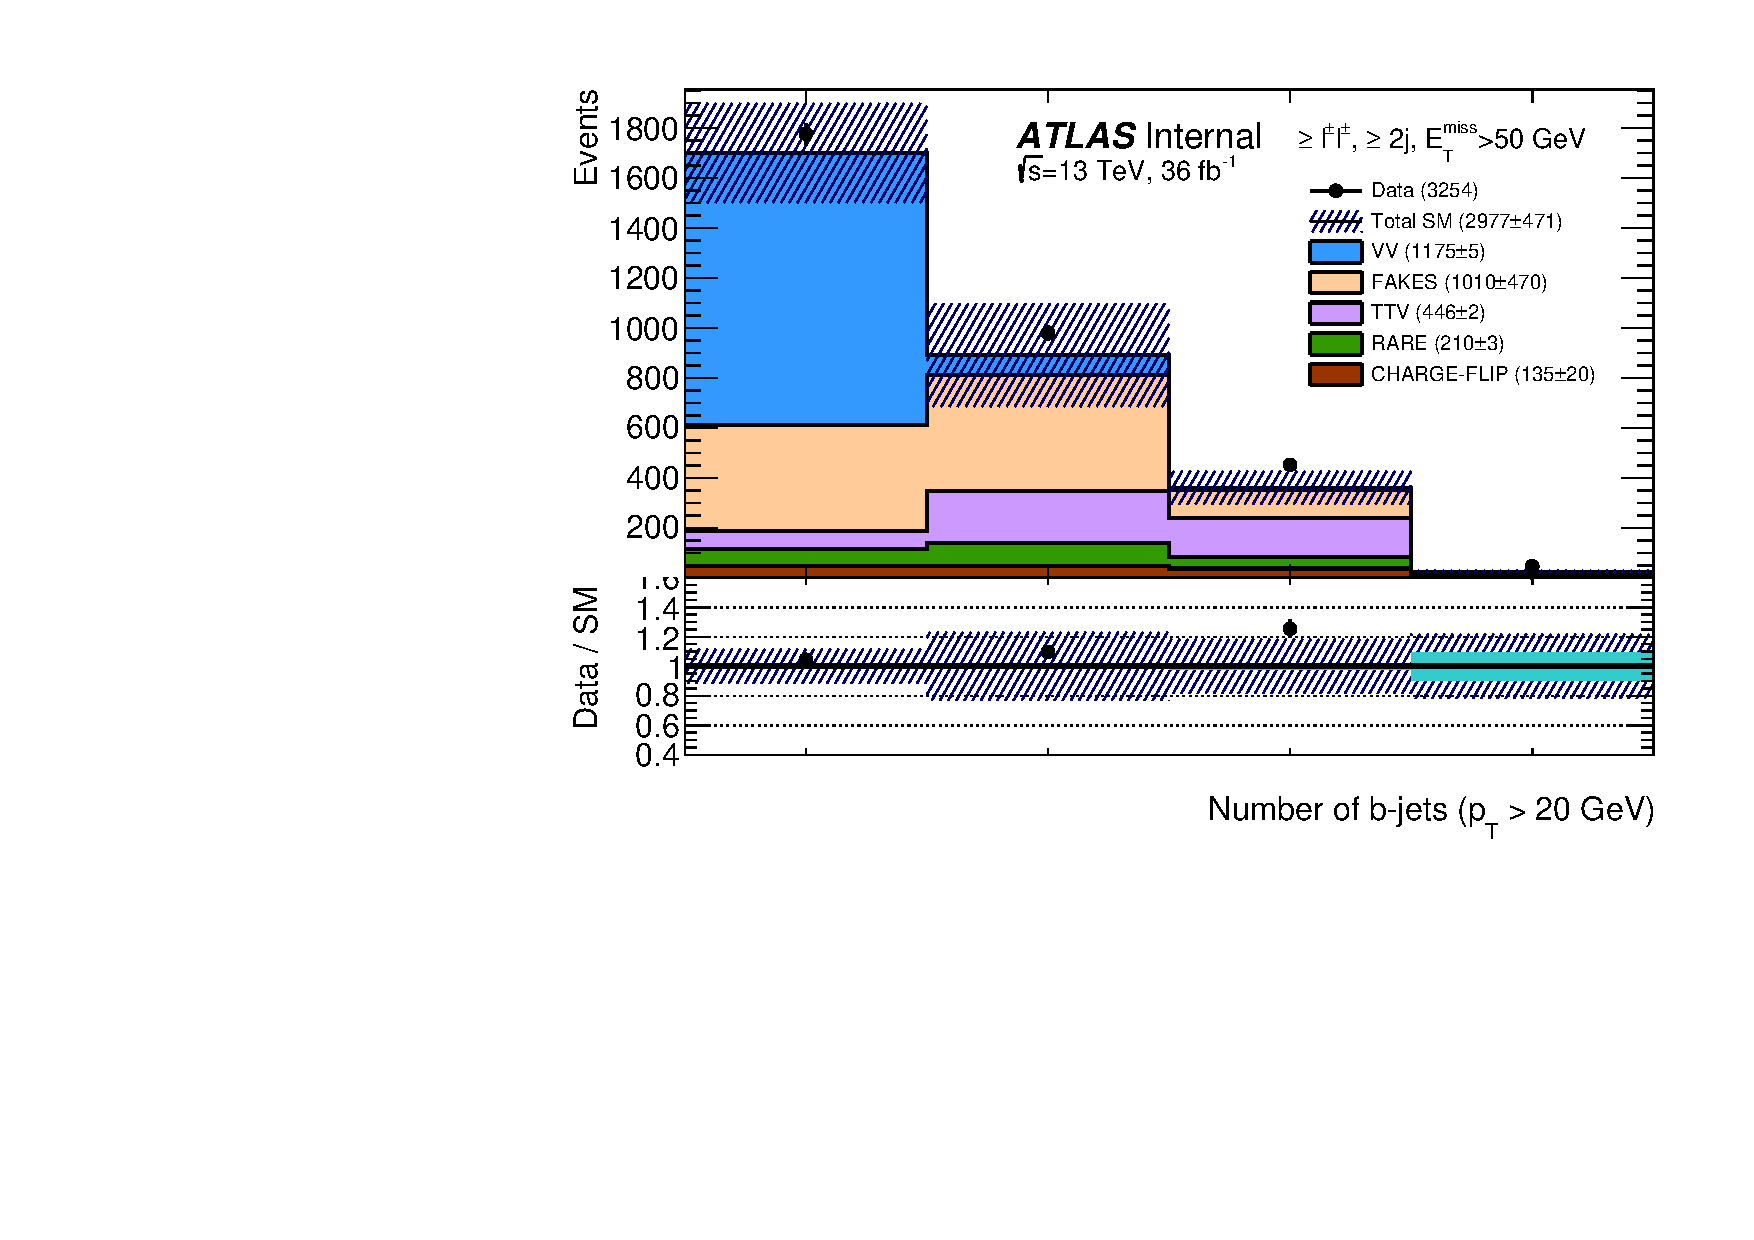
\includegraphics[width=\textwidth]{DILEP_2JMET50_nbjets}\caption{}\end{subfigure}
\begin{subfigure}[t]{0.49\textwidth}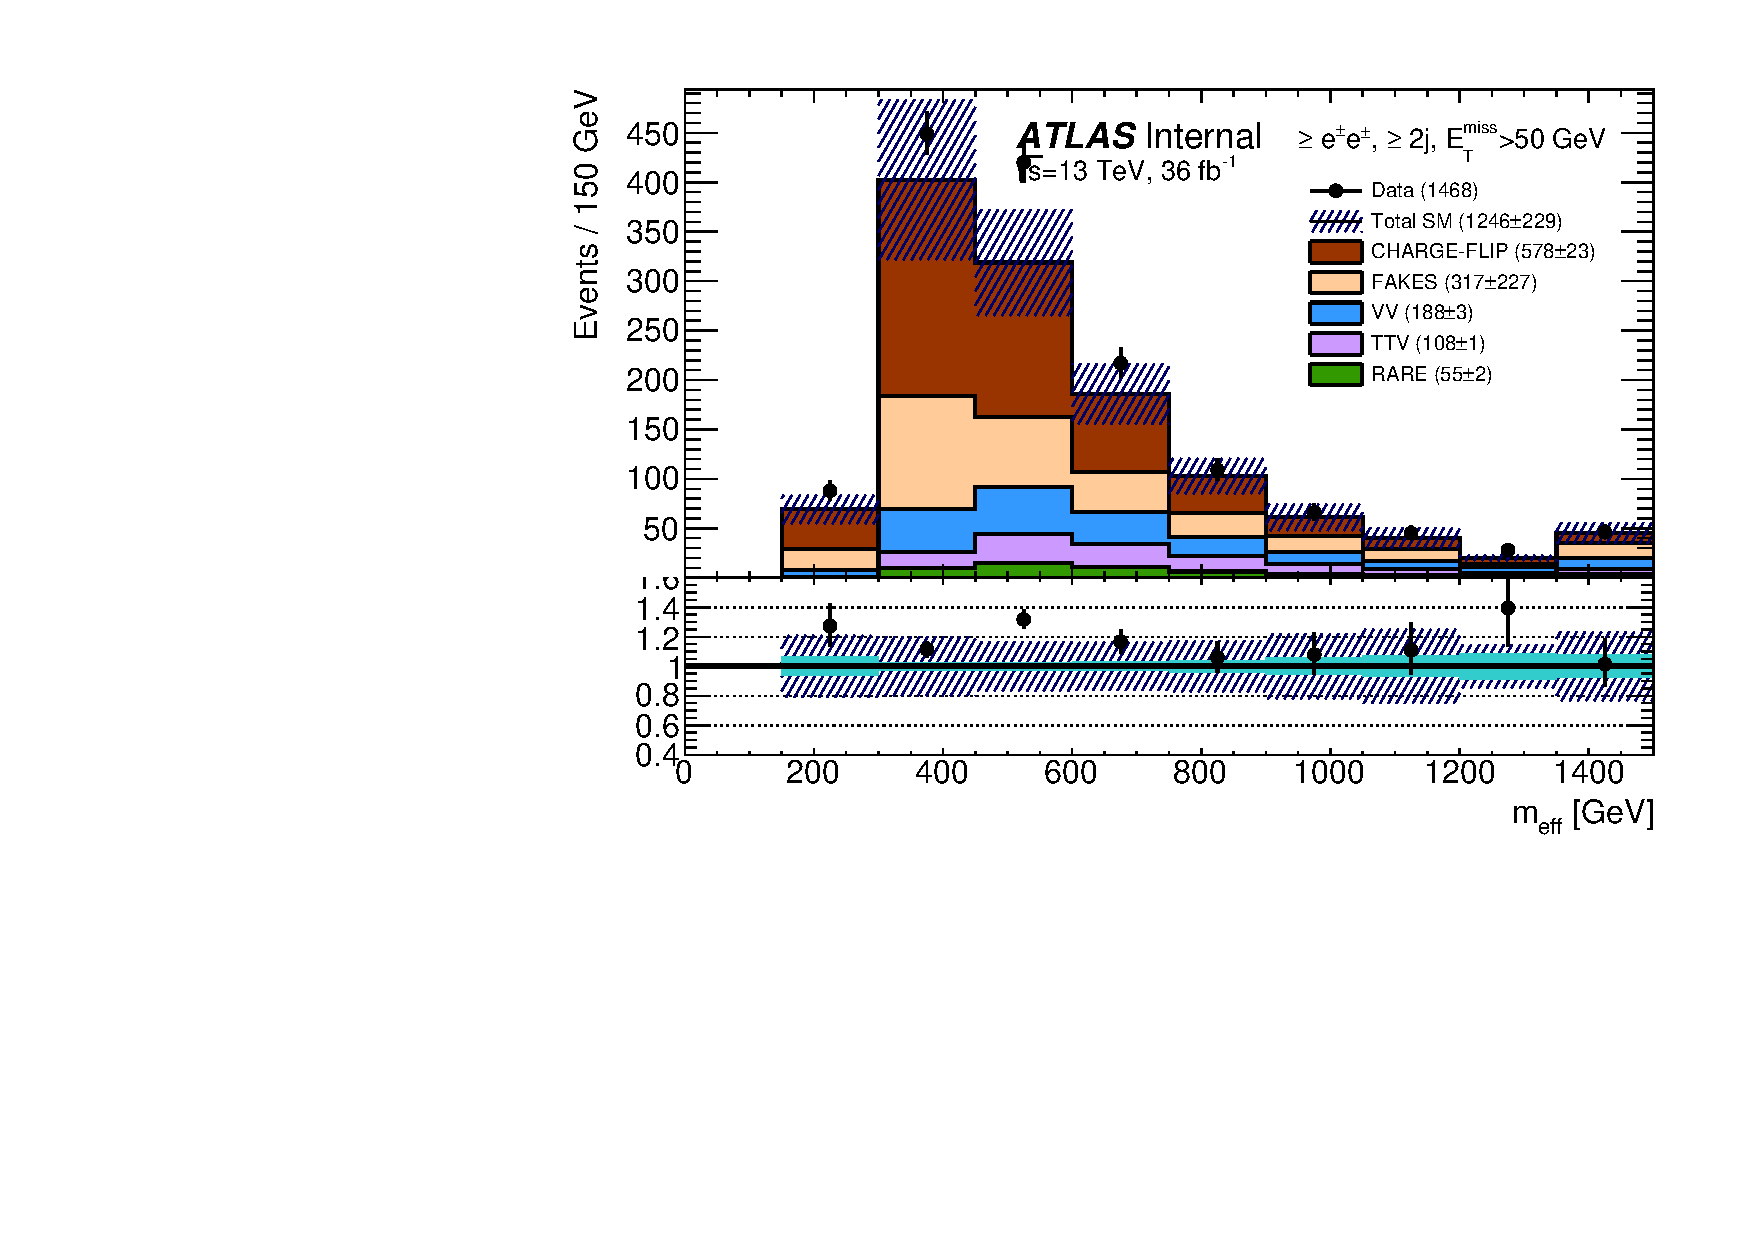
\includegraphics[width=\textwidth]{EE_2JMET50_meff}\caption{}\end{subfigure}
\begin{subfigure}[t]{0.49\textwidth}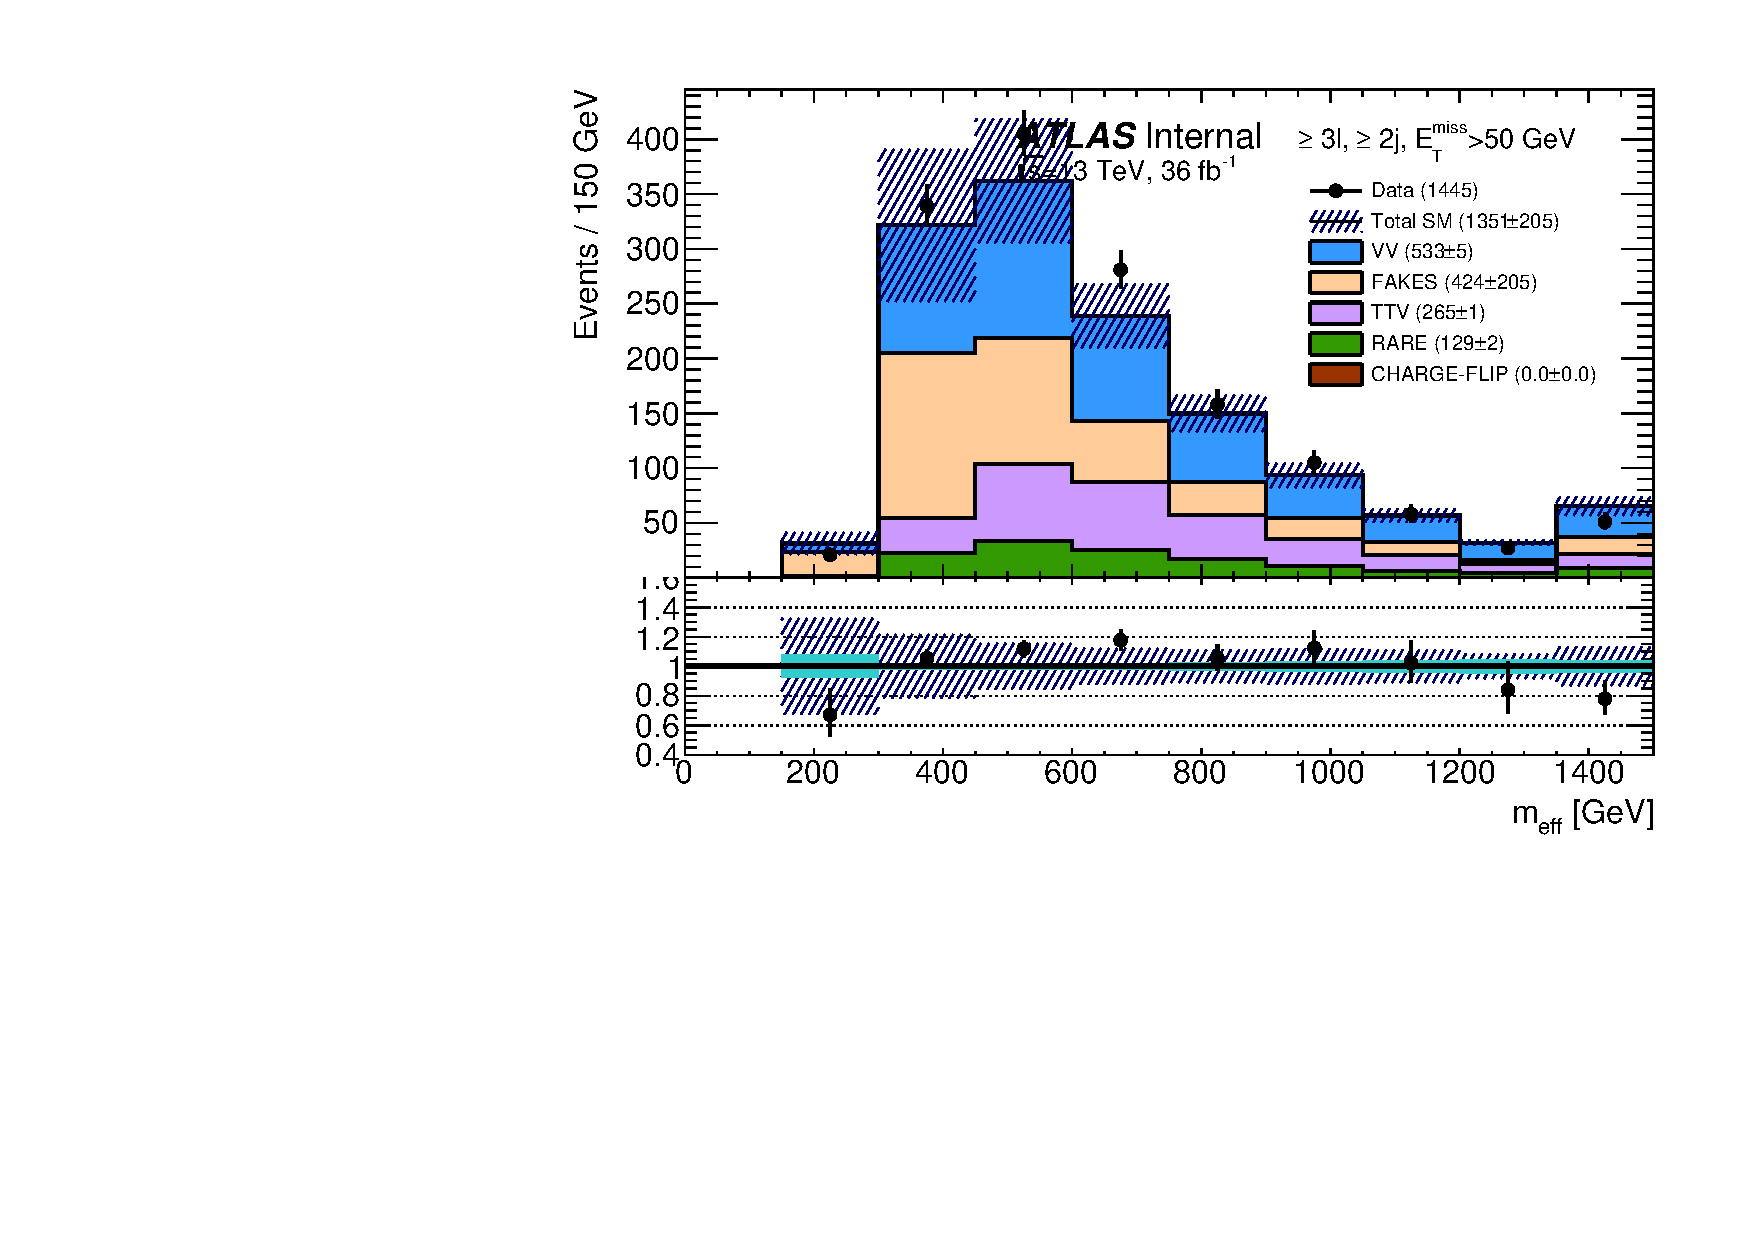
\includegraphics[width=\textwidth]{TRILEP_2JMET50_meff}\caption{}\end{subfigure}
\caption{
Distributions of the number of jets, of $b$-tagged jets and the effective mass after requiring at least two jets ($\pT>\SI{25}{GeV}$) and $\met>\SI{50}{GeV}$, 
as well as at least two same-sign leptons (a,b) or two same-sign electrons (c) or three leptons (d). 
The statistical uncertainties in the background prediction are included in the uncertainty band, 
as well as the full systematic uncertainties for backgrounds with fake or non-prompt leptons, or charge-flip. 
The light blue bands in the ratio plots show contributions from statistical uncertainties alone while the hashed area shows the total uncertainty.. 
The ``Rare'' category contains the contributions from associated production $\ttbar+WW/WZ$, 
as well as $t+Z/WZ/\ttbar$, $H+W/Z$, and triboson production. \textcolor{red}{[UPDATE: Remove numbers in the legend 
and move from upper case to lower case.]}
}
\label{fig:Bkg_distribs} 
\end{figure} 


\subsection{Validation of background estimates}
\label{sec:valid}

To check the validity and robustness of the background estimates, 
the distributions of several discriminating variables in data are compared 
with the predicted background after various requirements on the number of jets and $b$-jets. 
%Events are categorised based on the flavours of the selected leptons, and the different flavour channels are compared separately. 
Examples of such distributions are shown in Fig.~\ref{fig:Bkg_distribs}, 
and illustrate that the predictions and data agree fairly well. 

Dedicated validation regions are defined to test the estimate of the $\ttbar V$, $WZ$ and $W^\pm W^\pm$ SM processes contributing to the signal regions. The corresponding selections are summarized in Table~\ref{tab:VRdef}. 
In these regions, the overlap with the signal regions is resolved by vetoing events that contribute to the signal regions.  
%To further reduce contributions from electron charge mis-identification,  events are also vetoed in VR-$\ttbar W$ and VR-$W^\pm W^{\pm}jj$ if one of the two leading leptons is an electron with $|\eta|>1.37$\textcolor{red}{[UPDATE:Still true]}, since contributions from charge-flip electrons are smaller in the central region due to the lower amount of detector material in front of the calorimeters. 
The purity of the targeted processes in these regions ranges from about \textcolor{red}{[UPDATE:20\% to $50\%$]}. 

The observed yields in these validation regions, compared with the background predictions and uncertainties, 
can be seen in Table~\ref{tab:VR_yields}.
%, and the effective mass distributions are shown in Fig.~\ref{fig:VRd}--\ref{fig:VRf}.
There is good agreement between data and the estimated background for the validation regions.

\begin{table}[t!]
\hspace{0.5cm}
\def\arraystretch{1.1}
\centering
\resizebox{\textwidth}{!}
{\small
\begin{tabular}{|c|c|c|c|c|c|c|l|}
\hline    
Validation        &  $N_{\rm{lepton}}^{\rm{signal}}$ ($N_{\rm{lepton}}^{\rm{cand}}$)   & $N_{b\rm{-jets}}$  &  $N_{\rm{jets}}$  & $p^{}_{\rm{T,jet}}$  & \met\ & \meff\  & Other \\
Region Name       &  &  &  & [GeV]  & [GeV] & [GeV]  & \\
\hline\hline
$W^{\pm} W^{\pm}jj$ & $=2$ ($=2$)    &  $=0$ & $\geq 2$ &   $>50$ & $> 55$  & $> 650$ & veto $81<\mee<101$~GeV  \\
               	  & $=1$ SS pair  &	  &	     &         &   	&	  & $\pt^{\ell_2}>30$~GeV \\
               	  &		  &	  &	     &         &   	&	  & min$\left\{\Delta R(\ell_{1,2},j)\right\}>0.7$ \\
               	  &		  &	  &	     &         &   	&	  & min$\left\{\Delta R(\ell_1, \ell_2)\right\}>1.3$ \\
\hline
$WZ$4j            & $=3$ ($=3$)    &  $=0$ & $\geq 4$ &  $>25$   & --    & $> 450$ & $\met/\sum p_T^{\ell} < 0.7$ \\
\hline
$WZ$5j            & $=3$ ($=3$)    &  $=0$ & $\geq 5$ &  $>25$   & --    & $> 450$ & $\met/\sum p_T^{\ell} < 0.7$  \\ 
\hline
$\ttbar W$   	&$=2$ ($=2$)    &$\geq 1$   & $\geq 4$ ($e^\pm e^\pm$, $e^\pm \mu^\pm$) & $>40$ & $> 45$  & $> 550$   & $\pt(\ell_2)>40$~GeV\\
              	& $=1$ SS pair  &       &  $\geq 3$ ($\mu^\pm \mu^\pm$)   &  $>25$ &      &          & $\sum p_T^{b-jet}/\sum p_T^{jet}>0.25$ \\ 
\hline
$\ttbar Z$    	&$\geq 3$ (-) & $\geq 1$ & $\geq 3$ &  $>35$ &  --    & $> 450$  & $81<m_\text{SFOS}<101$~GeV \\
                &$\geq 1$ SFOS pair&     &          &       &         &         &  \\
\hline
All VRs & \multicolumn{7}{c|}{Veto events belonging to any SR} \\
\hline
\end{tabular}
}
\caption{Summary of the event selection in the validation regions (VRs). 
Requirements are placed on the number of signal leptons ($N_{\rm{lept}}^{\rm{signal}}$) 
and candidate leptons ($N_{\rm{lept}}^{\rm{cand}}$), the number of jets ($N_{\rm{jets}}$) 
or the number of $b$-jets with $\pt>\SI{20}{GeV}$ ($N_{b\rm{-jets}}$). The two leading-\pt 
leptons are referred to as $\ell_{1,2}$ with decreasing \pt. Additional requirements are set 
on \met, \meff, the invariant mass of the two leading electrons $m_{ee}$, the presence of SS 
leptons or a pair of same-flavour opposite-sign leptons (SFOS) and its invariant mass $m_\text{SFOS}$. 
A minimum angular separation between the leptons and the jets ($\Delta R (\ell, j)$) and between the two 
leptons ($\Delta R (\ell_{1}, \ell_2)$) is imposed in $W^\pm W^\pm$ VR. For the two $WZ$ VRs an upper cut 
on the ratio between the \met in the event and the sum of all selected leptons \pt (\met/$\sum{p_T^\ell}$) is required. 
An upper cut on the ratio between the sum of the \pt of all $b$-jets and that of all jets in the event ($\sum p_T^{b-j} / \sum{p_T^{j}}$) is 
considered only in the $\ttbar W$ VR.
}
\label{tab:VRdef}
\end{table}

\begin{table}[t!]
\hspace{0.5cm}
\def\arraystretch{1.1}
\centering
%\resizebox{\textwidth}{!}
%{\small
\begin{tabular}{|l|c|c|c|c|c|}
\hline    
 Validation Regions       & $WZ$4j & $WZ$5j  & $W^\pm W^{\pm}jj$& $\ttbar W$   & $\ttbar Z$  \\
\hline\hline
$t\bar{t}Z/\gamma^*$     & $  \pm  $ & $  \pm  $      & $  \pm  $  & $  \pm  $    & $  \pm  $  \\
$t\bar{t}W$              & $  \pm $  & $  \pm  $      & $  \pm  $  & $  \pm  $    & $  \pm  $  \\
$t\bar{t}H$              & $  \pm $  & $  \pm  $      & $  \pm  $  & $  \pm  $    & $  \pm  $  \\
$t\bar{t}t\bar{t}$       & $  \pm $  & $  \pm  $      & $  \pm  $  & $  \pm  $    & $  \pm  $  \\
$WW$                     & $  \pm $  & $  \pm  $      & $  \pm  $  & $  \pm  $    & $  \pm  $  \\
$WZ$                     & $  \pm $  & $  \pm  $      & $  \pm  $  & $  \pm  $    & $  \pm  $  \\
$ZZ$                     & $  \pm $  & $  \pm  $      & $  \pm  $  & $  \pm  $    & $  \pm  $  \\
Rare                     & $  \pm  $ & $  \pm  $      & $  \pm  $  & $  \pm  $    & $  \pm  $  \\
Fake/non-prompt leptons  & $  \pm  $ & $  \pm  $      & $  \pm  $  & $  \pm  $    & $  \pm $  \\
Charge-flip              & $-$       & $  \pm  $      & $  \pm  $  & $  \pm  $    & $-$  \\
\hline
Total SM  background   	& $-$        & $  \pm  $      & $  \pm  $  & $  \pm  $    & $-$  \\
\hline
Observed	   	& $-$        & $  \pm  $      & $  \pm  $  & $  \pm  $    & $-$  \\
\hline
\end{tabular}
%}
\caption{The numbers of observed data and expected background events in the validation regions. 
The ``Rare'' category contains the contributions from associated production $\ttbar+WW/WZ$, 
as well as $t+Z/WZ/\ttbar$, $H+W/Z$, and triboson production. Background categories shown as a ``$-$'' 
denote that they cannot contribute to a given region (e.g. charge flips in 3-lepton regions). 
The displayed yields include all sources of statistical and systematic uncertainties, 
except for the theoretical uncertainties which only affect the inclusive production cross-sections.}
\label{tab:VR_yields}
\end{table}

\section{Systematic uncertainties on the background estimation}
\label{sec:syst}

Figure~\ref{fig:PlotSR} summarises the contributions of the different sources of systematic uncertainty 
on the total SM background predictions in the signal regions.

The systematic uncertainties related to the same-sign prompt leptons background estimation 
arise from the accuracy of the theoretical and experimental modelling in the MC simulation.
The primary sources of systematic uncertainties are related to the jet energy scale calibration, 
jet energy resolution, $b$-tagging efficiency, and MC modelling and theoretical cross-section uncertainties. 
The statistical uncertainty of the simulated event samples is also taken into account.

The cross-sections used to normalise the MC samples are varied according to the uncertainty in the 
cross-section calculation, that is, 13\% for $\ttbar W$, 12\% for $\ttbar Z$ production~\cite{YR4}, 6\% for diboson
production~\cite{pubnote_mc_multiboson}, 8\% for $\ttbar H$~\cite{YR4} and 30\% for $\ttbar\ttbar$~\cite{Alwall:2014hca}. 
Additional uncertainties are assigned to some of these backgrounds to account for the theoritical modelling of the kinematic 
distributions in the MC simulation. For $\ttbar W$ and $\ttbar Z$, the predictions from the \AMCATNLO and \SHERPA generators are compared, 
and the renormalisation and factorisation scales used to generate these samples are varied, 
leading to a $\sim$\textcolor{red}{[UPDATE:30\%]} uncertainty on the expected SR yields for these processes. 
For dibosons, uncertainties are estimated by varying the renormalisation, factorisation and resummation scales, 
leading to a $\sim$\textcolor{red}{[UPDATE:40-50\%]} uncertainty for these processes after the SR selections. 
For $\ttbar H$, $\ttbar \ttbar$ and Rare production processes, a conservative 50\% uncertainty 
on their total contribution is assigned. 

Uncertainties in the FNP lepton background estimate are assigned due to the limited number 
of data events in the loose and tight lepton control regions.
In addition, systematic uncertainties of \textcolor{red}{[UPDATE:50-60\%]} are assigned to the FNP fake rate to account 
for potentially different 
compositions (heavy flavour, light flavour or conversions) between the regions used to measure these probabilities and the SRs, 
as well as the contamination from prompt leptons in the former regions. Similarly a \textcolor{red}{[UPDATE:5\%]} systematic is assigned to 
$\epsilon$ determination. This leads to overall FNP background uncertainties in the total background estimates 
of \textcolor{red}{[UPDATE:5--32\%]} depending on the signal region.

The uncertainty on the electron charge-flip probability mainly originates from the limited number of events used in 
the charge-flip probability measurement regions and the uncertainty related to the background subtraction 
beyond the $Z$ peak. The relative error on the charge-flip is below \textcolor{red}{[UPDATE:20\%]} for lepton \pt above 20 GeV.

\begin{figure}[H]
\begin{center}
\begin{subfigure}[t]{0.95\textwidth}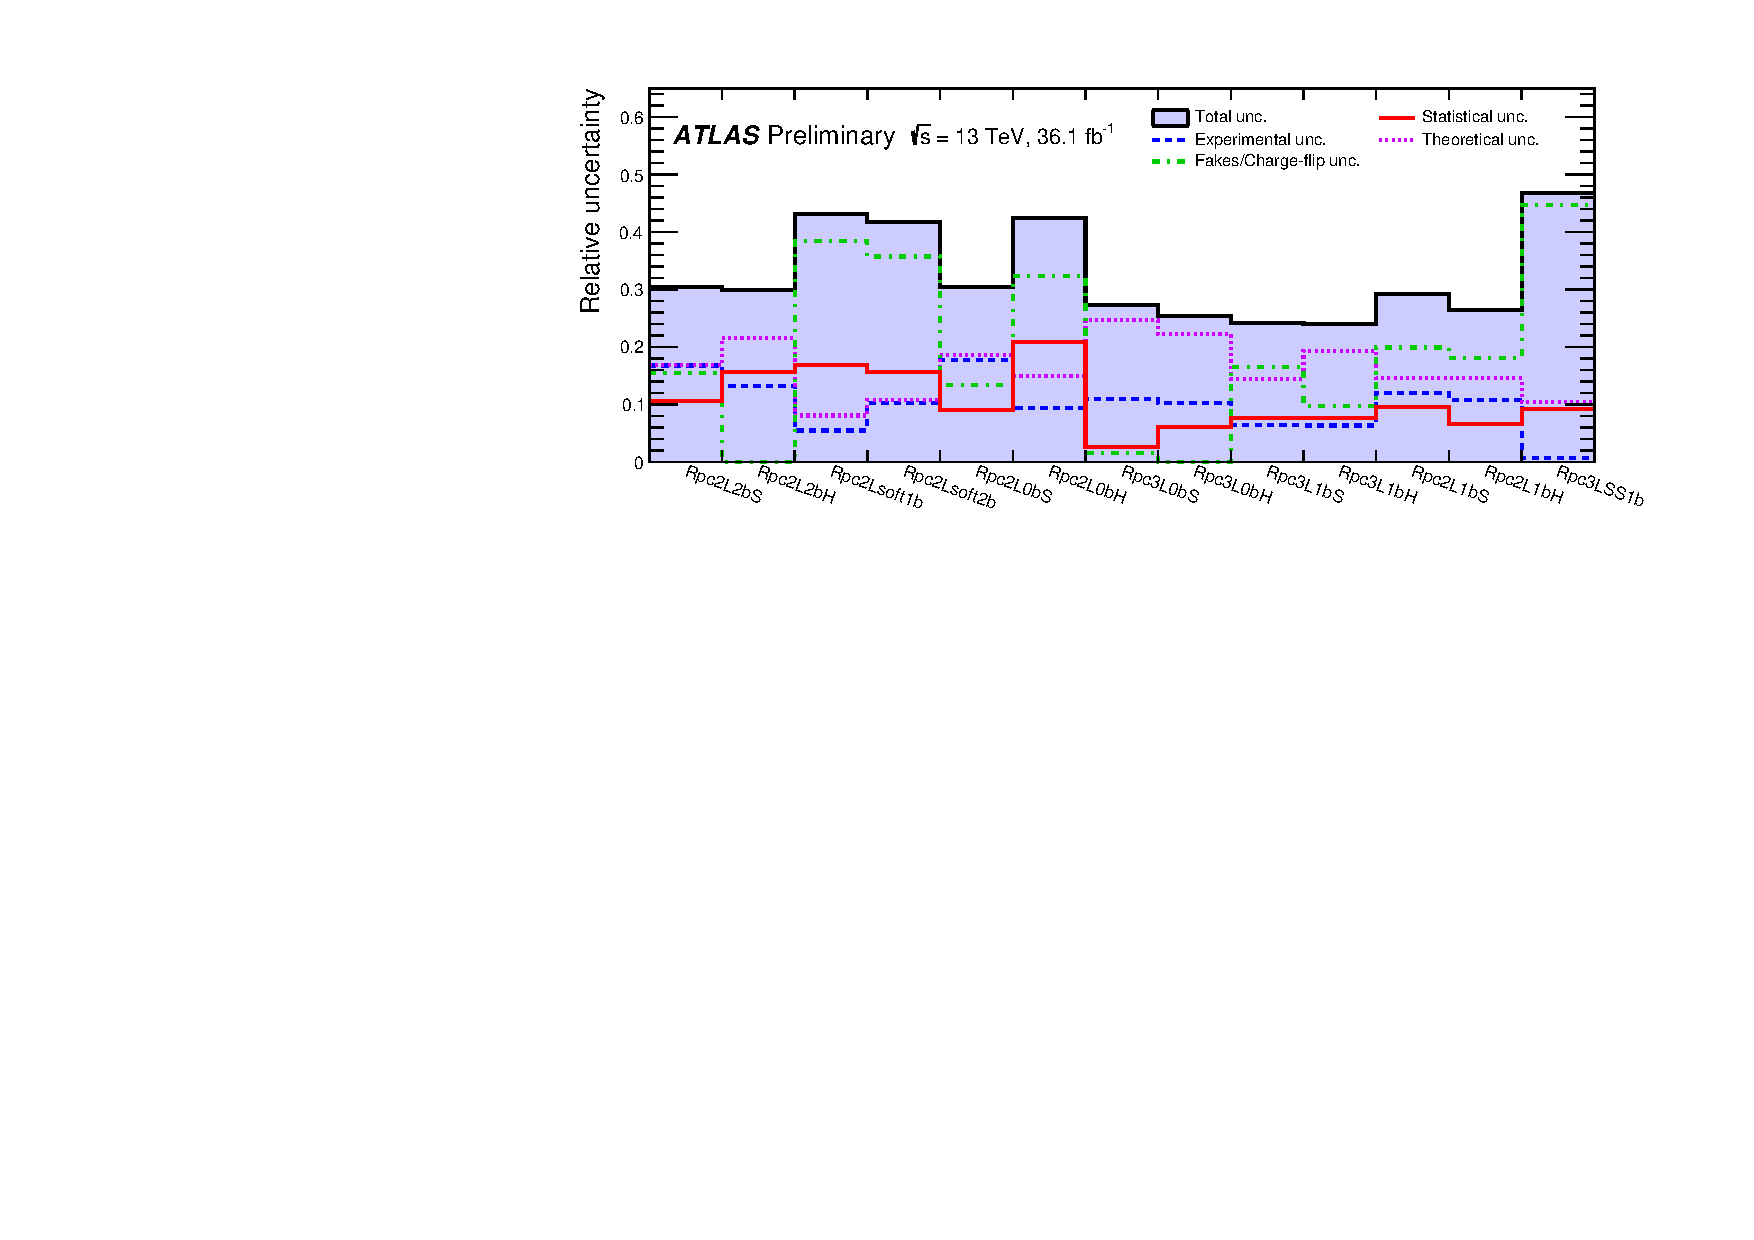
\includegraphics[width=\textwidth]{SystematicsSummary}\caption{}\end{subfigure} \\
\begin{subfigure}[t]{0.87\textwidth}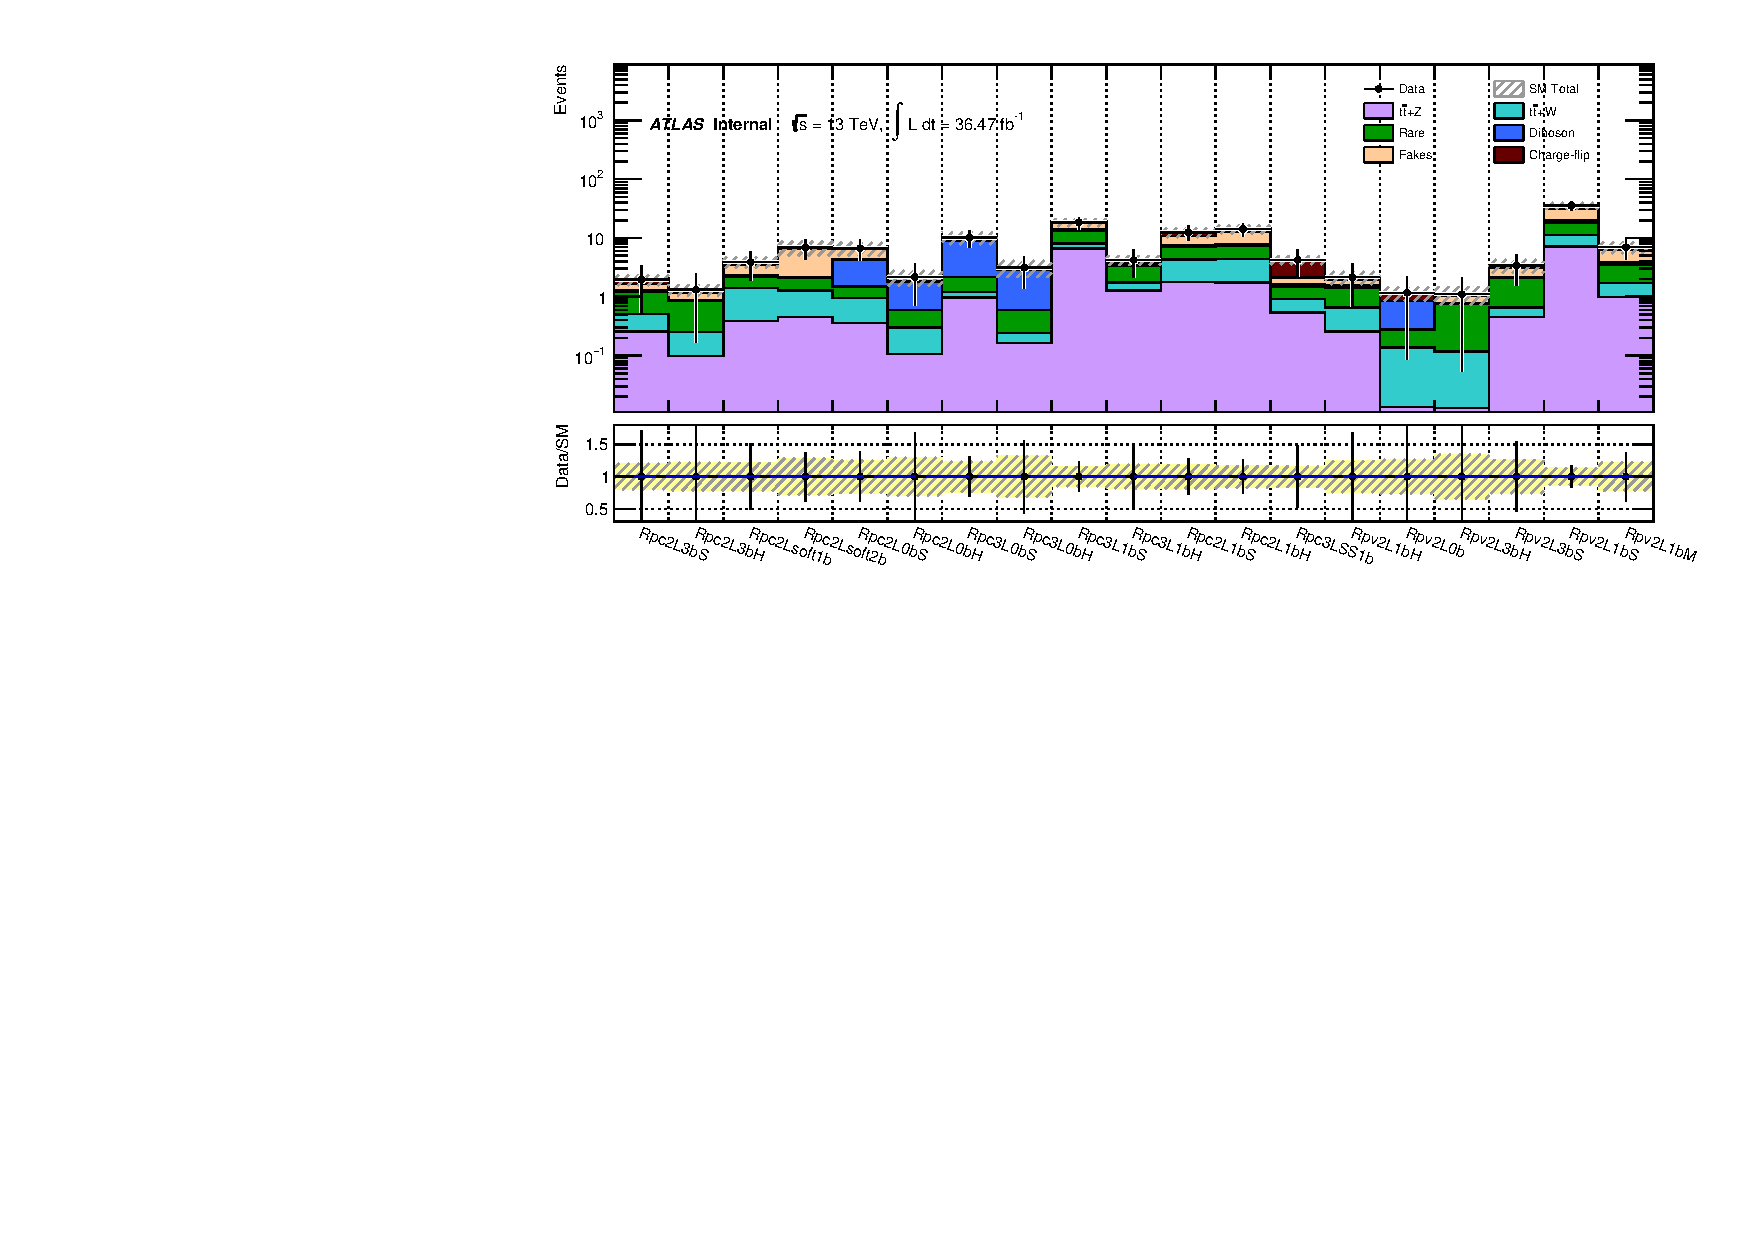
\includegraphics[width=\textwidth]{SRsummary}\caption{}\end{subfigure}
\end{center}
\caption{Relative systematic uncertainties and comparison of the observed and expected event yields in each signal region. 
The background expectations are those obtained from the background-only fits, presented in Table~\ref{tab:SR_yields}. 
\textcolor{red}{[UPDATE: Put all signal regions with final notations. Add ratio plot below SR Event Yields]}} 
\label{fig:PlotSR}
\end{figure}

%\begin{table}[h!]
%\begin{center}
%\caption{The main sources of systematic uncertainty on the SM background estimates for the four signal regions are shown 
%and their values given as relative uncertainties in the expected signal region background event yields. 
%The individual components can be correlated and therefore do not necessarily add up in quadrature to the total systematic uncertainty.
%For reference, the total number of expected background events is also shown.
%}
%\label{tab:SR_syst}
%{\small
%\begin{tabular}{lrrrr}
%\noalign{\smallskip}\hline\hline\noalign{\smallskip}
%         & SR0b3j         & SR0b5j     & SR1b & SR3b     \\[-0.05cm]
%\noalign{\smallskip}\hline\hline\noalign{\smallskip}
%Diboson theoretical uncertainties    & 23\%  &  16\%   &  1\%  &$<$1\%   \\
%$\ttbar V$ theoretical uncertainties & 3\%   &  4\%    & 13\%  &  9\%   \\
%Other theoretical uncertainties      & 5\%   &  3\%    &  9\%  & 15\%   \\
%\noalign{\smallskip}\hline\noalign{\smallskip}
%MC statistical uncertainties         & 11\%  &  14\%   &  3\%  &  6\%   \\
%\noalign{\smallskip}\hline\noalign{\smallskip}
%Jet energy scale        & 12\%   &  11\%  & 6\%    & 5\%   \\
%Jet energy resolution   & 3\%    &  9\%   & 2\%    & 3\%   \\
%$b$-tagging             & 4\%    &  6\%   & 3\%    & 10\%   \\
%PDF                     & 6\%    &  6\%   & 6\%    & 8\%   \\
%Fake/non-prompt leptons & 18\%    &  20\%   & 18\%   & 21\%   \\
%Charge flip             & --     & 1\% & 3\%    & 8\%   \\
%\noalign{\smallskip}\hline\noalign{\smallskip}
%Total background uncertainties & 30\%   & 34\%   & 22\%   & 31\%   \\
%\noalign{\smallskip}\hline\hline\noalign{\smallskip}
%Total background events & $1.5$ & $0.88$ & $4.5$ & $0.80$\\
%\noalign{\smallskip}\hline\hline\noalign{\smallskip}
%\end{tabular}
%}
%\end{center}
%\end{table}
	



%\section{Results}
%\label{sec:bkg}
%\begin{table}[htb!]
\begin{center}
\setlength{\tabcolsep}{0.0pc}
\caption{The number of observed data events and expected background contributions in the signal regions. 
The $p$-value of the observed events for the background-only hypothesis is denoted by $p(s = 0)$. 
The ``Rare'' category contains the contributions from associated production of $\ttbar$ with $h/WW/t/\ttbar$, 
as well as $tZ$, $Wh$, $Zh$, and triboson production. 
Background categories shown as ``$-$'' denote that they cannot contribute to a given region (charge flips or $W^\pm W^\pm jj$ in 3-lepton regions). 
The individual uncertainties can be correlated and therefore do not necessarily add up in quadrature to the total systematic uncertainty. 
}
\label{tab:SR_yields}
{\small
\begin{tabular*}{\textwidth}{@{\extracolsep{\fill}}lcccc}
\noalign{\smallskip}\hline\hline\noalign{\smallskip}
         & SR0b3j         & SR0b5j     & SR1b & SR3b     \\[-0.05cm]
\noalign{\smallskip}\hline\hline\noalign{\smallskip}
Observed events         & $3$     &  $3$  & $7$  & $1$            \\
\noalign{\smallskip}\hline\noalign{\smallskip}
Total background events & $1.5 \pm 0.4$ & $0.88 \pm 0.29$ & $4.5 \pm 1.0$ & $0.80 \pm 0.25$\\
$p(s = 0)$                &  0.13  &  0.04  &  0.15  &   0.36   \\
\noalign{\smallskip}\hline\noalign{\smallskip}
Fake/non-prompt leptons & $<0.2$ & $0.05\pm 0.18$ & $0.8 \pm 0.8$ & $0.13 \pm 0.17$\\
Charge-flip & $-$ & $0.02 \pm 0.01$ & $0.60 \pm 0.12$ & $0.19 \pm 0.06$\\
$t\bar{t}W$ & $0.02 \pm 0.01$ & $0.08 \pm 0.04$ & $1.1 \pm 0.4$ & $0.10 \pm 0.05$\\
$t\bar{t}Z$ & $0.10 \pm 0.04$ & $0.05 \pm 0.03$ & $0.92 \pm 0.31$ & $0.14 \pm 0.06$\\
$WZ$ & $1.2 \pm 0.4$ & $0.48 \pm 0.20$ & $0.18 \pm 0.11$ & $<0.02$\\
$W^\pm W^\pm jj$ & $-$ & $0.12 \pm 0.07$ & $0.03 \pm 0.02$ & $<0.01$\\
$ZZ$ & $<0.03$ & $<0.04$ & $<0.03$ & $<0.03$\\
Rare & $0.14 \pm 0.08$ & $0.07 \pm 0.05$ & $0.8 \pm 0.4$ & $0.24 \pm 0.14$\\  
\noalign{\smallskip}\hline\hline\noalign{\smallskip}
\end{tabular*}
}
\end{center}
\end{table}

\begin{figure}[t!]
\centering
\begin{subfigure}[t]{0.49\textwidth}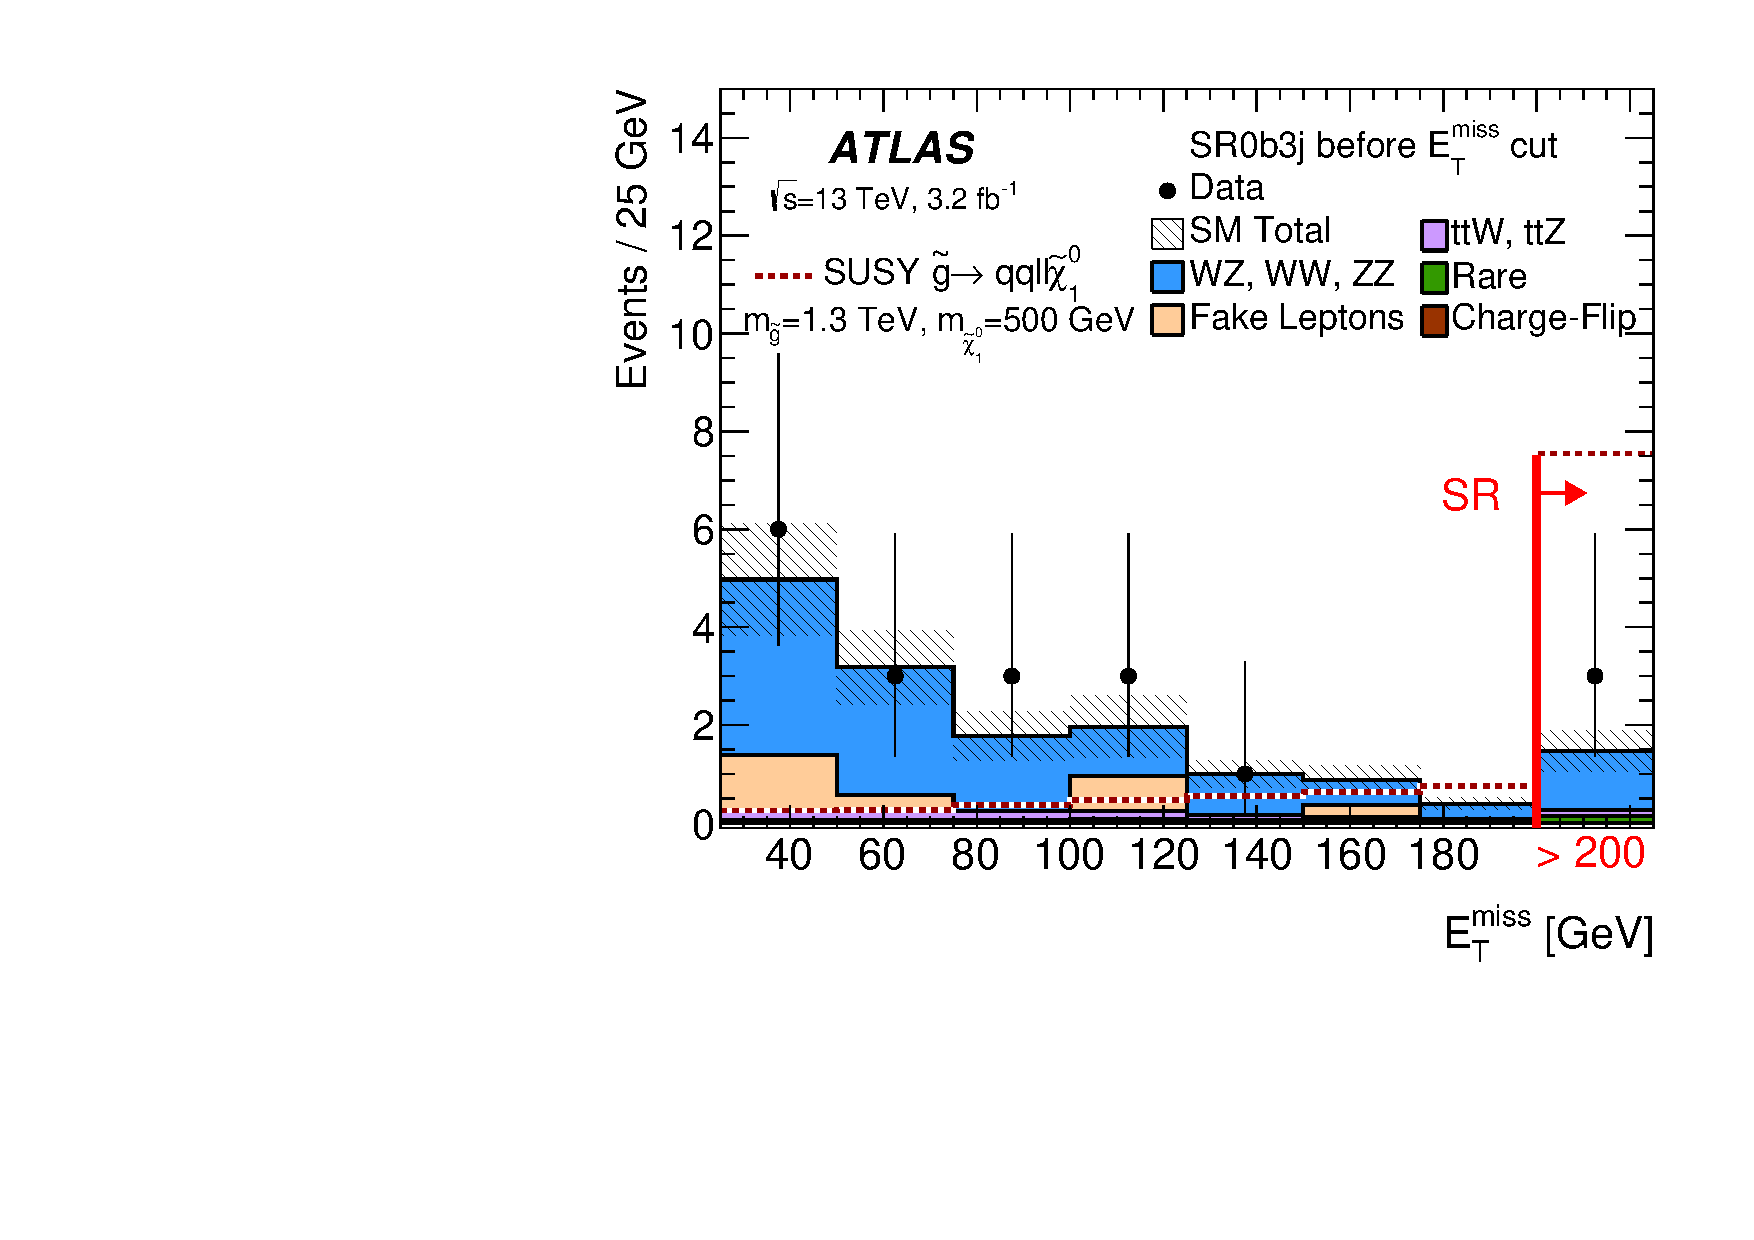
\includegraphics[width=\textwidth]{FIGURES/CONF_SR0b3j.pdf}
\caption{}\label{fig:Results_SR0b3j}\end{subfigure}
\begin{subfigure}[t]{0.49\textwidth}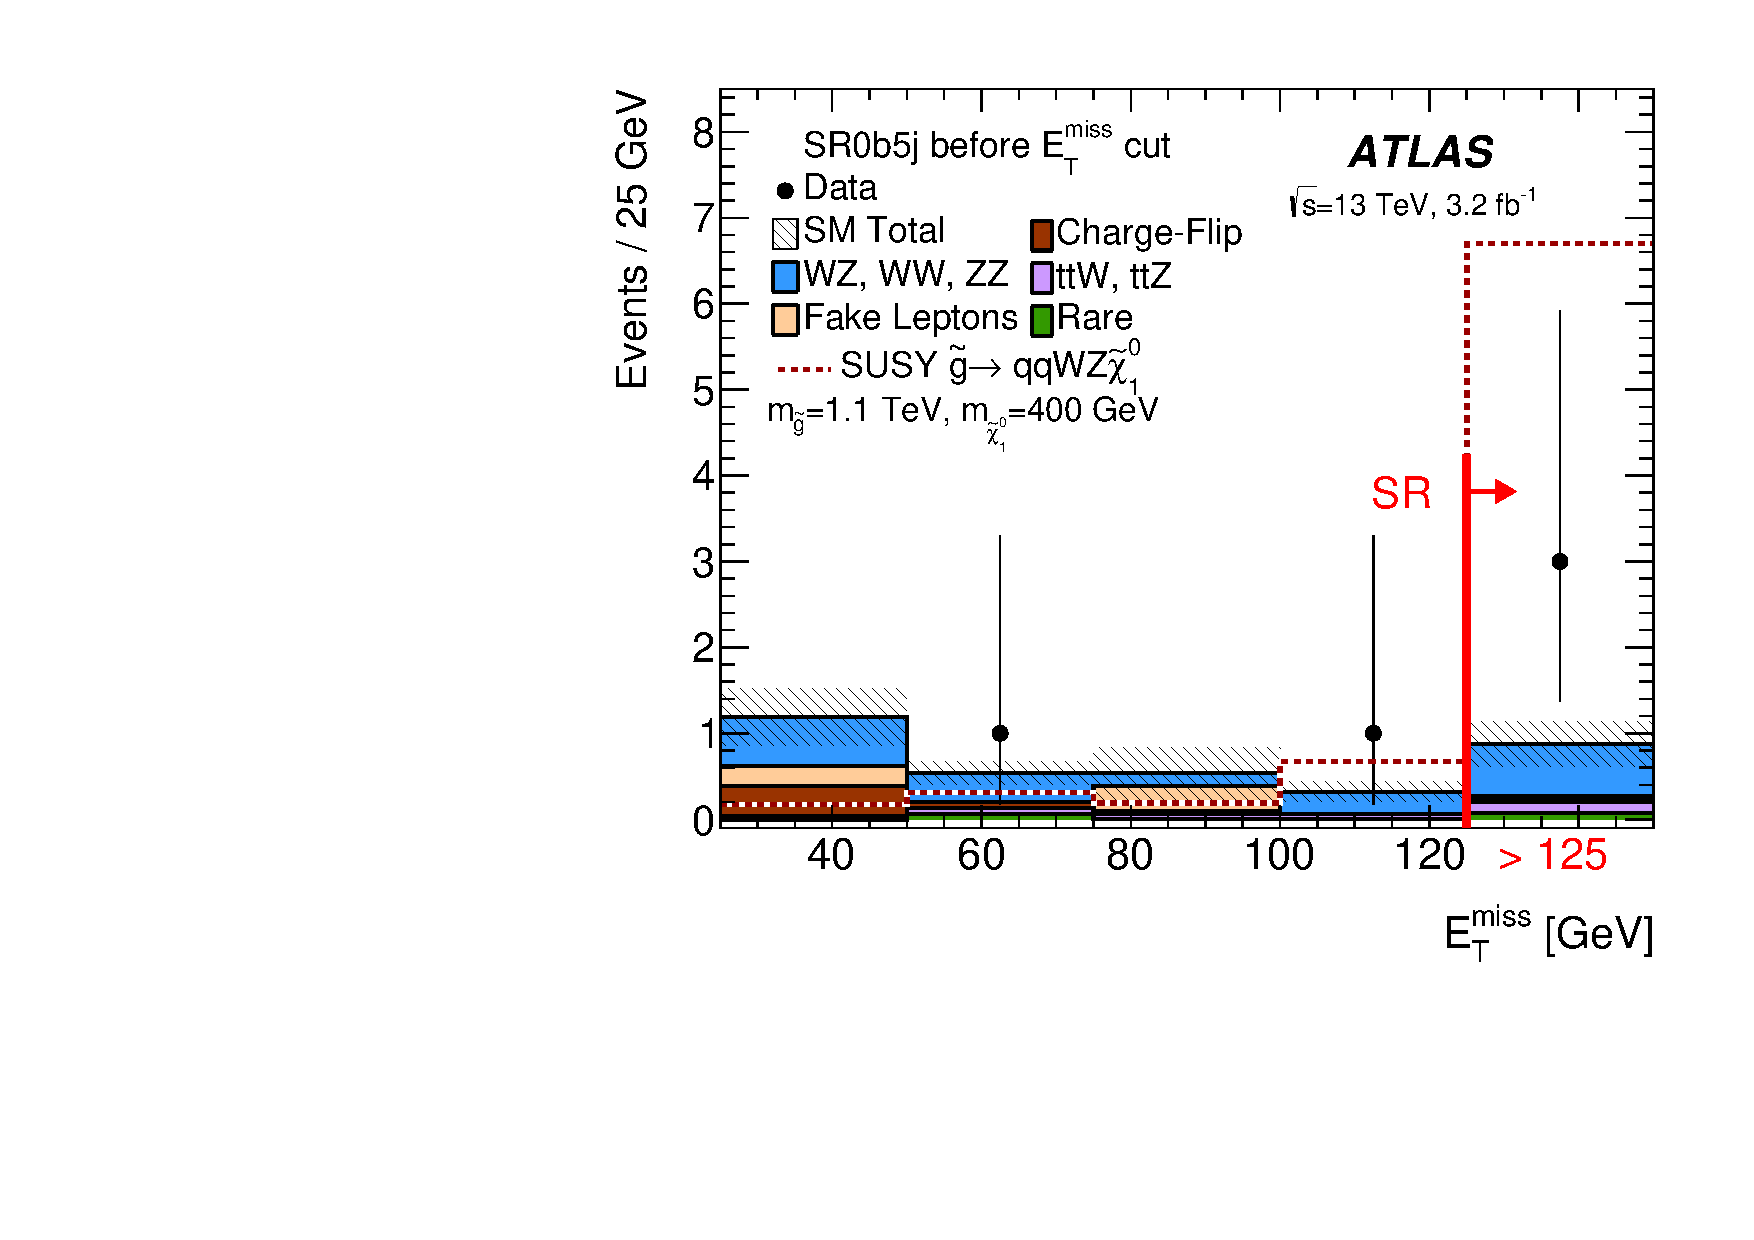
\includegraphics[width=\textwidth]{FIGURES/CONF_SR0b5j.pdf}
\caption{}\label{fig:Results_SR0b5j}\end{subfigure}
\begin{subfigure}[t]{0.49\textwidth}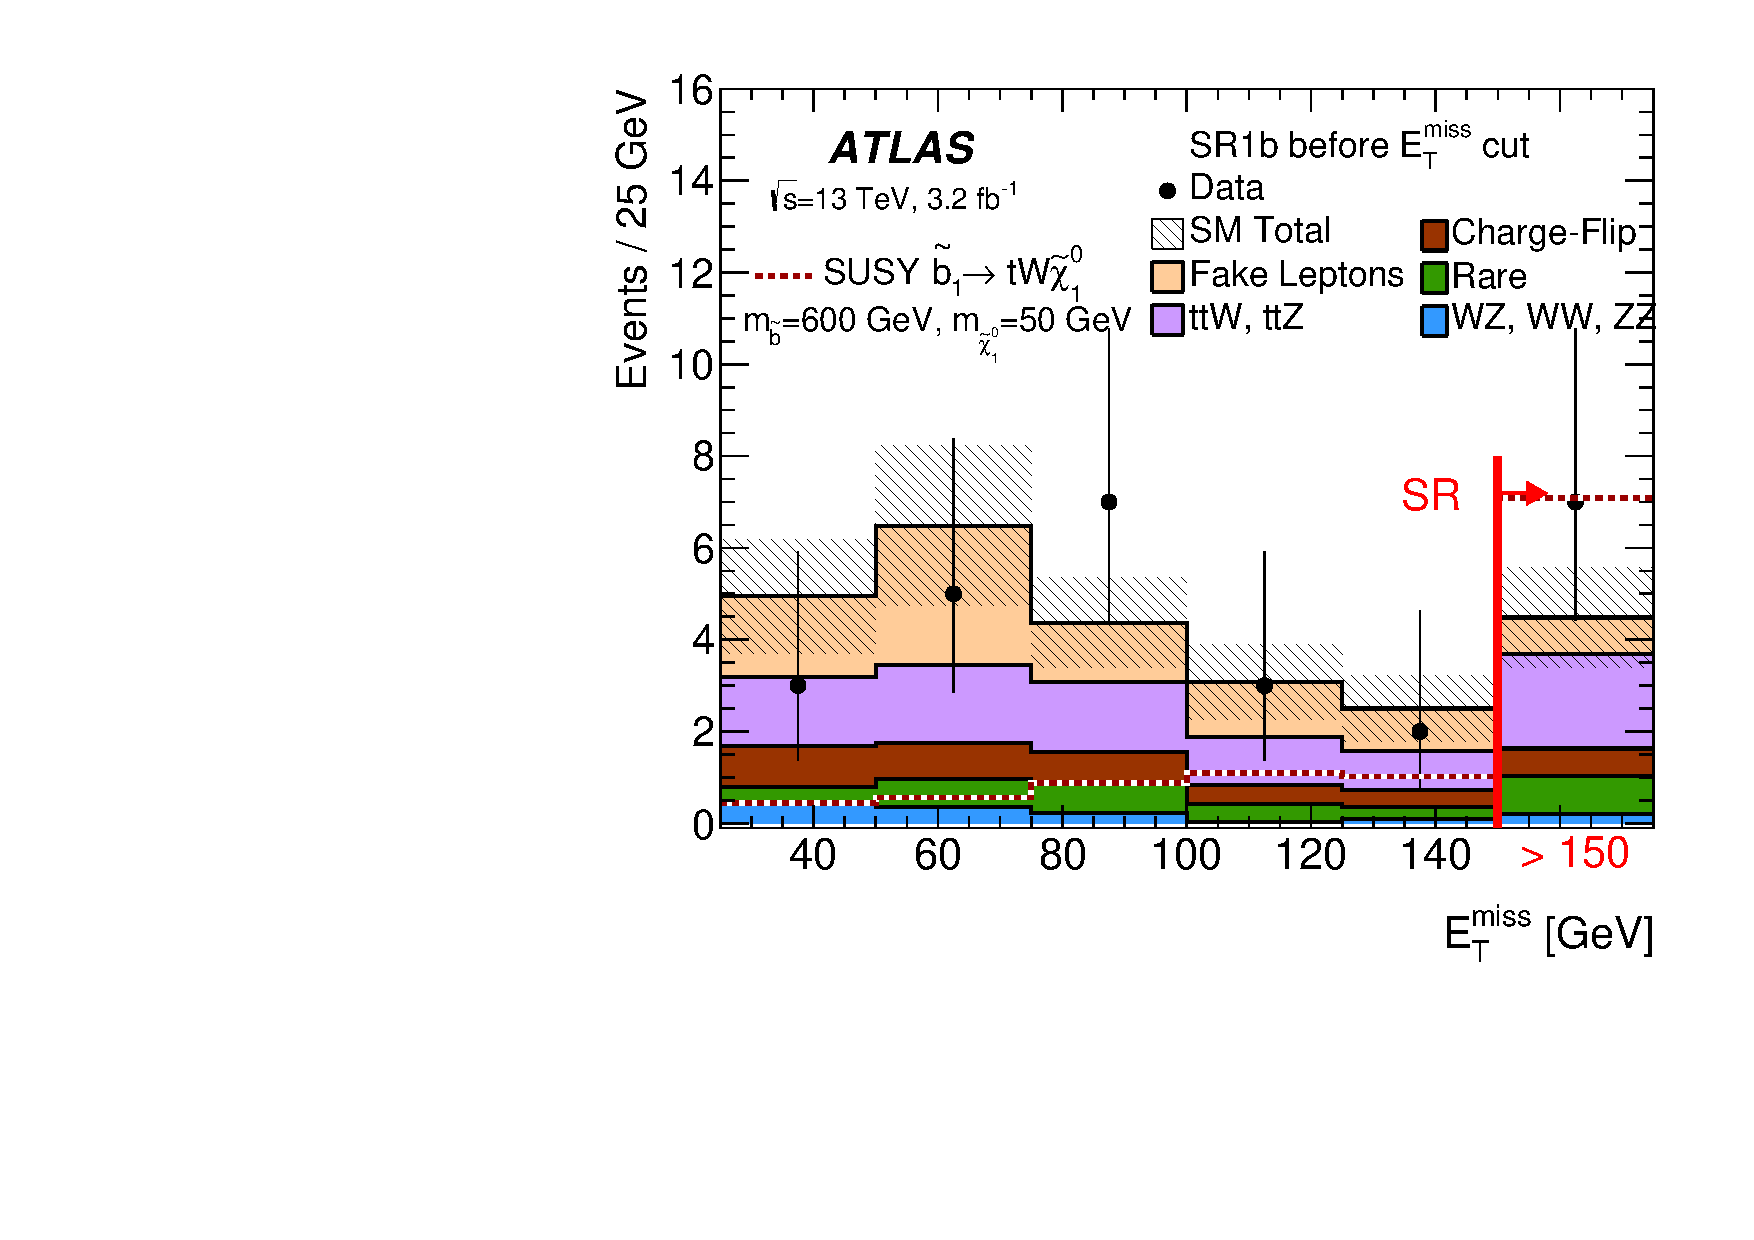
\includegraphics[width=\textwidth]{FIGURES/CONF_SR1b.pdf}
\caption{}\label{fig:Results_SR1b}\end{subfigure}
\begin{subfigure}[t]{0.49\textwidth}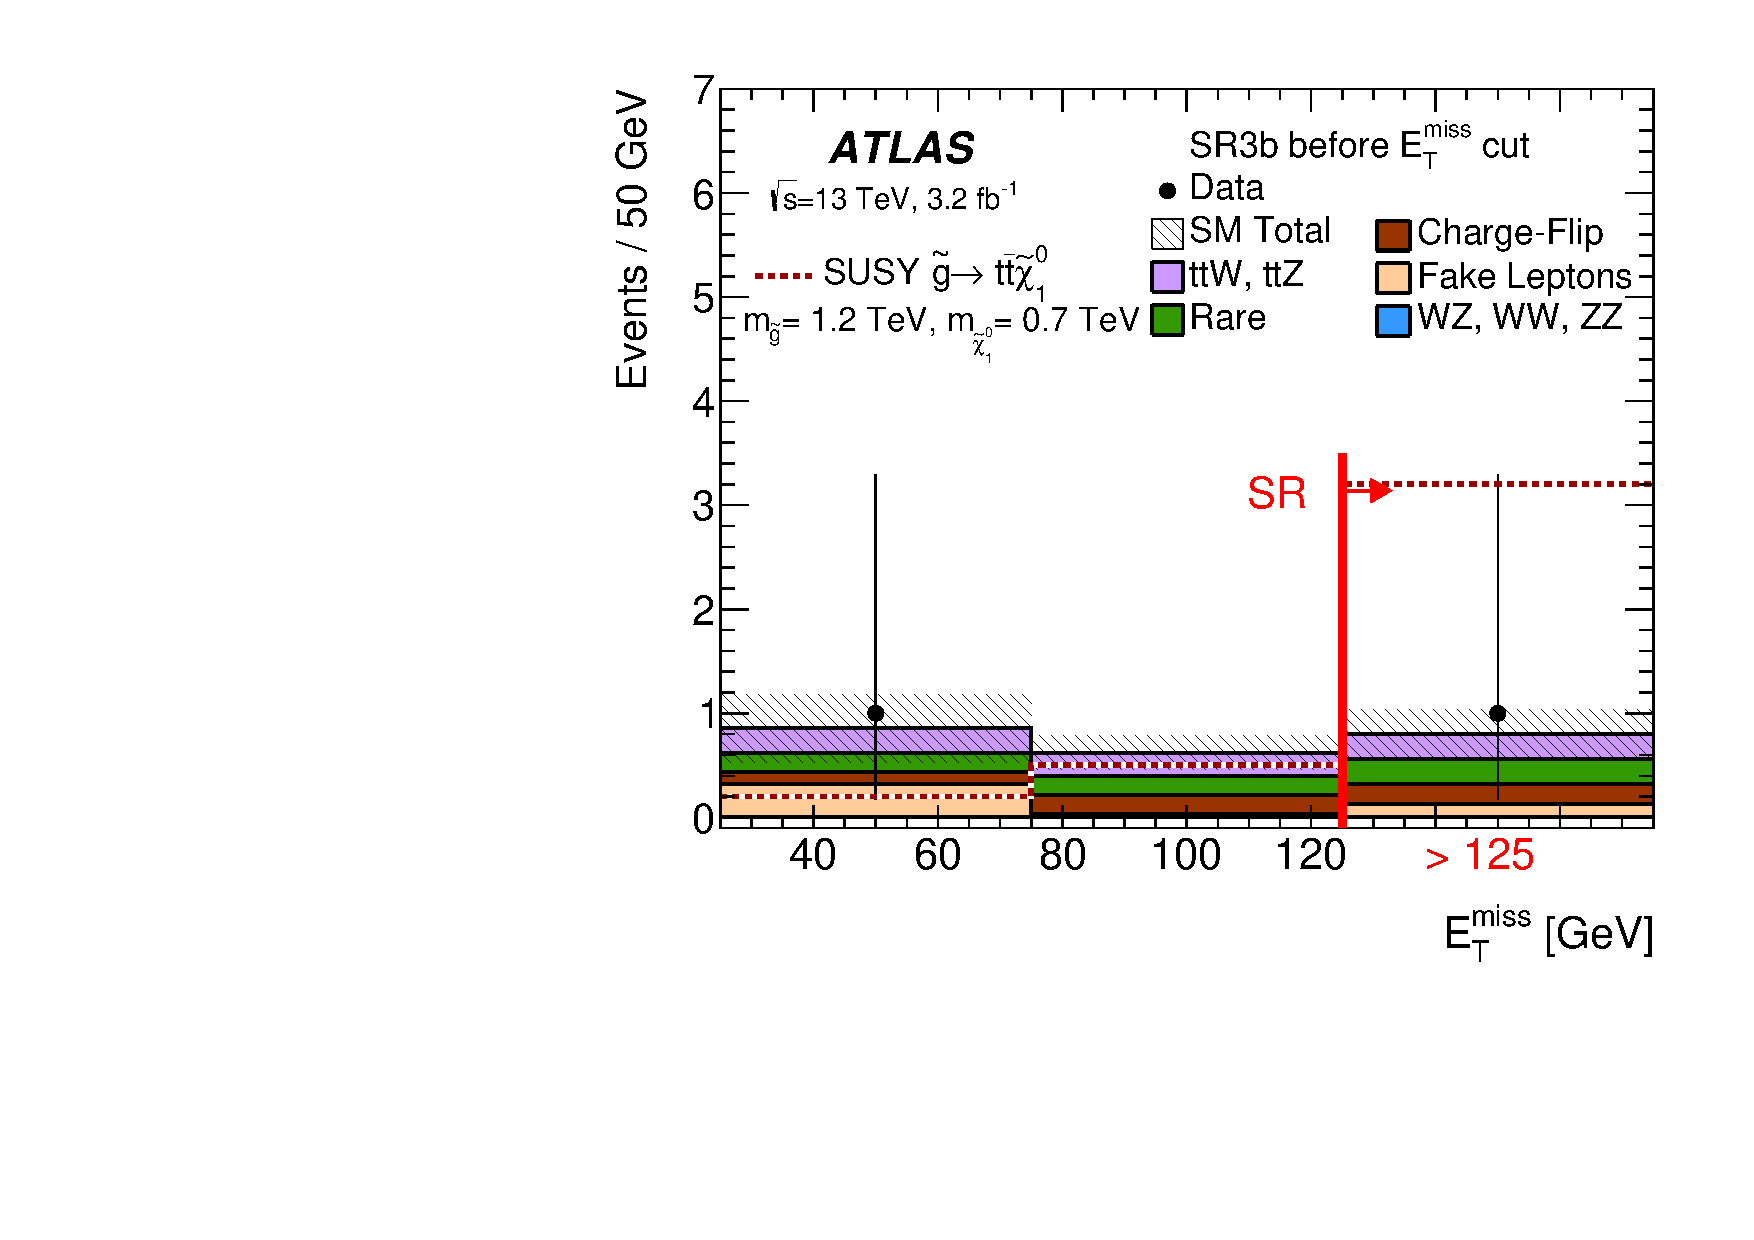
\includegraphics[width=\textwidth]{FIGURES/CONF_SR3b.pdf}
\caption{}\label{fig:Results_SR3b}\end{subfigure}
\caption{Missing transverse momentum distributions after (a) SR0b3j, (b) SR0b5j, (c) SR1b and (d) SR3b selection, beside the \met requirement. 
The results in the signal regions are shown in the last (inclusive) bin of each plot. 
The statistical uncertainties in the background prediction are included in the uncertainty band, 
as well as the theory uncertainties for the backgrounds with prompt SS/3L, 
and the full systematic uncertainties for data-driven backgrounds. 
The ``Fake leptons'' category corresponds to FNP leptons (see text), 
and the ``Rare'' category contains the contributions from associated production of $\ttbar$ with $h/WW/t/\ttbar$, 
as well as $tZ$, $Wh$, $Zh$, and triboson production. 
}
\label{fig:Results_SR_metD} 
\end{figure} 


Figure~\ref{fig:Results_SR_metD} shows the data \met distributions after the signal region selections (beside that on \met) in data 
together with the expected contributions from all the SM backgrounds with their total statistical and systematic uncertainties. 
For illustration, a typical SUSY signal distribution corresponding to the most relevant benchmark scenario 
in each SR is displayed.
The detailed yields for data and the different sources of SM background in the signal regions 
are presented in Table~\ref{tab:SR_yields}. 
The uncertainties amount to 22--34\% of the total background depending on the signal region. 
In all four SRs the number of data events exceeds the expectation but is consistent within the uncertainties, 
the smallest $p$-value for the SM-only hypothesis being 0.04 for SR0b5j. 
Out of the 14 events in the SRs, 2 of the events in SR1b and the 3 events in SR0b3j contain three leptons. 
None of those events contain three leptons of equal charge. 

In the absence of any significant deviations from the SM predictions, upper limits on possible BSM contributions to the signal regions are computed, 
in particular in the context of the SUSY benchmark scenarios described in Section~\ref{sec:intro}. 
The HistFitter framework~\cite{Baak:2014wma}, which utilises a profile-likelihood-ratio test~\cite{Cowan:2010js}, 
is used to establish 95\% confidence intervals using the CL$_\mathrm{s}$ prescription~\cite{Read_CLs}. 
The likelihood is built as the product of a Poisson probability density function describing the observed number of events in the signal region 
and Gaussian distributions constraining the nuisance parameters 
associated with the systematic uncertainties whose widths correspond to the sizes of these uncertainties; 
Poisson distributions are used instead for MC statistical uncertainties. 
Correlations of a given nuisance parameter across the different sources of backgrounds and the signal are taken into account when relevant. 
The statistical tests are performed independently for each of the signal regions. 

Table~\ref{tab:upperlimits} presents 95\% confidence level (CL) model-independent upper limits 
on the number of BSM events, $N_\mathrm{BSM}$, that may contribute to the signal regions. 
Normalising these by the integrated luminosity $L$ of the data sample, they can be interpreted as upper limits on the visible BSM cross-section $\sigma_{\rm{vis}}$, 
defined as the product $\sigma_{\rm{prod}}\times A \times\epsilon=N_\mathrm{BSM}/L$ of production cross-section, acceptance and reconstruction efficiency. 

\begin{table}[htb!]
\centering
\caption{Signal model-independent upper limits on the number of BSM events ($N_{\rm{BSM}}$) 
  and the visible signal cross-section ($\sigma_{\rm{vis}}$) in the four SRs. 
  The numbers (in parentheses) give the observed (expected under the SM hypothesis) 95\% CL upper
  limits. Calculations are performed with pseudo-experiments.
  The $\pm$1$\sigma$ variations on the expected limit due to the statistical and systematic uncertainties in the background prediction are also shown. 
}
\label{tab:upperlimits}
{\small
\renewcommand{\arraystretch}{1.4}
\begin{tabular*}{\textwidth}{@{\extracolsep{\fill}}lrrrr}
\noalign{\smallskip}\hline\hline\noalign{\smallskip}
         & SR0b3j         & SR0b5j     & SR1b & SR3b     \\[-0.05cm]
\noalign{\smallskip}\hline\hline\noalign{\smallskip}
$N_{\rm{BSM}}^{\rm{obs}}$ ($N_{\rm{BSM}}^{\rm{exp}}$) 
 & $5.9$  $({4.1}^{+1.6}_{-0.8})$
 & $6.4$ $({3.6}^{+1.2}_{-1.1})$
 & $8.8$ $({6.0}^{+2.6}_{-1.6})$ 
 & $3.8$ $({3.7}^{+1.1}_{-0.5})$ \\
$\sigma_{\rm{vis}}^{\rm{obs}}$ [fb] & 1.8 & 2.0 & 2.8 & 1.2\\
\noalign{\smallskip}\hline\hline\noalign{\smallskip}
  \end{tabular*}
}
\end{table} 

\begin{figure}[htb!]
\centering
\begin{subfigure}[t]{0.49\textwidth}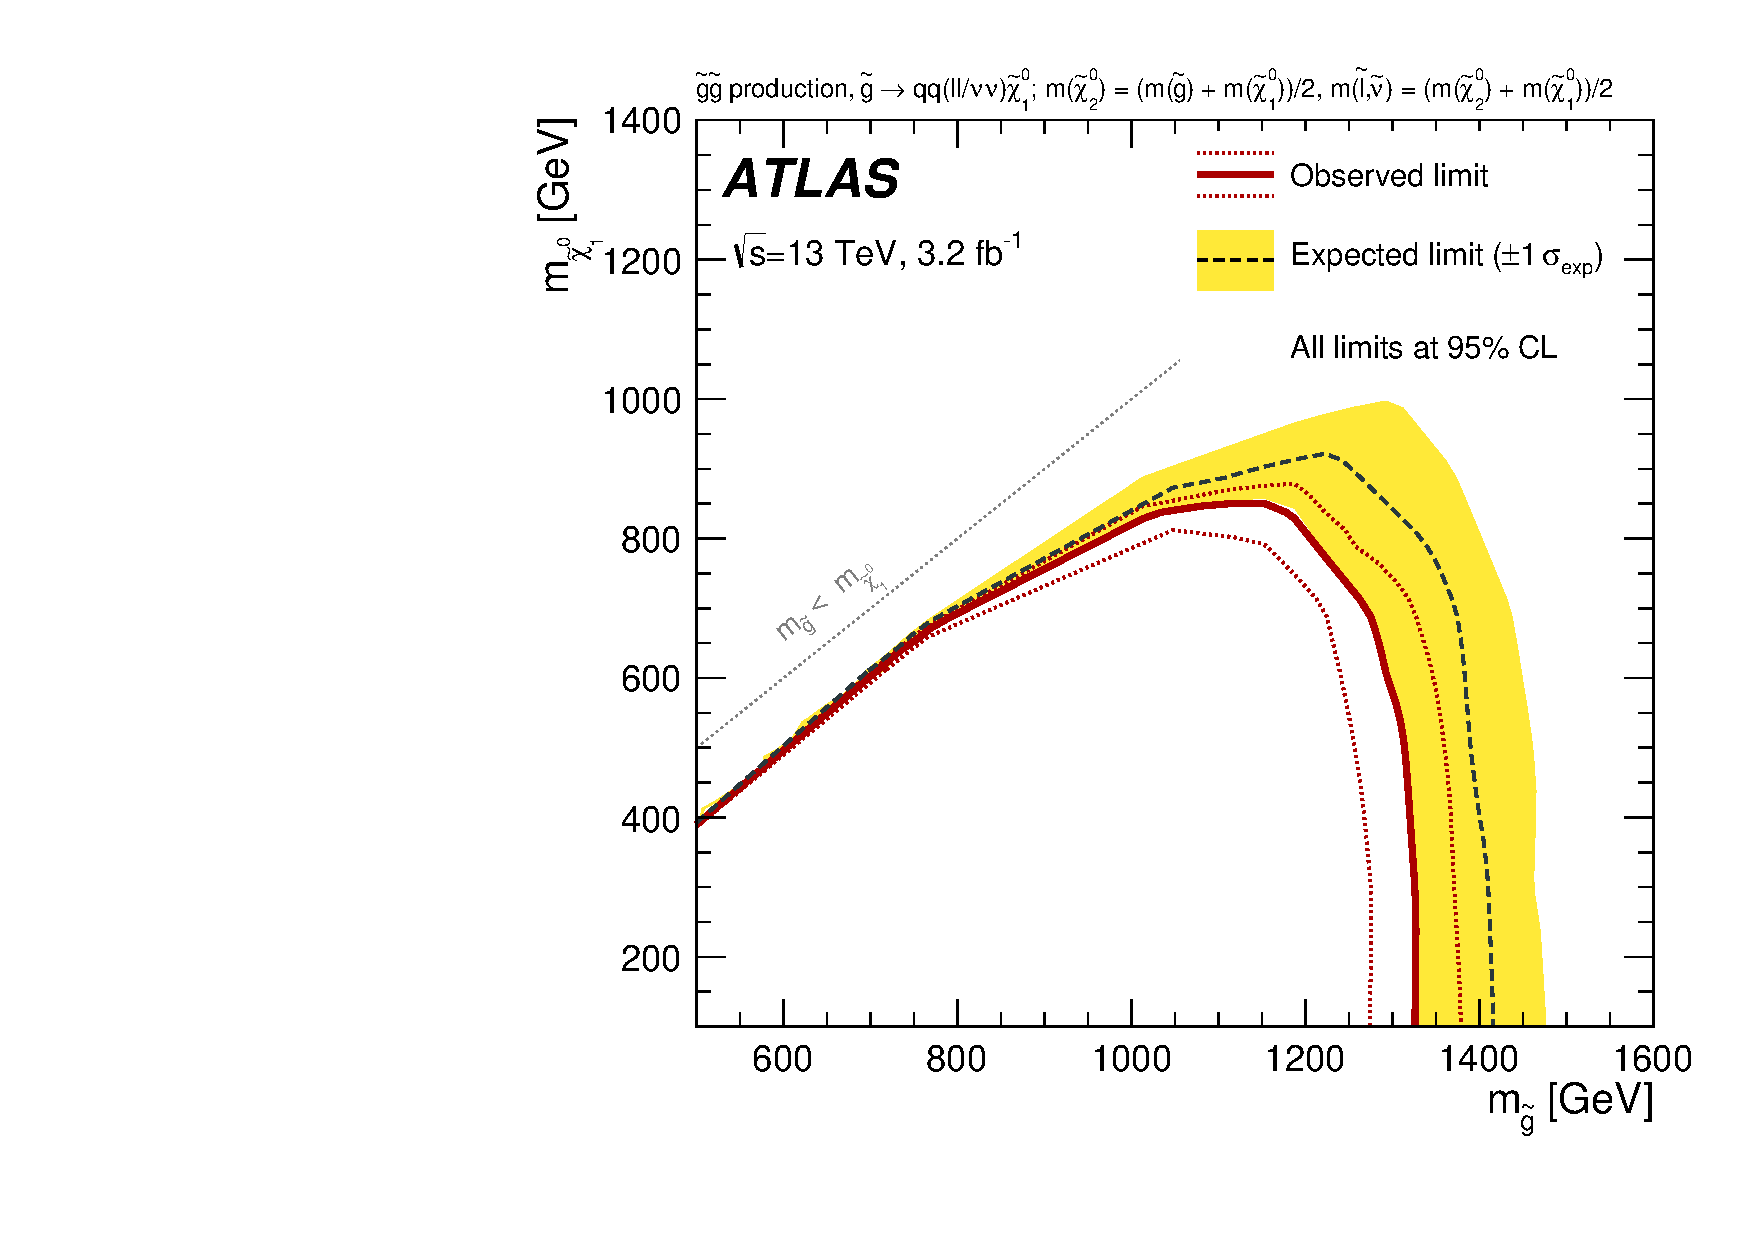
\includegraphics[width=\textwidth]{exclusion2015SameSign_SR0b3j.pdf}
\caption{$\gluino\to q\bar q \ell\ell\ninoone$ scenario, SR0b3j}\label{fig:limits_SR0b3j}\end{subfigure}
\begin{subfigure}[t]{0.49\textwidth}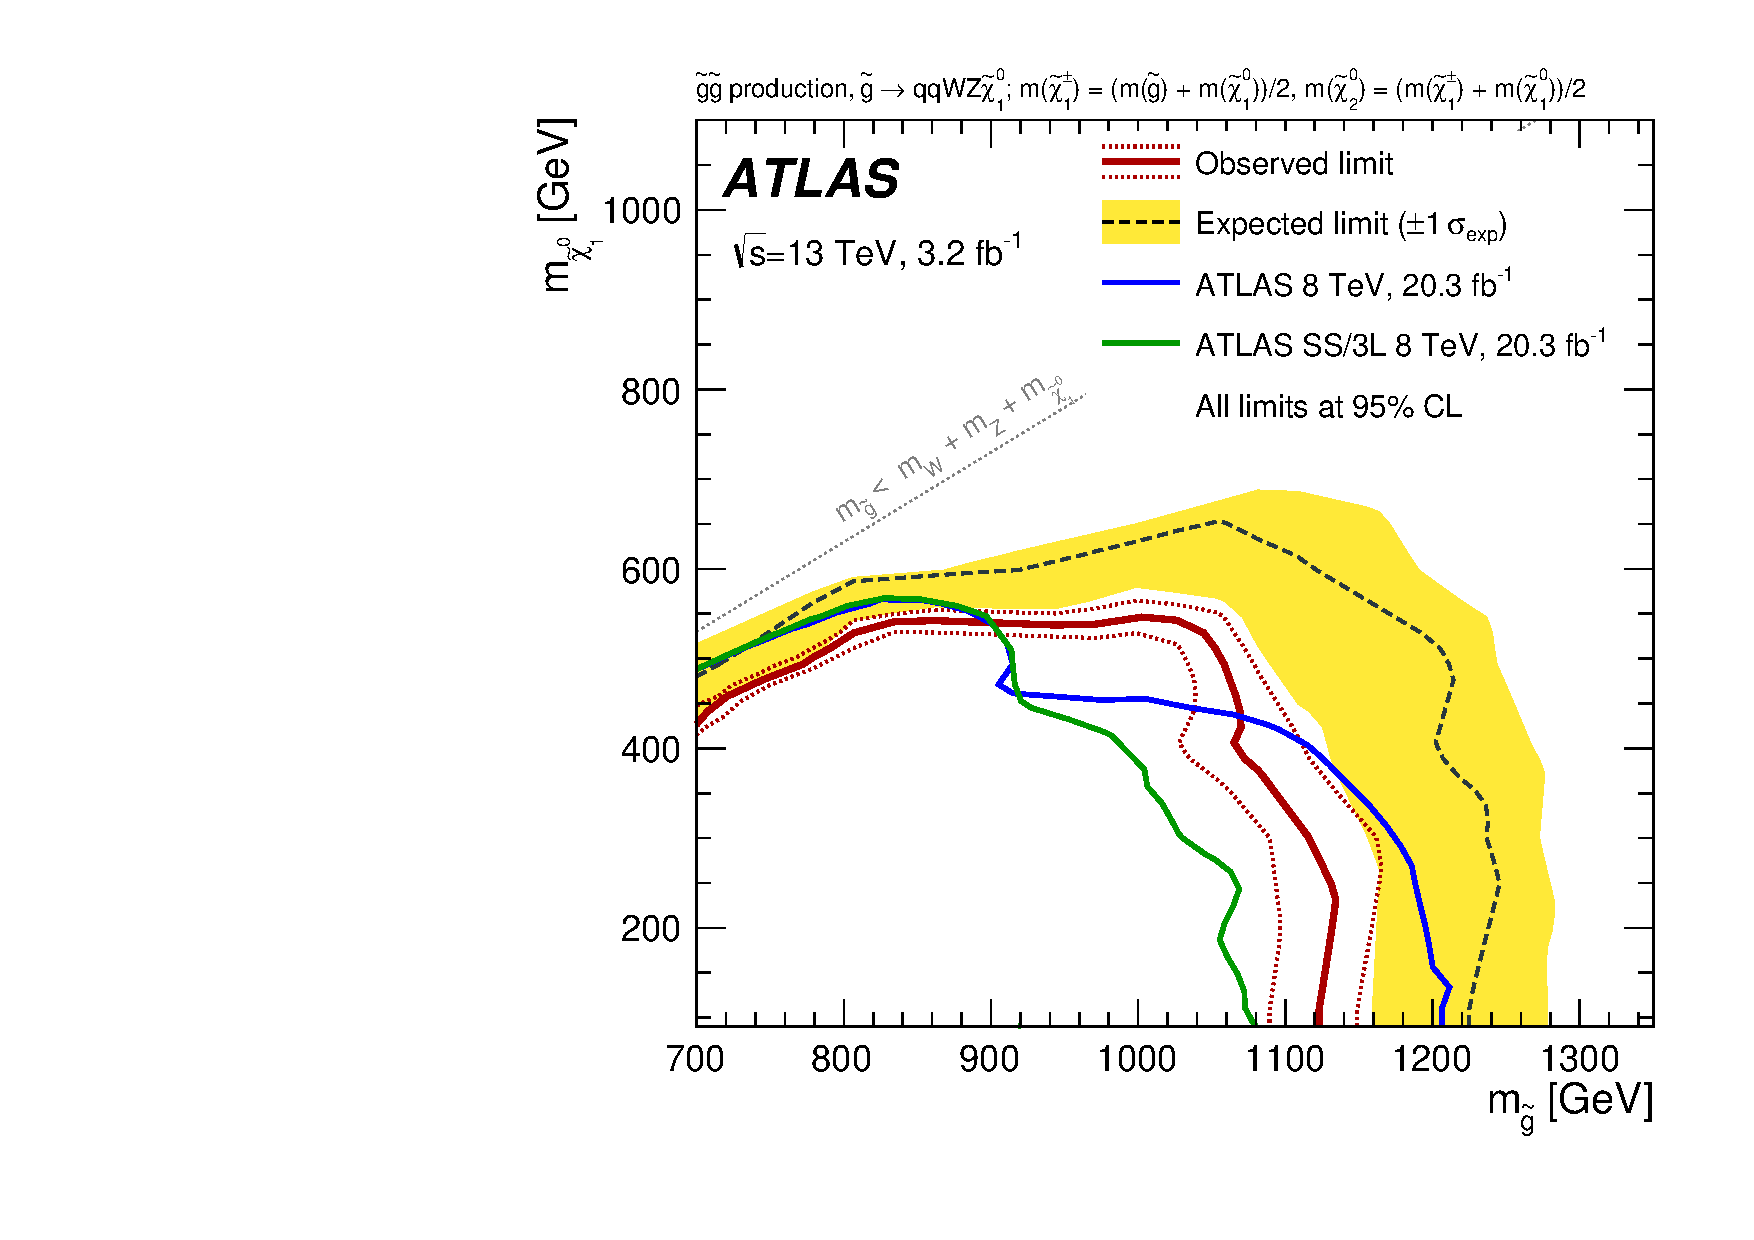
\includegraphics[width=\textwidth]{exclusion2015SameSign_SR0b5j.pdf}
\caption{$\gluino\to q\bar q' WZ\ninoone$ scenario, SR0b5j}\label{fig:limits_SR0b5j}\end{subfigure}
\par\bigskip
\begin{subfigure}[t]{0.49\textwidth}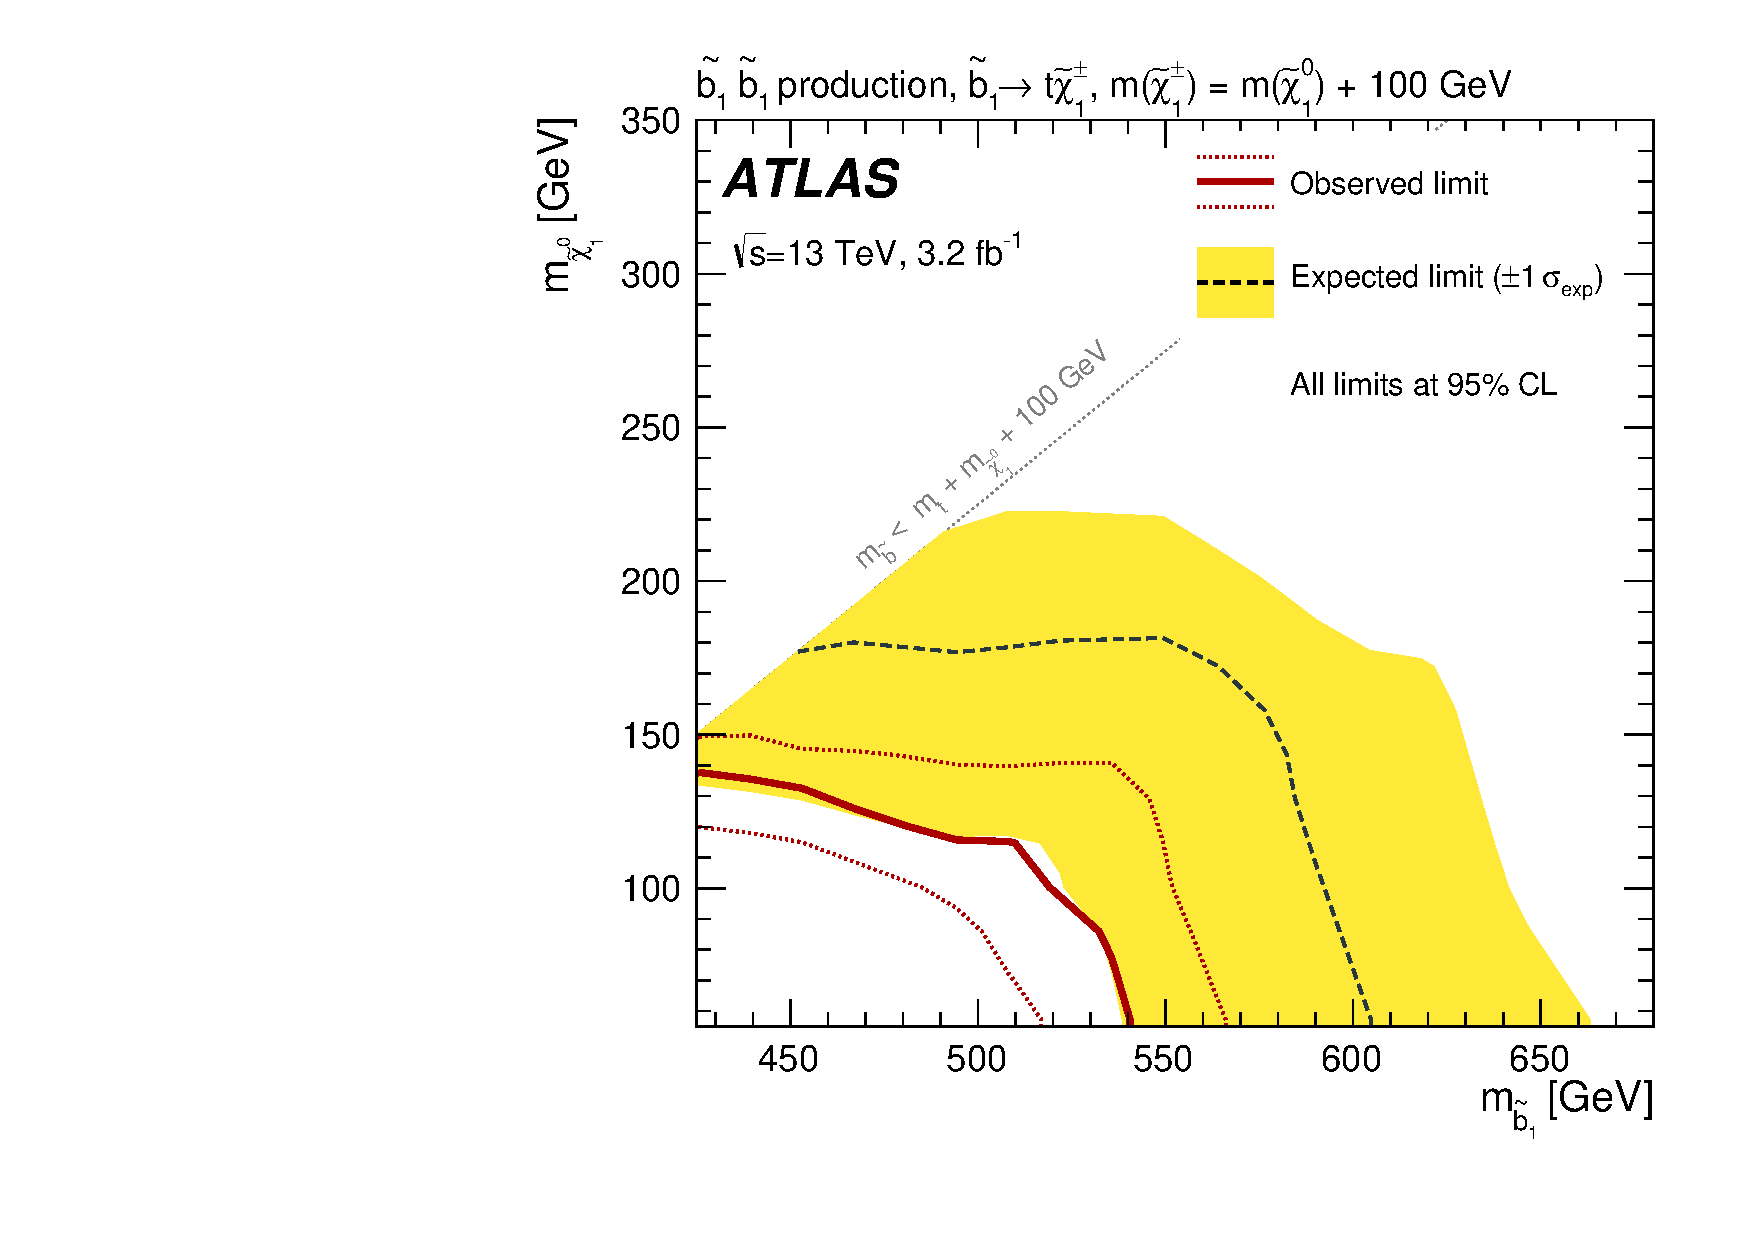
\includegraphics[width=\textwidth]{exclusion2015SameSign_SR1b.pdf}
\caption{$\sbottomone\to tW^-\ninoone$ scenario, SR1b}\label{fig:limits_SR1b}\end{subfigure}
\begin{subfigure}[t]{0.49\textwidth}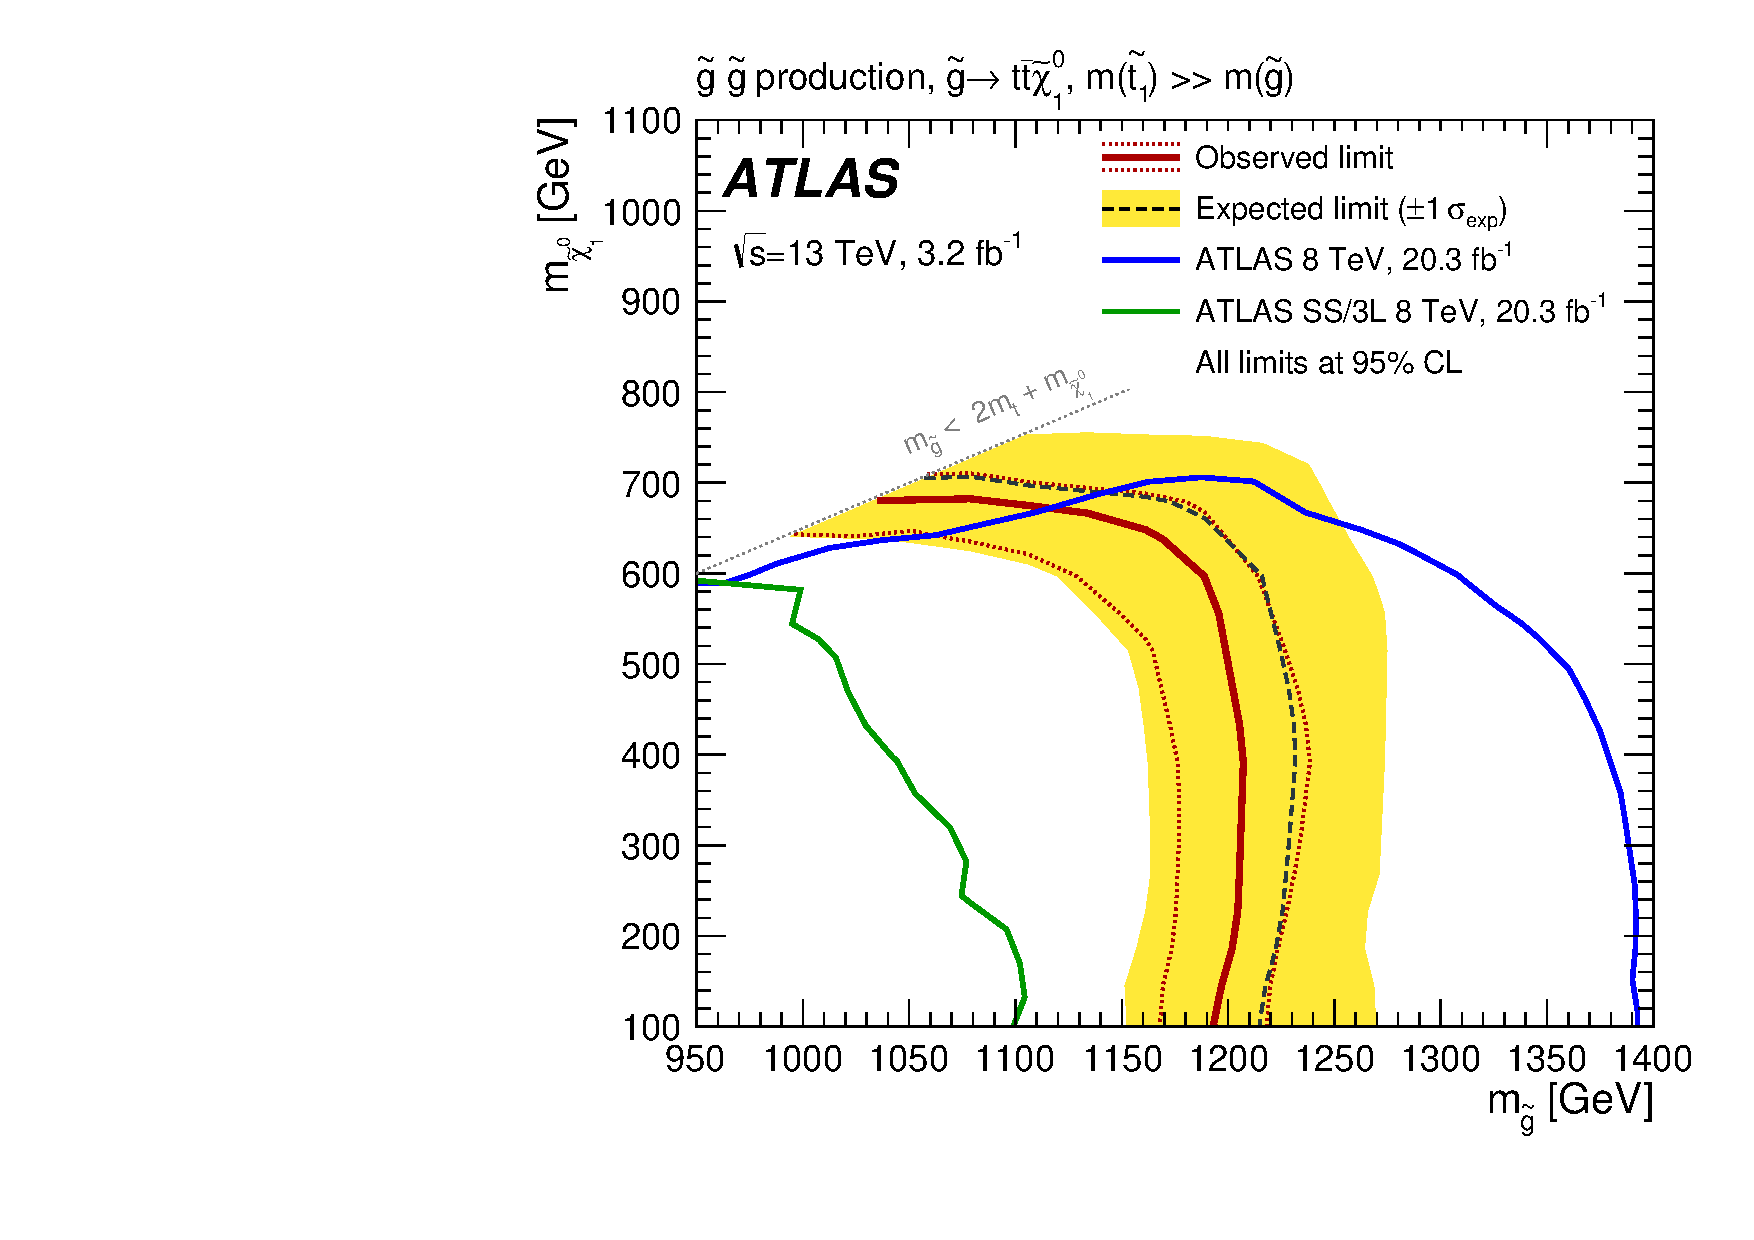
\includegraphics[width=\textwidth]{exclusion2015SameSign_SR3b.pdf}
\caption{$\gluino\to t\bar t\ninoone$ scenario, SR3b}\label{fig:limits_SR3b}\end{subfigure}
\caption{
Observed and expected exclusion limits on the \gluino, \sbottomone and \ninoone masses 
in the context of SUSY scenarios with simplified mass spectra 
featuring $\gluino\gluino$ or $\sbottomone\sbottomonebar$ pair production with exclusive decay modes. 
The signal region used to obtain the limits is specified for each scenario. 
The contours of the band around the expected limit are the $\pm$1$\sigma$ results, 
  including all uncertainties except theoretical uncertainties on the signal cross-section. The dotted lines around the observed
    limit illustrate the change in the observed limit as the nominal signal cross-section is scaled up and down
    by the theoretical uncertainty. All limits are computed at 95\% CL. 
    The diagonal lines indicate the kinematic limit for the decays in each specified scenario.  
For figures (b) and (d), results are compared with the observed limits obtained by previous ATLAS searches~\cite{paperSS3L,Aad:2015iea,Aad:2015pfx}. 
For figures (a) and (c), a direct comparison with earlier searches is not possible, due to differing model assumptions. 
}
\label{fig:Results_Limits} 
\end{figure} 

Exclusion limits are also set on the masses of the superpartners involved in the four SUSY benchmark scenarios considered in this analysis. 
Simplified models corresponding to a single production mode and with 100\% branching ratio to a specific decay chain are used, 
with the masses of the SUSY particles not involved in the process set to very high values. 
Figure~\ref{fig:Results_Limits} shows the limits 
on the mass of the $\ninoone$ as a function of the $\gluino$ or $\sbottomone$ mass. 
%For these results, asymptotic formulas~\cite{Cowan:2010js} are used to model the probability distribution of the test statistic. 
In some cases, the new limits set by this analysis can be compared 
with the existing limits set by the combination of ATLAS SUSY searches with 8 TeV data~\cite{Aad:2015iea,Aad:2015pfx}. 
For parts of the parameter space, the sensitivity reached with the 13 TeV dataset exceeds that of the 8 TeV dataset,
and additional parameter space regions can be excluded, especially for large neutralino masses. 

Signal models featuring gluino pair production with a subsequent gluino decay via $\ninotwo$ and light sleptons\\ 
($\gluino\to q\bar q\ninotwo\to q\bar q (\ell\slepton^*/\nu\tilde{\nu}^*)\to q\bar q(\ell^+\ell^-/\nu\nu)\ninoone$) 
are probed using SR0b3j (Fig.~\ref{fig:limits_SR0b3j}).
In this simplified model, the gluinos decay into $u\bar u$, $d\bar d$, $s\bar s$ or $c\bar c$ with equal probabilities, 
and the six types of leptons are also produced in the $\tilde\chi_2^0$ decays with equal probabilities. 
The $\ninotwo$ mass is set to $m_{\ninotwo}=(m_{\gluino} + m_{\ninoone})/2$, 
with the $\slepton$ and $\tilde{\nu}$ masses set to $m_{\slepton,\tilde{\nu}}=(m_{\ninotwo} + m_{\ninoone})/2$.
Gluino masses up to $m_{\gluino}\approx\SI{1.3}{TeV}$ for a light \ninoone and \ninoone masses up to $m_{\ninoone}\approx\SI{850}{GeV}$ for gluinos with $m_{\gluino}\approx\SI{1.1}{TeV}$ are excluded in this scenario. 

Similarly, models with gluino production  with a subsequent two-step gluino decay via $\chinoonepm$ and $\ninotwo$\\ 
($\gluino\to q\bar q \chinoonepm \to q\bar q W\ninotwo \to  q\bar q W Z \ninoone$) 
are probed with SR0b5j (Fig.~\ref{fig:limits_SR0b5j}).
In this simplified model, the gluinos decay into $u\bar u$, $d\bar d$, $s\bar s$ or $c\bar c$ with equal probabilities. 
The $\chinoonepm$ mass is set to $m_{\chinoonepm}=(m_{\gluino} + m_{\ninoone})/2$ and
the $\ninotwo$ mass is set to $m_{\ninotwo}=(m_{\chinoonepm} + m_{\ninoone})/2$; 
$W$ and $Z$ bosons produced in the decay chain are not necessarily on-shell. 
The exclusion limits in this scenario reach $m_{\gluino}\approx\SI{1.1}{TeV}$ (for light $\ninoone$) and $m_{\ninoone}\approx\SI{550}{GeV}$ (for $m_{\gluino}\approx\SI{1.0}{TeV}$).

Exclusion limits in a simplified model of bottom squark production with chargino-mediated $\sbottomone\to tW^-\ninoone$ decays are 
obtained with SR1b (Fig.~\ref{fig:limits_SR1b}).
In this model the $\chinoonepm$ mass is set to $m_{\chinoonepm}=m_{\ninoone} + \SI{100}{GeV}$.
The limits can reach mass values of $m_{\sbottomone}\approx\SI{540}{GeV}$ for a light $\ninoone$, 
while $m_{\ninoone}\lesssim\SI{140}{GeV}$ are also excluded for $m_{\sbottomone}\approx\SI{425}{GeV}$, 
significantly extending the previous limits obtained at $\sqrt{s}=8$~TeV~\cite{Aad:2015pfx} 
which excluded $m_{\sbottomone}\lesssim\SI{470}{GeV}$ for $m_{\ninoone}\approx\SI{60}{GeV}$ for a similar model.

Finally, SR3b is used to set limits on masses in a simplified model with 
gluino pair production and $\gluino\to t\bar t\ninoone$ decays 
via an off-shell top squark (Fig.~\ref{fig:limits_SR3b}). 
In that case, gluino masses of $m_{\gluino}\lesssim\SI{1.2}{TeV}$ are excluded for $m_{\ninoone}\lesssim\SI{600}{GeV}$, 
and $\ninoone$ masses up to $m_{\ninoone}\approx\SI{680}{GeV}$ are also excluded for $m_{\gluino}\approx\SI{1.05}{TeV}$. 



%\bibliography{sample_references}

% \backmatter




\end{document}


